\documentclass{article}

\usepackage[utf8]{inputenc}
\usepackage{hyperref}
\usepackage{xcolor}
\usepackage{graphicx}
\usepackage{graphicx}
\usepackage{tikzsymbols}
\usepackage{diffcoeff}
\usepackage{listings}
\usepackage{geometry}
\geometry{
  letterpaper,
  lmargin=1.5cm,
  rmargin=1.5cm,
  tmargin=2cm,
  bmargin=2cm,
  footskip=30pt,
  headheight=13.6pt}
\usepackage{amsthm}
\newtheorem*{remark}{Remark}
\newtheorem*{problem}{Problem}
\newtheorem*{definition}{Definition}
\usepackage{tikz}
\usepackage{pgfplots}
\usepackage{cancel}
\usepackage{neuralnetwork}
\usepackage{hyperref}

\usepackage{color}

\definecolor{dkgreen}{rgb}{0,0.6,0}
\definecolor{gray}{rgb}{0.5,0.5,0.5}
\definecolor{mauve}{rgb}{0.58,0,0.82}

\lstset{frame=tb,
  language=Python,
  aboveskip=3mm,
  belowskip=3mm,
  showstringspaces=false,
  columns=flexible,
  basicstyle={\small\ttfamily},
  numbers=none,
  numberstyle=\tiny\color{gray},
  keywordstyle=\color{blue},
  commentstyle=\color{dkgreen},
  stringstyle=\color{mauve},
  breaklines=true,
  breakatwhitespace=true,
  tabsize=3
}

\title{Introduction to Deep Learning}
\author{Jai Sharma}
\date{\today}
\begin{document}

\maketitle
\clearpage
\hspace{100mm}
\clearpage
\tableofcontents
\clearpage
\part{Foreword}
\section*{To the Reader}
Deep Learning is one of the greatest areas of research and practical applications today; it is a gold mine waiting to be tapped into. I am really proud of you for taking your first step to learning about this great subject by reading this text. 
\\
\\
In this text, we will start by exploring the applications of Deep Learning and why it has become so widespread in its use. We will then examine some elementary Machine Learning algorithms such as Linear Regression and Logistic Regression, both of which will give us a nice foundation to learn about Neural Networks. Next, we will explore Neural Networks at a high level without going too much into the mathematical side.
\\
\\
After this high level approach, we delve into the basic mathematical understanding needed for Deep Learning, including Linear Algebra and Calculus. We develop the tools we will need to derive the parameter updates for Linear Regression, Logistic Regression, and Neural Networks. These derivations are a essential to explaining how Machine Learning and Deep Learning algorithms ``learn'' from patterns.
\\
\\
The second part of the text focuses on implementing the skills in the first part in code. We will be using Python here because of its famous libraries such as NumPy and Matplotlib. We will conclude the text with implementations of Linear Regression, Logistic Regression, and Neural Networks from scratch in Python.
\\
\\
I hope this book will not only provide instruction on the concepts behind Deep Learning, but also the interest to explore its riches. Thank you for reading this text.
\clearpage

\part{Introduction}
\clearpage
\section{What is Deep Learning?}
As our world becomes more digitized, more and more information is being structurally recorded. As a result, a plethora of enormous data sets have been made, many of these being available to the common public. \color{blue}\href{https://www.kaggle.com/}{Kaggle}\color{black}, a child company of Google, has become one of the most popular hubs for accessing such data sets. 
\\
\\
As such, it has become increasingly important for large industries and companies to be able to effectively understand and use this gathered information. This necessity has inspired the development of the realm of data analysis. 
\\
\\
Machine Learning is one of the sub-branches of data analysis in which humans employ computers to identify and extrapolate patterns in data. 
\\
\\
Deep Learning is the use of Machine Learning through a method known as ``Neural Networks.'' Neural Networks are a mechanism which tries to mimic the human brain in terms of how patterns in data are identified. 

\paragraph{Purpose}The goal of this handout is to discuss the technicalities and specifics of Deep Learning models so that you may fully understand the fundamentals of Deep Learning as well as how to make a Deep Learning model yourself.

\section{Applications of Deep Learning}
You likely experience the impacts of Machine Learning many times on a daily basis. Many practitioners have begun to use Neural Networks as opposed to other models in Machine Learning, which means that you are also likely deeply affected by Deep Learning in your daily routines. 
\\
\\
Here are some common examples of Machine Learning and Deep Learning at work:
\begin{itemize}
    \item Weather prediction;
    \item Content recommendation systems (Netflix, YouTube, Amazon, Spotify, etc.);
    \item Spam filters for email;
    \item Supply and demand forecasting in business; 
    \item Autonomous driving vehicles;
    \item Photo recognition systems;
    \item Speech recognition systems;
    \item Smart devices (Siri, Cortana, Google Home, Amazon Echo, etc.);
    \item Search Engines (Google, etc.);
    \item Translation Systems (Google Translate, etc.);
    \item Spellcheck (Google Docs, Grammarly, etc.);
    \item Medical research and imaging;
    \item Biometric scans (fingerprint, facial recognition, etc.);
    \item Deep fakes.
\end{itemize}
The list goes on, and on, and on\ldots
\\
\\
Hopefully, you were able to relate at least one of these items to your personal life. If so, you know the value of Machine Learning from a practical perspective. 
\\
\\
What's more is that the hype has only just begun! While shown to be colossal in its implications, Machine Learning is a relatively young topic, and a multitude of research is being done for it. 
\\
\\
If you do not have any project ideas, look for data sets on Kaggle that interest you! Remember, anywhere that there is data, there is a chance for Machine Learning to be applied. Kaggle also has many \color{blue}\href{https://www.kaggle.com/competitions}{competitions }\color{black} on their website which you can take inspiration from (or enter). 

\section{Deep Learning v.s. Other Machine Learning Algorithms}
There are tons of models out there. Here are some:
\begin{itemize}
    \item Linear/Polynomial Regression;
    \item Logistic Regression;
    \item Support Vector Machines;
    \item K Means Clustering.
\end{itemize}
Out of all of these, why do we choose to use Neural Networks?
\\
\\
To answer this question, we examine why other models were even made in the first place. Consider the following image (\color{blue}\href{https://lilianweng.github.io/lil-log/2017/06/21/an-overview-of-deep-learning.html}{source link}\color{black}):
\[\includegraphics[scale = 0.5]{data_size_vs_model_performance.png}\]
Consider the left side of the vertical dashed purple line. This is represents the size of the data sets prior to digitization of information. At this time, data sets were small, and using any kind of model seemed satisfactory.
\\
\\
However, as digitization began, data sets became more like the ones to the right of the line. They were bigger, and at this time, the performance of Neural Networks and Deep Learning shined through. 
\\
\\
Compared to Deep Learning, other models are just not as outstanding anymore, which is why many systems are making a switch. 

\section{Linear Regression}
Say you wished to forecast daily temperature. There are an infinite number of values which can be the temperature.
\\
\\
When the entity we wish to predict or extrapolate can take on a whole range of values, as in this example, we say that we have a \textbf{regression} problem.
\\
\\
One introductory form of regression is Linear Regression. In this section, we will explore Linear Regression, which is a core part of Machine Learning.

\subsection{Computing the Hypothesis}
Continuing with our temperature forecasting example, say we wish to predict the temperature on a given day in a particular place in the world using the month of the year. 
\\
\\
We will label the months as January-1, February-2, March-3, etc. Then, let $h(x)$ be a function that computes the hypothesis, or prediction, of the temperature given the month number $x$.
\\
\\
Let's say we know that $h(x)=-x+70$ (we will discuss how to find $h(x)$ later). Then, we can calculate the (approximate) temperature on a given day.
\\
\\
Maybe I want to plan a party on April 1st and want to know what the weather will be like. April corresponds to 4, as it is the fourth month of the year. Then, our hypothesis becomes: $h(x)=h(4)=-4+70=66$ degrees. Similarly, I can find the (approximate) temperature on any given day if I know the month the day is in. 
\\
\\
Unfortunately, I decide that knowing the month is not enough. I want to \textbf{give my model more information so that it can make a more educated prediction.}
\\
\\
Let us adjust our function $h(x)$ to take in two inputs: the month ($x_1$) as well as the year of the given day we wish to predict ($x_2$). 
\\
\\
Then, let's say we know that our adjusted function is $h(x_1,x_2)=-2x_1+0.001x_2+70$. Then, we can calculate the temperature of a given day using the month and year that the day is in. 
\\
\\
Let's use our example of April 1st again. This time we must also know the year on which the party will occur. Let the party occur on April 1st, 2020. Then, $x_1=4$ and $x_2=2020$. Make sure you see why. Then, the temperature hypothesis is \[h(x_1,x_2)=h(4,2020)=-2(4)+0.001(2020)+70=-8+2.02+70=64.02\text{ degrees}.\]
This is how we compute the Linear Regression hypothesis. Let us generalize this.
\\
\\
Say we are doing a regression problem in which we wish to predict or hypothesize some entity (temperature of a given day in the last case) given some inputs $x_1,x_2,x_3,x_4,\ldots$ These inputs are called \textbf{features} (or $x$-values) and what we wish to predict is called the \textbf{label} (or $y$-values). 
\\
\\
Then, the objective of Machine Learning is to find a function that maps our features to our labels. This function is called the \textbf{hypothesis function}, as mentioned earlier.
\\
\\
When given a data set, we often wish to evaluate our model by using the given inputs to generate a \textbf{hypothesis} using our hypothesis function and comparing this prediction to the actual label of the entry in the data set. Our prediction is sometimes called the \textbf{predicted value} and the actual $y$-value recorded in the data set is called the \textbf{observed value}. 
\\
\\
Linear regression is a means to an end to find a hypothesis function to map the input features to the output labels. In general, linear regression hypothesis functions look like the following:
\[h(x_1,x_2,\cdots,x_n,\theta_0,\theta_1,\theta_2,\cdots,\theta_n)=\theta_0+\theta_1x_1+\theta_3x_3+\theta_4x_4+\ldots+\theta_nx_n,\]
where $x_1,x_2,\cdots,x_n$ are the input features, $h$ is the hypothesis function, and $\theta_0,\theta_1,\cdots,\theta_n$ are the \textbf{parameters} or \textbf{weights}. 
\\
\\
In the previous example, $h(x_1,x_2)=-2x_1+0.001x_2+70$. Here, -2, 0.01, and 70 were the parameters, or weights. Notice that $\theta_0=70$ in this example. The parameter $\theta_0$ is always added in the hypothesis regardless of the value of any input. $\theta_0$ is sometimes called the \textbf{bias term}. The output of the function $h$ is sometimes called $\hat{y}$ for shorthand.
\\
\\
Notice that if there were only one input $x_1$, then the hypothesis would be $h(x_1)=\theta_0+\theta_1x_1$. Taking $\theta_0$ and $\theta_1$ to be constants $b$ and $m$, respectively, we get $\hat{y}=h(x_1)=b+mx_1$ or 
\[\hat{y}=mx_1+b.\]
You may remember from your Algebra knowledge that this is just the equation of a line in 2 dimensions! In fact, a linear regression hypothesis which takes $n$ features inputs is actually the equation of a line in $n+1$ dimensions! Hence, the name ``Linear'' Regression.
\\
\\
\begin{remark}[Another Perspective]
Qualitatively, this is what Linear Regression is doing: Linear Regression takes each of the inputs, multiplies each by some number, takes the sum, and adds a constant. And ta-da! A hypothesis!
\end{remark}

\subsection{Linear Regression Cost Function}
The goal of Linear Regression (and any other type of regression) is to learn the hypothesis function for a data set by learning the values of the parameters. 
\\
\\
We will go over how to do this, but first, we must talk about a way to evaluate the model. For Machine Learning problems, we use \textbf{cost functions} to evaluate our models. This cost function then becomes what we wish to optimize. 
\\
\\
In linear regression, we use the \textbf{Mean Squared Error} (MSE) as our cost function. 
\\
\\
For one example in our data set, this is how we would compute the cost function:
\begin{enumerate}
    \item Compute the hypothesis $\hat{y}$ for the given example;
    \item If the observed value for the example is $y$, then the cost for this example is $(\hat{y}-y)^2$
\end{enumerate}
Then, to evaluate the cost for the $m$ examples in our data set, we simply take the average of all of the costs and divide by 2. Namely, the cost function, typically denoted $J(x_1,x_2,\cdots,x_n,\theta_0,\theta_1,\theta_2,\cdots,\theta_n)$, is:
\[J(x_1,x_2,\cdots,x_n,\theta_0,\theta_1,\theta_2,\cdots,\theta_n)=\frac{1}{2m}\sum_{i=1} ^{m} (y_i-\hat{y}_i)^2,\]
where $y_i$ and $\hat{y}_i$ are the observed and predicted values for the $i$th example in the data set, respectively.
\begin{remark}
Don't get too warped up in this technical definition of the cost function. Just understand what the cost function is meant to be used for and how to calculate the cost for one example in the data set. 
\end{remark}
The cost function is often hard to visualize, but you can think of it as something like this: 
\[
\begin{tikzpicture}
\begin{axis}[
    axis lines = left,
    xlabel = $\theta_i$,
    ylabel = Cost,
    ticks = none,
    xmin = -12, ymin=-5,
]
\addplot [
    domain=-10:10, 
    samples=100, 
    color=black,
]
{x^2};
\addplot[mark=*] coordinates {(0,  0)};
\end{axis}
\end{tikzpicture}
\]
Essentially, as we vary the values of the parameters, we get different values for the cost function. Since the cost function measures the error of the predictions (Why?), we wish to minimize our cost. In this example, we wish to make $\theta_i$ coincide with the dot above, as it is the minimum. In a similar way, we would optimize all of our parameters. But how do we go about doing that?
\subsection{Parameter Update}
In this section, we see how to adjust our parameters to optimize the cost function. 
\\
\\
Consider the following image: 
\[
\begin{tikzpicture}
\begin{axis}[
    axis lines = left,
    xlabel = $\theta_i$,
    ylabel = Cost,
    ticks = none,
    xmin = -12, ymin=-5,
]
\addplot [
    domain=-10:10, 
    samples=100, 
    color=black,
]
{x^2};
\addplot[mark=*] coordinates {(0,  0)};
\addplot[mark=*] coordinates {(5,  25)};
\end{axis}
\end{tikzpicture}
\]
Say that our $\theta_i$ currently coincides with the point on the right above. Then, we wish to decrease our parameter value in order to get closer to the \textbf{global minimum}, or the lowest possible cost, which is in the center of the graph. But how would we know that we must decrease the value without graphing?
\\
\\
Consider the following line added to the graph:
\[
\begin{tikzpicture}
\begin{axis}[
    axis lines = left,
    xlabel = $\theta_i$,
    ylabel = Cost,
    ticks = none,
    xmin = -12, ymin=-5,
]
\addplot [
    domain=-10:10, 
    samples=100, 
    color=black,
]
{x^2};
\addplot [
    domain=2.5:10, 
    samples=100, 
    color=black,
]
{x*10-25};
\addplot[mark=*] coordinates {(0,  0)};
\addplot[mark=*] coordinates {(5,  25)};
\end{axis}
\end{tikzpicture}
\]
The \textbf{slope} of this line is positive because it is pointing in the right upward direction. 
\\
\\
Now, consider this alternate case:
\[
\begin{tikzpicture}
\begin{axis}[
    axis lines = left,
    xlabel = $\theta_i$,
    ylabel = Cost,
    ticks = none,
    xmin = -12, ymin=-5,
]
\addplot [
    domain=-10:10, 
    samples=100, 
    color=black,
]
{x^2};
\addplot [
    domain=-10:-2.5, 
    samples=100, 
    color=black,
]
{x*(-10)-25};
\addplot[mark=*] coordinates {(0,  0)};
\addplot[mark=*] coordinates {(-5,  25)};
\end{axis}
\end{tikzpicture}
\]
Now, the slope of the line is negative because it is pointing in the right downward direction. 
\\
\\
We call the lines that were just drawn \textbf{tangent lines} because in the general vicinity of the given points, they \textbf{only intersect the graph of the cost function at that point}. 
\\
\\
In the next parts, we will discuss exactly how to find the slopes of these lines for Machine Learning cost functions and functions in general. 
\\
\\
For now, we examine the presented cases:
\begin{enumerate}
    \item The value of $\theta_i$ is more than the optimal value. Then, as we saw, the slope of the tangent line is \textbf{positive} and we wish to \textbf{decrease} our parameter value. 
    \item The value of $\theta_i$ is less than the optimal value. Then, as we saw, the slope of the tangent line is \textbf{negative} and we wish to \textbf{increase} our parameter value.
\end{enumerate}
Because of these two cases, it makes sense if we were to adjust the value of $\theta_i$ through doing the following: 
\[\theta_i:=\theta_i-\alpha\diff{J}{\theta_i},\]
where the $:=$ means that we replace $\theta_i$ with the value on the right, $\alpha$ is a constant, and $\diff{J}{\theta_i}$ is the slope of the tangent line. 
\\
\\
Notice that no matter where $\theta_i$ is with respect to the optimal value of $\theta_i$, we always make the parameter update in the correct manner using this method.
\begin{remark}
Make sure you understand how this parameter update satisfies both of the above cases before you move on!
\end{remark}
\\
\\
This parameter update is not specific to Linear Regression. This is how parameters are updated for any type of Machine Learning model. 
\begin{remark}
If this is your first time reading this, then do not worry if you do not understand why we use the seemingly arbitrary ``slope of the tangent line." Focus more on convincing yourself that this method will update the parameters correctly. As you will see, we use the slope of the tangent line simply because it is easy to find its value.
\end{remark}
\begin{remark}[Alpha]
Alpha ($\alpha$) is a seemingly random constant that appears in the parameter update. Since it is defined to be positive, it does not affect the direction in which we adjust our parameters; rather, it controls the magnitude by which we make the adjustment. Too small of an $\alpha$ value and we make too small of a step in the direction to the optimal parameter value. Too large an $\alpha$ value and we make too large of a step in the direction to the optimal parameter value and we ``overshoot" the minimum. If we overshoot enough, our parameter value can \textbf{diverge}. Because of these effects, $\alpha$ is called the \textbf{learning rate} of a Machine Learning model. 
\end{remark}

\subsection{Gradient Descent}
Now, it is time to put our ideas together in a concrete fashion. In this section, we introduce the idea of \textbf{Gradient Descent} and explain how it is used in finding the parameters for a Machine Learning model. These learned parameters can then be used to create the hypothesis function, which is the goal of Machine Learning. 
\\
\\
Gradient Descent is described very generally and briefly by the following steps:
\begin{enumerate}
    \item \textbf{Initialize Parameters:} Parameters have to start somewhere! Sometimes, we initialize them to be 0, and other times at random. This depends on the parameter type and the model we are using.
    \item \textbf{Compute the Cost Function Using the Current Hypothesis Function:} We use our existing hypothesis function $h$ to compute our hypothesis $\hat{y}$. Then, we use $\hat{y}$ and the observed values $y$ to compute the cost function $J$. 
    \item \textbf{Parameter Update:} We compute the slope of the tangent line to the cost function and use this to update our parameters and make our hypothesis function just a bit better as talked about in the last section. Note that we can often update the parameters without ever computing the cost, but the cost is a helpful indicator that your model is working as intended.
    \item \textbf{Repeat!:} We repeat steps 2 and 3 over, and over, and over\ldots until our cost is low enough that we are happy with it. 
\end{enumerate}
This above process is the core of most all Machine Learning algorithms, so make sure you know it by heart!
\\
\\
For Linear Regression, we initialize all of our parameters to be 0. We know how to compute the cost, and we know about the parameter update except for the slope of the tangent line part. We will cover this specific detail later. For now, make sure you understand how Machine Learning algorithms are trained (at a high level).

\webfig{idl-linreg}


\section{Logistic Regression}
Logistic Regression is also one of the core parts of Neural Networks. Arguably, Neural Networks is just a series of Logistic Regression Functions. In this section, we discuss Logistic Regression as an extension of Linear Regression.

\subsection{Logistic Regression Hypothesis}
Once you understand what Linear Regression is doing, the Logistic Regression hypothesis function is quite simple to understand. 
\\
\\
Let our hypothesis $h(x_1,x_2,\cdots,x_n,\theta_0,\theta_1,\theta_2,\cdots,\theta_n)$ be defined as the following:
\[h(x_1,x_2,\cdots,x_n,\theta_0,\theta_1,\theta_2,\cdots,\theta_n)=\sigma(g(x_1,x_2,\cdots,x_n,\theta_0,\theta_1,\theta_2,\cdots,\theta_n)),\]
where $g(x_1,x_2,\cdots,x_n,\theta_0,\theta_1,\theta_2,\cdots,\theta_n)$ is a Linear Regression hypothesis function and 
\[\sigma(x)=\frac{1}{1+e^{-x}}\]
for any real number $x$. 
\\
\\
Here is the graph of $\sigma(x)$:
\[
\begin{tikzpicture}
\begin{axis}[
    axis lines = center,
    xlabel = $x$,
    ylabel = $\sigma(x)$,
    xmin = -10, xmax=10, ymin=-0.2, ymax=1.2
]
\addplot [
    domain=-10:10,
    samples=100, 
    color=black,
]
{1/(1+e^(-x))};
\end{axis}
\end{tikzpicture}
\]
What is the hypothesis function doing? It is taking the output of some Linear Regression function and feeding it into the sigmoid function $\sigma(x)$, a function which outputs a number between 0 and 1. 
\\
\\
0 and 1? That sounds like the range we use for \textit{probability}. In fact, that is exactly what it is! Essentially, the Logistic Regression hypothesis function maps its inputs to a \textbf{probability}. Now why would this be useful?
\subsection{Applications of Logistic Regression}
In Linear Regression, our output can take on a near infinite number of values. We call this a \textbf{continuous} output. Logistic Regression, however, is more useful when our output can only take on a finite number of values. We call this a \textbf{discrete} output. 
\\
\\
Here are some questions/problems that could be aided using Logistic Regression:
\begin{itemize}
    \item Will it rain tomorrow or not? Here, there are two options: 1) Yes, it will rain, and 2) No, it will not rain.
    \item Is a given email spam or not? This also has two options.
    \item Is a given product that was produced in a factory defective? Again, there are two alternatives. 
    \item Identify hand-written digit. This problem has ten options: $0,1,2,\cdots,9$
\end{itemize}
For the first three, we can train a Logistic Regression model to find the probability for each event happening. For the last one, however, we will need to train 10 different models. Namely, we will need to train one model to output the probability that the digit is 0, one model to output the probability that the digit is 1, and so on. To determine what digit a given digit is, we will trust the model with the highest probability.
\begin{remark}
For this last example, Neural Networks can output more than one probability, which means that we can train just one model instead of 10.
\end{remark}
\\
\\
After we find the probabilities, we can decide our final prediction. If $\hat{y}\geq 0.5$, we output ``1," meaning that we believe that it will rain, or the email is spam, or the given product is defective, following the previous examples. If $\hat{y}< 0.5$, we output ``0," meaning that we believe that it will \textit{not} rain, or the email is \textit{not} spam, or the given product is \textit{not} defective.
\\
\\
Now, how do we train our model? For that, we will need to define a cost function for Logistic Regression.
\begin{remark}
The name ``Logistic Regression" is somewhat misleading. Logistic Regression is actually a kind of \textbf{classification}, not regression. This is because we have a discrete output range instead of a continuous one. In general, classification refers to identifying and ``classifying" and example based on its input features. 
\end{remark}

\subsection{Logistic Regression Cost Function}
For Logistic Regression, we use the same algorithm as the one for Linear Regression: Gradient Descent. We initialize all our parameters to 0, but how do we measure the cost? Do we use MSE (which we used for Linear Regression) or something else?
\\
\\
It turns out that MSE is no longer a desirable cost function for Logistic Regression. In Linear Regression, we were measuring the ``distance" between our predictions and the observed values. We could do this because our output was continuous. However. It does not make sense to do the same thing anymore since the output will always be between 0 and 1. 
\\
\\
So, how do we measure the cost? If $y$ is the observed value (which is always either 0 or 1) and if $\hat{y}$ is the prediction, then the cost for one example is:
\[-y\log{\hat{y}}-(1-y)\log{(1-\hat{y})}.\]
Note that the ``log" function here is not in base 10; it is in base $e$, so this is actually the natural logarithm function being used. Also notice that both terms are negative.
\\
\\
To find the cost over the whole data set, we simply take the average like before. Then, our cost function
\\
$J(x_1,x_2,\cdots,x_n,\theta_0,\theta_1,\theta_2,\cdots,\theta_n)$ is:
\[J(x_1,x_2,\cdots,x_n,\theta_0,\theta_1,\theta_2,\cdots,\theta_n)=-\frac{1}{m}\sum_{i=1}^m y\log{\hat{y}}+(1-y)\log{(1-\hat{y})}.\]
Again, expanding the cost function to the whole data set is a trivial detail, so just focus on understanding the cost function with respect to one example. This cost function is called the \textbf{Binary Cross Entropy Loss function}. For short, we will call it the Cross Entropy cost function in this text. 
\\
\\
So now that we have talked about the \textit{definition} of the cost function, why does it work? To explain how the Cross Entropy cost function satisfies our needs, we consider two cases. Note that we will only be looking at the cost function with respect to one example, but a similar argument holds for why the cost function works with respect to the whole data set. 
\\
\\
The observed output $y$ can only take on two values: 0 and 1. There is no in between because we are considering discrete outputs. Here are the cases for each of the values of $y$:
\paragraph{Case 1: $y=0$} If $y=0$, then the cost for one example is:
\[-0\log{\hat{y}}-(1-0)\log{(1-\hat{y})}=-\log{(1-\hat{y})}.\]
Now, the cost function has reduced to one term. Since we wish to minimize the cost, we wish to maximize $\log{(1-\hat{y})}$ (because of the negative sign. To maximize $\log{(1-\hat{y})}$, we must maximize $1-\hat{y}$. To do this, we must \textbf{minimize} $\hat{y}$. (Do you see why?) Since 0 is the minimum value for $\hat{y}$ (because it is an output of the sigmoid function), we our global minimum occurs when $\hat{y}=0$. Notice that in this case, we assumed $y=0$, so our global minimum occurs when these two match, which means that the Cross Entropy cost function works in this case. 
\paragraph{Case 2: $y=1$} If $y=1$, then a similar argument holds. The cost function becomes: 
\[-1\log{\hat{y}}-(1-1)\log{(1-\hat{y})}=-\log{\hat{y}}.\]
This time, the other term has been canceled out! We now wish to minimize $-\log{\hat{y}}$, which means that we want to maximize $\log{\hat{y}}$, like before. In order to maximize this, we must maximize $\hat{y}$. However, the highest possible value for $\hat{y}$ is 1, as mentioned in the previous case. Therefore, the global minimum occurs when $\hat{y}=1$. Notice that we assumed in this case that $y=1$, so the Cross Entropy Cost Function does a good job of giving a low cost when the predicted value and the observed values match as well. 
\\
\\
Make sure you understand this argument because we use the same cost function for Neural Networks!
\begin{problem}
Prove that the Cross Entropy cost function gives a \textbf{high cost} when the predicted value and the observed value are different. Use the methods above as inspiration.
\end{problem}
Now, we know how to initialize our parameters, we know how to compute the cost, and we are almost ready to do the whole Gradient Descent algorithm. We will go into depth with finding the slope of the tangent line (and therefore parameter update) a bit later. For now, we connect our ideas to learn the basics of Neural Networks!

\webfig{idl-logreg}


\section{Neural Networks}
Now that we have seen an introduction to Linear Regression and Logistic Regression, we are ready to put these together to look at a Neural Network. 

\subsection{Neural Network Hypothesis}
\label{sec: Neural Network Hypothesis}
As mentioned earlier, Neural Networks are just stacked Logistic Regression hypotheses. Let's look at an example of a computation of the hypothesis, or a forward pass. 
\\
\\
Consider the following image: 
\[\begin{neuralnetwork}[height=4]
        \newcommand{\x}[2]{$x_#2$}
        \newcommand{\y}[2]{$\hat{y_#2}$}
        \newcommand{\hfirst}[2]{\small $a^{(1)}_#2$}
        \newcommand{\hsecond}[2]{\small $a^{(2)}_#2$}
        \inputlayer[count=3, bias=false, title=Input\\Layer, text=\x]
        \hiddenlayer[count=3, bias=false, title=Hidden\\Layer 1, text=\hfirst] \linklayers
        \outputlayer[count=2, title=Output\\Layer, text=\y] \linklayers
\end{neuralnetwork}\]
In a Neural Network, we have input features $x_1,x_2,\cdots,x_n$ as before, but computing the hypothesis is a little more work. 
\\
\\
Before we go to our example, a bit of vocabulary: the \textbf{input layer} is a list of the input features $x_1,x_2,\cdots,x_n$ and the \textbf{output layer} is a list of the predicted outputs $\hat{y}$. Every ``layer" in between is called a \textbf{hidden layer}. Notice that all of the hidden layer entries have a (1) as a superscript. This is because they are all in the first hidden layer. If there were more hidden layers, we would assign the superscripts accordingly. The subscript just corresponds to the entry in the layer as always. We will now go over how each of these ``layers" work together to give us our hypothesis.
\\
\\
To be more concrete, let us use a Neural Network with real number inputs. We will use predetermined parameters for now, but we will discuss how to find the value of these parameters later. 
\\
\\
In the above diagram, let $x_1=2$, $x_2=5$, and $x_3=6$ be our input features which we put into the Input Layer. Then, each of $a_1^{(1)}$, $a_2^{(1)}$, and $a_3^{(1)}$ are calculated as the output of some logistic regression hypothesis function. Specifically, we have:
\[a_1^{(1)}=\sigma(\theta_0^{(1)[1]}+\theta_1^{(1)[1]}x_1+\theta_2^{(1)[1]}x_2+\theta_3^{(1)[1]}x_3),\]
\[a_2^{(1)}=\sigma(\theta_0^{(1)[2]}+\theta_1^{(1)[2]}x_1+\theta_2^{(1)[2]}x_2+\theta_3^{(1)[2]}x_3),\]
\[a_3^{(1)}=\sigma(\theta_0^{(1)[3]}+\theta_1^{(1)[3]}x_1+\theta_2^{(1)[3]}x_2+\theta_3^{(1)[3]}x_3).\]
Here, we are calculating each of the $a^{(1)}_i$'s through computing some Linear Regression hypothesis with the input features. Then, we take the sigmoid of the result. 
\\
\\
Here, each of the terms of the form $\theta^{(1)[i]}_j$ are constants. When we run our Neural Network using the Gradient Descent algorithm, we do not know the values of these constants; instead, we learn them through the process of Gradient Descent. Hence, these terms in the form $\theta^{(1)[i]}_j$ are our parameters. 
\\
\\
Notice that the index $i$ corresponds to the fact that we are using the parameter to calculate $a_i^{(1)}$ and the $j$ here corresponds to the parameter number in each hypothesis function (i.e. the 0th parameter, the 1st parameter, etc.). Finally, notice that we use (1) in the superscript to indicate that we are using the parameters to compute the entries in Hidden Layer 1, or the 1st layer.
\begin{remark}[Layer Numbering]
The layer of the Neural Network that is fed in, or the ``first layer," is often called the Input Layer, as mentioned earlier. However, the next layer after this is often called Layer 1, or the 1st Layer, because this is the first layer that we compute. Each subsequent layer after that is numbered accordingly, even the Output Layer. So, in this example, Hidden Layer 1 would be the 1st Layer, and the Output Layer would be the 2nd Layer. 
\end{remark}
\\
\\
Do not pay too much attention to the notation here as it is not all too important. We will find a way to express this in a simpler way later. For now, focus on how each of the entries in Hidden Layer 1 are computed. 
\\
\\
As mentioned, we will use ``predetermined" parameters for our computations. Suppose that the entries in the Hidden Layer are calculated by the following. Make sure you see how the parameters have been replaced in the following equations:
\[a_1^{(1)}=\sigma(35+(6)x_1+(-13)x_2+(3)x_3),\]
\[a_2^{(1)}=\sigma(-10+(-4)x_1+(20)x_2+(17)x_3),\]
\[a_3^{(1)}=\sigma(9+(-10)x_1+(3)x_2+(-1)x_3).\]
Note that the parameters need not be integers (they usually aren't), but we made them so for the simplicity of calculation. Plugging in our input features $x_1=2$, $x_2=5$, and $x_3=6$, we get:
\[a_1^{(1)}=\sigma(35+(6)(2)+(-13)(5)+(3)(6))=\sigma(0)=0.5,\]
\[a_2^{(1)}=\sigma(-180+(-4)(2)+(20)(5)+(17)(6))=\sigma(14)\approx0.999\ldots,\]
\[a_3^{(1)}=\sigma(9+(-10)(2)+(3)(5)+(-1)(6))=\sigma(-2)\approx0.1992\ldots\]
Let's move onto the 2nd Layer, or the Output Layer. To compute the Output Layer entries, we do the same thing we just did to compute the entries of Hidden Layer 1: each output entry is calculated as the output of a Logistic Regression hypothesis function. This time, instead of using the Input Layer entries as inputs, we use the \textbf{Hidden Layer 1 entries as inputs of our Logistic Regression hypothesis functions.} Specifically, we calculate the entries of the Output Layer as follows: 
\[\hat{y_1}=\sigma(\theta_0^{(2)[1]}+\theta_1^{(2)[1]}a^{(1)}_1+\theta_2^{(2)[1]}a^{(1)}_2+\theta_3^{(2)[1]}a^{(1)}_3),\]
\[\hat{y_2}=\sigma(\theta_0^{(2)[2]}+\theta_1^{(2)[2]}a^{(1)}_1+\theta_2^{(2)[2]}a^{(1)}_2+\theta_3^{(2)[2]}a^{(1)}_3).\]
Notice how the terms the form $\theta_j^{(2)[i]}$ are constants. They are \textit{also} our parameters and each is being used to calculate the term in the form $\hat{y_i}$. (Also notice how the indices have changed accordingly.) These two are the outputs of our Neural Network hypothesis function.
\\
\\
Let us continue with our real number example and compute our hypotheses. Suppose that the entries in the Output Layer are calculated by the following:
\[\hat{y_1}=\sigma(3+(-4)a^{(1)}_1+(1)a^{(1)}_2+(19)a^{(1)}_3),\]
\[\hat{y_2}=\sigma(5+(-19)a^{(1)}_1+(10)a^{(1)}_2+(-9)a^{(1)}_3).\]
Plugging in the values of $a^{(1)}_1=0.5$, $a^{(1)}_2\approx 0.999$, and $a^{(1)}_3\approx0.1992$ that we calculated, we get:
\[\hat{y_1}=\sigma(3+(-4)(0.5)+(1)(0.999)+(19)(0.1992))=\sigma(5.7838)\approx 0.99693,\]
\[\hat{y_2}=\sigma(5+(-19)(0.5)+(10)(0.999)+(-9)(0.1992))=\sigma(3.6972)\approx 0.9758.\]
\\
\\
Once you understand the example above, the following are a few items to take note of. 
\\
\\
First, notice how Neural Networks can output multiple numbers, making them immensely more powerful than Logistic Regression. Recall that if we wish to classify our output using Logistic Regression into more than two classes, or \textbf{Multi-class Classification}, then we must train as many Logistic Regression hypothesis functions as there are classes. However, we can do all of this using just one Neural Network since Neural Networks can output multiple probabilities in one hypothesis function, each corresponding to the probability that the Input Layer matches each one of the classes. Then, we can decide which class the Input Layer belongs to by trusting the highest probability output (as we had done earlier). Make sure you see why this works as it is extremely important for more complex Neural Network types. 
\\
\\
Second, notice that we had 3 entries in our only Hidden Layer. In general, we can have as many entries in as many Hidden Layers as possible. The number of entries can even vary from Hidden Layer to Hidden Layer. These choices are handpicked and are something to be experimented with. The only layers that cannot be experimented with are the Input Layer and the Output Layer. These depend on the number of input features and the number of Output Labels (or classes), respectively. In general, a Neural Network is built up in the following way: 
\[\text{Input Layer}\to\text{Hidden Layer 1}\to\text{Hidden Layer 2}\to\ldots\to\text{Hidden Layer }L-1\to\text{Output Layer}.\]
The entries in the Input Layer are given in the data set, and the entries in every other layer are calculated in the same way as the previous example: many, many stacked Logistic Regression hypothesis functions. 
\\
\\
Finally, we train a Neural Network and find the optimal value for its parameters through Gradient Descent. Note that for Neural Networks, we also use the Cross Entropy cost function to measure the model error. To initialize our parameters, we initialize the bias terms (the terms in the form $\theta_0^{(l)[i]}$) of the Neural Network to be 0, like normal. For the rest of the parameters, however, we initialize them to be random real numbers usually in the range of $[-1,1]$ (this includes decimals). 
\\
\\
Why don't we just initialize them to be 0 like before? Well, as we will learn, if the parameters are all 0 (or the same number), then they will get the same parameter update, meaning that they will yet again be the same number. Through the course of training the Neural Network, the parameters always stay the same. It can be shown that when the parameters are all the same for each layer, then all of the entries in all of the Hidden Layers are the same, and therefore the resulting hypothesis function is no better than a Logistic Regression hypothesis function. Do you see why? We must initialize these parameters at random in order to ``break symmetry.''

\webfig{idl-nn}


\section{Summary}
You now know the basics about Neural Networks. In the next part of this text, we will cover how to find the formula for the parameter update for Linear Regression, Logistic Regression, and Neural Networks. But first, we have to learn a little bit about Linear Algebra and Calculus. It might not be easy, but it will be worth it in the end.

\clearpage
\part{Linear Algebra, Calculus, and Derivations}
\clearpage
In this part, we will focus on deriving the value of the ``slope of the tangent line" in order to perform the parameter update for each algorithm talked about in the last part. In order to do this, however, we must learn about the elementary basics of Linear Algebra and Calculus, two very important branches of math in Deep Learning. 

\section{Linear Algebra}
Linear Algebra, in an oversimplified context, is the study of lines in multiple dimensions. In this section, we learn the fundamentals of this subject, which is crucial to the topic of Machine Learning.
\\
\\
Note that while Linear Algebra has vast Geometric implications, we will be viewing it from a more Algebraic point of view with respect to Machine Learning.

\subsection{A Vector}
In this section, we introduce the notion of a \textbf{vector}.
\begin{definition}[Vector]
A vector is a list of numbers in a row or column. The number of entries in a vector is called the length of a vector. We often denote a vector with a lowercase letter with an arrow on it like this: $\vec{v}$. 
\end{definition}
Before we see some examples, let's give name to a more familiar quantity.
\begin{definition}[Scalar]
A scalar is a real number. 
\end{definition}
Let's see some examples of vectors: 
\[
\begin{pmatrix}
12.3\\
0\\
-25\\
-1234.56\\
\pi/3\\
\sqrt{3}
\end{pmatrix},
\begin{pmatrix}
1\\
0\\
0
\end{pmatrix},
\begin{pmatrix}
0 & 0 & 0 & 0
\end{pmatrix}
.\]
Notice that we put parentheses around our vectors. While vectors can be rows or columns, we will focus more on column vectors. 
\\
\\
Scalars are something we are more familiar with. Here are some examples: \[\pi, 23, 0, -2.5, \sqrt{2}.\]
We can change a column vector into a row vector (and visa versa) through \textbf{transposing} it. We simply write the numbers in the same order but different orientation. Specifically, we would transpose the vector 
\[
\begin{pmatrix}
1 & 2 & 3 & 4
\end{pmatrix}
\]
to 
\[
\begin{pmatrix}
1\\
2\\
3\\
4
\end{pmatrix}.
\]
The transpose of this resulting vector would just be the vector we started with. Do you see why?
\\
\\
We can do \textbf{scalar multiplication} by a vector by multiplying the scalar by each of the elements of the vector. For example, 
\[
-2\cdot \begin{pmatrix}
1\\
2\\
3\\
4
\end{pmatrix}
=
\begin{pmatrix}
-2\\
-4\\
-6\\
-8
\end{pmatrix}.
\]
We can also add two vectors by adding their corresponding elements. For example, 
\[
\begin{pmatrix}
1\\
2\\
3\\
4
\end{pmatrix}
+
\begin{pmatrix}
5\\
6\\
7\\
8
\end{pmatrix}=\begin{pmatrix}
6\\
8\\
10\\
12
\end{pmatrix}.
\]
Note that this only works if the two vectors have the same length. We can subtract two vectors in the same way. 
\\
\\
In addition to these elementary operations, there is a special operation which we can do when given a row vector and a column vector of the same length. This operation is called the \textbf{dot product}. We denote the dot product with a ``$\cdot$" just like with multiplication of scalars.
\begin{remark}
Technically, the dot product can be done with two column vectors (or two row vectors), but we put this restriction to make matrix multiplication easier to understand. If you do not understand this remark, just ignore it.
\end{remark}
\\
\\
To compute the dot product of a row vector and a column vector, we multiply the corresponding elements of the two vectors and we add our results. Take this example:
\[\begin{pmatrix}
1 & 2 & 3 & 4
\end{pmatrix}\cdot
\begin{pmatrix}
5\\
6\\
7\\
8
\end{pmatrix}=(1)(5)+(2)(6)+(3)(7)+(4)(8)=5+12+21+32=70.\]
Note that the row vector must always come first. Also note that the dot product of two vectors is just a scalar! Let's now expand the idea of vectors. 

\subsection{A Matrix}
A \textbf{matrix} is just an extension of a vector. 
\begin{definition}[Matrix]
A matrix is a series of column vectors stacked together from left to right. We denote a matrix with an uppercase bold letter like this: \textbf{A}. 
\end{definition}
Let's see some examples of matrices:
\[
\begin{pmatrix}
1 & 2\\
3 & 4
\end{pmatrix},
\begin{pmatrix}
1 & 0 & 0\\
0 & 1 & 0\\
0 & 0 & 1
\end{pmatrix}, 
\begin{pmatrix}
1 & 2 & 3 & 4\\
5 & 6 & 7 & 8\\
\end{pmatrix}.
\]
Vectors are actually just special types of matrices. We can do matrix addition and subtraction similar to what we did with vectors. For example,
\[\begin{pmatrix}
1 & 2\\
3 & 4
\end{pmatrix}+\begin{pmatrix}
5 & 6\\
7 & 8
\end{pmatrix}=\begin{pmatrix}
6 & 8\\
10 & 12
\end{pmatrix},\]
and similarly for subtraction. Notice that we can only add two matrices if their ``shapes" are the same. We will talk more about this in a bit. But first: we can also do scalar multiplication by a matrix. See this example:
\[-2\cdot \begin{pmatrix}
1 & 2\\
3 & 4
\end{pmatrix}=\begin{pmatrix}
-2 & -4\\
-6 & -8
\end{pmatrix}.\]
The \textbf{shape of a matrix} is written in a coordinate pair like so: 
\[(\text{number of rows in matrix}, \text{number of columns in matrix}).\]
So, the shape of the matrix 
\[\begin{pmatrix}
1 & 2\\
3 & 4
\end{pmatrix}\]
is $(2,2)$ since there are 2 rows and 2 columns in this matrix, and the shape of the matrix 
\[\begin{pmatrix}
1 & 2\\
3 & 4\\
5 & 6
\end{pmatrix}\]
is $(3,2)$ since there are 3 rows and 2 columns in this matrix. In matrix \textbf{A}, we refer to the element in the $i$th row and $j$th column as $\textbf{A}_{i,j}$.
\\
\\
We can also transpose matrices like we do with vectors. Let \textbf{A} be a matrix with shape, or dimensions, of $(p,q)$. Define $\textbf{A}^T$, the transpose of \textbf{A}, such that $\textbf{A}_{i,j}=\textbf{A}^T_{j,i}$. Essentially, we \textit{mirror} the elements of \textbf{A} over the diagonal going from the top left of the matrix to the lower right. For example:
\[
\begin{pmatrix}
1 & 2 & 3\\
4 & 5 & 6
\end{pmatrix}^T=
\begin{pmatrix}
1 & 4\\
2 & 5\\
3 & 6
\end{pmatrix}.
\]
\\
\\
Finally, we wonder if there is an operation similar to the dot product for matrices. There is, and it is called \textbf{matrix multiplication}, and we denote it with a ``$\times$" just like with multiplication of scalars. First, we start with \textbf{matrix multiplication by a vector}. To ``multiply" a matrix and a vector, we compute the dot product of each row of the matrix (which is a vector) and the vector. We then put our results into a vector. For example, 
\[\begin{pmatrix}
1 & 2\\
3 & 4
\end{pmatrix}\times \begin{pmatrix}
5\\
6
\end{pmatrix}=\begin{pmatrix}
(1)(5)+(2)(6)\\
(3)(5)+(4)(6)
\end{pmatrix}=\begin{pmatrix}
17\\
39
\end{pmatrix}.\]
Make sure you understand this example. To do matrix by matrix multiplication, we multiply the first matrix by the first column of the second matrix (which is a column vector). The result is the first column of the matrix which is our answer. Then, we multiply the first matrix by the second column of the second matrix. This becomes the second column of our answer, and so on. In general, we multiply the first matrix by the $i$th column of the second matrix to get the $i$th column of our answer. Watch the next example closely to see how this works: 
\[\begin{pmatrix}
1 & 2\\
3 & 4
\end{pmatrix}\times \begin{pmatrix}
5 & 6\\
7 & 8
\end{pmatrix}=\begin{pmatrix}
(1)(5)+(2)(7) & (1)(6)+(2)(8)\\
(3)(5)+(4)(7) & (3)(6)+(4)(8)
\end{pmatrix}=\begin{pmatrix}
19 & 22\\
43 & 50
\end{pmatrix}.\]
Again, make sure you understand this example. Looking back at our problem, we see another way to think about matrix multiplication: if \textbf{C} is the resulting matrix, then we can calculate $\textbf{C}_{i,j}$ by taking the dot product of the $i$th row of the first matrix and the $j$th column of the second matrix. 
\\
\\
Furthermore, in order to take the individual dot products, the first matrix must have as many columns as the second matrix has rows. Therefore, if we wish to compute $\textbf{A}\times \textbf{B}$ and \textbf{A} has shape $(m,n)$ and \textbf{B} has shape $(p,q)$, then we must have that $n=p$. Furthermore, since the element $\textbf{C}_{i,j}$ in the product \textbf{C} is found by taking the dot product of the $i$th row of the first matrix \textbf{A} and the $j$th column of the second matrix \textbf{B}, \textbf{C} must have as many rows as \textbf{A} and as many columns as \textbf{B}. Therefore, the shape of \textbf{C} is $(m,q)$. Do you see why?
\\
\\
Notice that because of the restriction in the previous paragraph, matrix multiplication is not necessarily commutative. Concretely, $\textbf{A}\times \textbf{B}\neq \textbf{B}\times \textbf{A}$ in general. 
\begin{remark}
In Machine Learning applications, a good troubleshooting technique is checking that the dimensions (shapes) of the matrices are consistent with what is intended. This is especially true for matrix multiplication. For this reason, read the last paragraph closely to make sure you understand shapes after matrix multiplication.
\end{remark}
This last operation of matrix multiplication will help us significantly in Machine Learning, as we will now see. 

\subsection{Vectorization}
Where do matrices even occur in Machine Learning? It turns out that we often put our data set into a matrix to make accessibility and computations easier. We put our parameters in matrices as well. Additionally, we can use matrix multiplication and matrix addition to compute the hypothesis function instead of manually doing the multiplications and then adding them together. 
\\
\\
To see how and why we can do this, take the example from the \color{blue}\hyperref[sec: Neural Network Hypothesis]{Neural Network Hypothesis }\color{black} section.
\\
\\
Again, here is the image of the Neural Network structure:
\[\begin{neuralnetwork}[height=4]
        \newcommand{\x}[2]{$x_#2$}
        \newcommand{\y}[2]{$\hat{y_#2}$}
        \newcommand{\hfirst}[2]{\small $a^{(1)}_#2$}
        \newcommand{\hsecond}[2]{\small $a^{(2)}_#2$}
        \inputlayer[count=3, bias=false, title=Input\\Layer, text=\x]
        \hiddenlayer[count=3, bias=false, title=Hidden\\Layer 1, text=\hfirst] \linklayers
        \outputlayer[count=2, title=Output\\Layer, text=\y] \linklayers
\end{neuralnetwork}\]
Remember that we can calculate all of the $a_i^{(1)}$s by the following:
\[a_1^{(1)}=\sigma(\theta_0^{(1)[1]}+\theta_1^{(1)[1]}x_1+\theta_2^{(1)[1]}x_2+\theta_3^{(1)[1]}x_3),\]
\[a_2^{(1)}=\sigma(\theta_0^{(1)[2]}+\theta_1^{(1)[2]}x_1+\theta_2^{(1)[2]}x_2+\theta_3^{(1)[2]}x_3),\]
\[a_3^{(1)}=\sigma(\theta_0^{(1)[3]}+\theta_1^{(1)[3]}x_1+\theta_2^{(1)[3]}x_2+\theta_3^{(1)[3]}x_3).\]
Then, we can simply put the three $a_i^{(1)}$s into a vector to get:
\[\begin{pmatrix}
a_1^{(1)}\\
a_2^{(1)}\\
a_3^{(1)}
\end{pmatrix}=\begin{pmatrix}
\sigma(\theta_0^{(1)[1]}+\theta_1^{(1)[1]}x_1+\theta_2^{(1)[1]}x_2+\theta_3^{(1)[1]}x_3)\\
\sigma(\theta_0^{(1)[2]}+\theta_1^{(1)[2]}x_1+\theta_2^{(1)[2]}x_2+\theta_3^{(1)[2]}x_3)\\
\sigma(\theta_0^{(1)[3]}+\theta_1^{(1)[3]}x_1+\theta_2^{(1)[3]}x_2+\theta_3^{(1)[3]}x_3)
\end{pmatrix}.\]
Make sure you understand this step. To simplify notation, we can redefine a sigmoid function to take in matrices as inputs rather than just scalars. We can say that $\sigma(\textbf{Z})$ is the sigmoid of each of the elements of \textbf{Z} for any matrix \textbf{Z}. This is nothing all to new. So, we can rewrite the above as:
\[\textbf{Z}_1=\begin{pmatrix}
\theta_0^{(1)[1]}+\theta_1^{(1)[1]}x_1+\theta_2^{(1)[1]}x_2+\theta_3^{(1)[1]}x_3\\
\theta_0^{(1)[2]}+\theta_1^{(1)[2]}x_1+\theta_2^{(1)[2]}x_2+\theta_3^{(1)[2]}x_3\\
\theta_0^{(1)[3]}+\theta_1^{(1)[3]}x_1+\theta_2^{(1)[3]}x_2+\theta_3^{(1)[3]}x_3
\end{pmatrix},\]
and therefore, 
\[\begin{pmatrix}
a_1^{(1)}\\
a_2^{(1)}\\
a_3^{(1)}
\end{pmatrix}=\sigma(\textbf{Z}_1).\]
Note that while $\textbf{Z}_1$ is a matrix, it is also a vector. 
\\
\\
Now, let us focus on expressing $\textbf{Z}_1$ more simply. Firstly, we can take out the bias term from each of the entries of the vector. Specifically, 
\[\textbf{Z}_1=\begin{pmatrix}
\theta_0^{(1)[1]}\\
\theta_0^{(1)[2]}\\
\theta_0^{(1)[3]}
\end{pmatrix}+
\begin{pmatrix}
\theta_1^{(1)[1]}x_1+\theta_2^{(1)[1]}x_2+\theta_3^{(1)[1]}x_3\\
\theta_1^{(1)[2]}x_1+\theta_2^{(1)[2]}x_2+\theta_3^{(1)[2]}x_3\\
\theta_1^{(1)[3]}x_1+\theta_2^{(1)[3]}x_2+\theta_3^{(1)[3]}x_3
\end{pmatrix}.\]
Let $\textbf{B}_1$ be a matrix (and a vector) such that:
\[\textbf{B}_1=\begin{pmatrix}
\theta_0^{(1)[1]}\\
\theta_0^{(1)[2]}\\
\theta_0^{(1)[3]}
\end{pmatrix},\]
so that
\[\textbf{Z}_1=\textbf{B}_1+
\begin{pmatrix}
\theta_1^{(1)[1]}x_1+\theta_2^{(1)[1]}x_2+\theta_3^{(1)[1]}x_3\\
\theta_1^{(1)[2]}x_1+\theta_2^{(1)[2]}x_2+\theta_3^{(1)[2]}x_3\\
\theta_1^{(1)[3]}x_1+\theta_2^{(1)[3]}x_2+\theta_3^{(1)[3]}x_3
\end{pmatrix}.\]
Now, notice that the large term on the right can be expressed easily in terms of matrix multiplication: 
\[\begin{pmatrix}
\theta_1^{(1)[1]}x_1+\theta_2^{(1)[1]}x_2+\theta_3^{(1)[1]}x_3\\
\theta_1^{(1)[2]}x_1+\theta_2^{(1)[2]}x_2+\theta_3^{(1)[2]}x_3\\
\theta_1^{(1)[3]}x_1+\theta_2^{(1)[3]}x_2+\theta_3^{(1)[3]}x_3
\end{pmatrix}=\begin{pmatrix}
\theta_1^{(1)[1]} & \theta_2^{(1)[1]} & \theta_3^{(1)[1]}\\
\theta_1^{(1)[2]} & \theta_2^{(1)[2]} & \theta_3^{(1)[2]}\\
\theta_1^{(1)[3]} & \theta_2^{(1)[3]} & \theta_3^{(1)[3]}
\end{pmatrix}\times
\begin{pmatrix}
x_1\\
x_2\\
x_3
\end{pmatrix}\]
\begin{problem}
Multiply the above out and confirm that both sides are indeed the same. 
\end{problem}
The factor on the right is just our input! Let this input matrix (also a vector) be \textbf{X}. Also, let the parameter matrix on the left be $\textbf{W}_1$. Then, 
\[\begin{pmatrix}
\theta_1^{(1)[1]}x_1+\theta_2^{(1)[1]}x_2+\theta_3^{(1)[1]}x_3\\
\theta_1^{(1)[2]}x_1+\theta_2^{(1)[2]}x_2+\theta_3^{(1)[2]}x_3\\
\theta_1^{(1)[3]}x_1+\theta_2^{(1)[3]}x_2+\theta_3^{(1)[3]}x_3
\end{pmatrix}=\begin{pmatrix}
\theta_1^{(1)[1]} & \theta_2^{(1)[1]} & \theta_3^{(1)[1]}\\
\theta_1^{(1)[2]} & \theta_2^{(1)[2]} & \theta_3^{(1)[2]}\\
\theta_1^{(1)[3]} & \theta_2^{(1)[3]} & \theta_3^{(1)[3]}
\end{pmatrix}\times
\begin{pmatrix}
x_1\\
x_2\\
x_3
\end{pmatrix}=\textbf{W}_1\times\textbf{X}.\]
Substituting this back into the original equation for $\textbf{Z}_1$, we find 
\[\textbf{Z}_1=\textbf{B}_1+
\begin{pmatrix}
\theta_1^{(1)[1]}x_1+\theta_2^{(1)[1]}x_2+\theta_3^{(1)[1]}x_3\\
\theta_1^{(1)[2]}x_1+\theta_2^{(1)[2]}x_2+\theta_3^{(1)[2]}x_3\\
\theta_1^{(1)[3]}x_1+\theta_2^{(1)[3]}x_2+\theta_3^{(1)[3]}x_3
\end{pmatrix}=\textbf{B}_1+\textbf{W}_1\times \textbf{X}\]
or 
\[\textbf{Z}_1=\textbf{W}_1\times \textbf{X}+\textbf{B}_1.\]
(Remember that matrix addition is commutative.) Finally, let 
\[\textbf{A}_1=\begin{pmatrix}
a_1^{(1)}\\
a_2^{(1)}\\
a_3^{(1)}
\end{pmatrix},\]
which is what we wanted to find in the first place. Then, 
\[\textbf{A}_1=\sigma(\textbf{Z}_1)=\sigma(\textbf{W}_1\times \textbf{X}+\textbf{B}_1).\]
Make sure you understand this.
\\
\\
Now, we vectorize the process of finding the next layer, or the Output Layer. Recall that 
\[\hat{y_1}=\sigma(\theta_0^{(2)[1]}+\theta_1^{(2)[1]}a^{(1)}_1+\theta_2^{(2)[1]}a^{(1)}_2+\theta_3^{(2)[1]}a^{(1)}_3),\]
\[\hat{y_2}=\sigma(\theta_0^{(2)[2]}+\theta_1^{(2)[2]}a^{(1)}_1+\theta_2^{(2)[2]}a^{(1)}_2+\theta_3^{(2)[2]}a^{(1)}_3).\]
We can put this into matrices as well, just like last time:
\[\begin{pmatrix}
\hat{y_1}\\
\hat{y_2}
\end{pmatrix}=\begin{pmatrix}
\sigma(\theta_0^{(2)[1]}+\theta_1^{(2)[1]}a^{(1)}_1+\theta_2^{(2)[1]}a^{(1)}_2+\theta_3^{(2)[1]}a^{(1)}_3)\\
\sigma(\theta_0^{(2)[2]}+\theta_1^{(2)[2]}a^{(1)}_1+\theta_2^{(2)[2]}a^{(1)}_2+\theta_3^{(2)[2]}a^{(1)}_3)
\end{pmatrix}.\]
Now, let 
\[\textbf{Z}_2=\begin{pmatrix}
\theta_0^{(2)[1]}+\theta_1^{(2)[1]}a^{(1)}_1+\theta_2^{(2)[1]}a^{(1)}_2+\theta_3^{(2)[1]}a^{(1)}_3\\
\theta_0^{(2)[2]}+\theta_1^{(2)[2]}a^{(1)}_1+\theta_2^{(2)[2]}a^{(1)}_2+\theta_3^{(2)[2]}a^{(1)}_3
\end{pmatrix}\]
so that 
\[\begin{pmatrix}
\hat{y_1}\\
\hat{y_2}
\end{pmatrix}=\sigma(\textbf{Z}_2).\]
Now, we find a more compact form for $\textbf{Z}_2$, like last time. We can separate the bias terms first: 
\[\textbf{Z}_2=\begin{pmatrix}
\theta_0^{(2)[1]}\\
\theta_0^{(2)[2]}
\end{pmatrix}+\begin{pmatrix}
\theta_1^{(2)[1]}a^{(1)}_1+\theta_2^{(2)[1]}a^{(1)}_2+\theta_3^{(2)[1]}a^{(1)}_3\\
\theta_1^{(2)[2]}a^{(1)}_1+\theta_2^{(2)[2]}a^{(1)}_2+\theta_3^{(2)[2]}a^{(1)}_3
\end{pmatrix}.\]
Now, let 
\[\textbf{B}_2=\begin{pmatrix}
\theta_0^{(2)[1]}\\
\theta_0^{(2)[2]}
\end{pmatrix}\]
so that 
\[\textbf{Z}_2=\textbf{B}_2+\begin{pmatrix}
\theta_1^{(2)[1]}a^{(1)}_1+\theta_2^{(2)[1]}a^{(1)}_2+\theta_3^{(2)[1]}a^{(1)}_3\\
\theta_1^{(2)[2]}a^{(1)}_1+\theta_2^{(2)[2]}a^{(1)}_2+\theta_3^{(2)[2]}a^{(1)}_3
\end{pmatrix}.\]
The addend term on the right can be written more easily using matrix multiplication:
\[\begin{pmatrix}
\theta_1^{(2)[1]}a^{(1)}_1+\theta_2^{(2)[1]}a^{(1)}_2+\theta_3^{(2)[1]}a^{(1)}_3\\
\theta_1^{(2)[2]}a^{(1)}_1+\theta_2^{(2)[2]}a^{(1)}_2+\theta_3^{(2)[2]}a^{(1)}_3
\end{pmatrix}=\begin{pmatrix}
\theta_1^{(2)[1]} & \theta_2^{(2)[1]} & \theta_3^{(2)[1]}\\
\theta_1^{(2)[2]} & \theta_2^{(2)[2]} & \theta_3^{(2)[2]}
\end{pmatrix}\times \begin{pmatrix}
a^{(1)}_1\\
a^{(1)}_2\\
a^{(1)}_3
\end{pmatrix}.\]
But the product on the right is just $\textbf{A}_1$ from before! Also, we can let the factor on the left be $\textbf{W}_2$. So, 
\[\begin{pmatrix}
\theta_1^{(2)[1]}a^{(1)}_1+\theta_2^{(2)[1]}a^{(1)}_2+\theta_3^{(2)[1]}a^{(1)}_3\\
\theta_1^{(2)[2]}a^{(1)}_1+\theta_2^{(2)[2]}a^{(1)}_2+\theta_3^{(2)[2]}a^{(1)}_3
\end{pmatrix}=\textbf{W}_2\times \textbf{A}_1.\]
Then, 
\[\textbf{Z}_2=\textbf{B}_2+\begin{pmatrix}
\theta_1^{(2)[1]}a^{(1)}_1+\theta_2^{(2)[1]}a^{(1)}_2+\theta_3^{(2)[1]}a^{(1)}_3\\
\theta_1^{(2)[2]}a^{(1)}_1+\theta_2^{(2)[2]}a^{(1)}_2+\theta_3^{(2)[2]}a^{(1)}_3
\end{pmatrix}=\textbf{B}_2+\textbf{W}_2\times \textbf{A}_1\]
or 
\[\textbf{Z}_2=\textbf{W}_2\times \textbf{A}_1+\textbf{B}_2.\]
Now, let 
\[\textbf{A}_2=\begin{pmatrix}
\hat{y_1}\\
\hat{y_2}
\end{pmatrix}.\]
We then have 
\[\textbf{A}_2=\sigma(\textbf{Z}_2)=\sigma(\textbf{W}_2\times \textbf{A}_1+\textbf{B}_2).\]
We can substitute our earlier value for $\textbf{A}_1$ to get 
\[h(\textbf{X})=\textbf{A}_2=\sigma(\textbf{W}_2\times \sigma(\textbf{W}_1\times \textbf{X}+\textbf{B}_1)+\textbf{B}_2),\]
and \textit{this} is our hypothesis function. 
\begin{problem}
Make sure you understand this derivation of the hypothesis function. 
\end{problem}
Note that in this form, the hypothesis function is not specific to our problem; rather, the hypothesis function could take in inputs of any size and have any number of parameters and outputs.
\\
\\
If we added more layers, we would go through an almost identical process as we did above. In fact, the above hypothesis function looks similar to a composite function, and that is because it is! 

\begin{remark}
Linear Algebra is a glorious branch of math that we have barely scratched the surface of. This was a gentle introduction to the bare minimum needed for Deep Learning. 
\end{remark}

\section{Calculus}
In this section, we focus on learning the tools necessary for the parameter update in Gradient Descent. We will go more in depth and figure out exactly how to find ``the slope of the tangent line" as well as what that even means. We do this through learning the basics of Calculus. In this text, we will focus on only a small area of Calculus (as we did with Linear Algebra).

\subsection{Limits}
Consider the function:
\[f(x)=\frac{1}{x}.\]
What do you think will happen as $x$ becomes \textbf{infinite}? Of course, $x$ can never \textit{be} infinite, so we are basically asking what will happen as we continue to increase the value of $x$ indefinitely. Let's make a table with some values of $x$ and $f(x)$:
\[\begin{tabular}{c|c}
    x &  f(x)\\
    \hline
    1 & 1\\
    10 & 0.1\\
    100 & 0.01\\
    1000 & 0.001
\end{tabular}\]
It seems that we get closer and closer to 0. Obviously, we can never \textit{get} to 0 because if $f(x)=0$, then:
\[0=f(x)=\frac{1}{x}\]
or 
\[0=1\]
for all values of $x$ (besides $x=0$, where the function is undefined).
\\
\\
We can also see this through graphing. Namely, we can graph $f(x)=\frac{1}{x}$:
\[
\begin{tikzpicture}
\begin{axis}[
    axis lines = center,
    xlabel = $x$,
    ylabel = $f(x)$,
    xmin = -5, xmax=5, ymin=-5, ymax=5
]
\addplot [
    samples=100, 
    color=black,
]
{1/(x)};
\end{axis}
\end{tikzpicture}
\]
Now we see that it looks as if we keep on increasing $x$, then $f(x)$ will \textbf{tend} to the value of $0$. The same thing seems to happen if we keep decreasing $x$. Do you see why?
\\
\\
Let's take another example. Let our function now be:
\\
\[g(x)=\frac{x^2+3x+2}{x+2}.\]
\\
We graph this function: 
\\
\[
\begin{tikzpicture}
\begin{axis}[
    axis lines = center,
    xlabel = $x$,
    ylabel = $g(x)$,
    xmin = -5, xmax=5, ymin=-5, ymax=5
]
\addplot [
    samples=100, 
    color=black,
]
{(x^2+3*x+2)/(x+2)};
\addplot [
    domain=-2.1:-1.9,
    samples=100, 
    color=black,
]
{(1/100-(x+2)^2)^.5-1};
\addplot [
    domain=-2.1:-1.9,
    samples=100, 
    color=black,
]
{-(1/100-(x+2)^2)^.5-1};
\end{axis}
\end{tikzpicture}
\]
\\
This looks almost linear! --except for that hole, of course. We have a hole at $x=-2$ because $g(x)$ is undefined for $x=-2$. (Why?) 
\\
\\
Other than this, however, this line looks a little bit like the graph of $y=x+1$. How come? To answer this question, we simply factor the numerator and the denominator. We get:
\\
\begin{align*}
    g(x)&=\frac{x^2+3x+2}{x+2}\\\\
    &=\frac{\cancel{(x+2)}(x+1)}{\cancel{x+2}}\\\\
    &=x+1.
\end{align*}
\\
That is, for all $x$ in the domain of $g(x)$, $g(x)=x+1$. This means that other than that hole, $g(x)$ is actually linear. What if the numerator was changed so that our new function was
\\
\[h(x)=\frac{x^2+6x+5}{x+2}\]
\\
instead? Here is the graph: 
\[
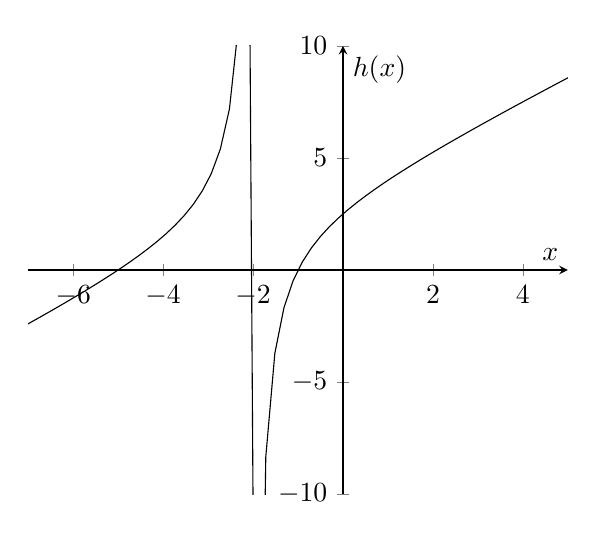
\begin{tikzpicture}
\begin{axis}[
    axis lines = center,
    xlabel = $x$,
    ylabel = $h(x)$,
    xmin = -7, xmax=5, ymin=-10, ymax=10
]
\addplot [
    domain=-10:10,
    samples=100, 
    color=black,
]
{(x^2+6*x+5)/(x+2)};
\end{axis}
\end{tikzpicture}
\]
The vertical line represents an \textbf{asymptote}, or a line which the graph can never reach. Let us examine the behavior of the above graph. First, there seems to be something interesting going on at $x=-2$. What happens when we get extremely close to $x=-2$ from the right side (the positive side)? What about the left side (the negative side)? We can create the following table:
\\
\\
\[\begin{tabular}{c|c}
    $x$ & $h(x)$ \\
    \hline
    $-3$ & $4$\\
    $-2.1$ & $31.9$\\
    $-2.01$ & $301.99$\\
    $-2.001$ & $3001.999$\\
    $-2$ & undefined\\
    $-1.999$ & $-2997.999$\\
    $-1.99$ & $-297.99$\\
    $-1.9$ & $-27.9$\\
    $-1$ & $0$\\
\end{tabular}\]
It seems that as we approach $x=-2$ from the left, the value of $h(x)$ increases without bound. On the other hand, when we approach $x=-2$ from the right, the value of $h(x)$ seems to decrease without bound. 
\\
\\
Let's think about why this might be true. Let $x<-2$ and $\left|x-(-2)\right|<\delta$, where $\delta$ is a \textit{very} small positive number. (It might be helpful to think of $\delta$ as $\delta=0.001$.) Essentially, we are saying that $x$ is a number that is \textit{super} close to $-2$, but still less than $-2$.
\\
\\
Then, the numerator of $h(x)$ is negative (this is because $x^2+6x+5$ is very close to $(-2)^2+6(-2)+5=-3<0$). The denominator is negative as well because if $x<-2$, then $x+2<-2+2=0$.
\\
\\
Therefore, when $x<-2$ and $\left|x-(-2)\right|<\delta$, 
\[h(x)=\frac{\text{negative number}}{\text{negative number}}=\text{positive number}.\]
Therefore, $h(x)>0$, and we can see this is true by examining the graph. Additionally, since $\left|x-(-2)\right|<\delta$, the denominator of $h(x)$ is \textit{extremely} small while the numerator stays close to $-3$. This means that $h(x)$ is not only positive, but it is \textit{very} large in magnitude. In fact, as $\delta$ becomes smaller and closer to 0, the value of $h(x)$ will grow without bound. 
\\
\\
What about when $x>-2$ and $\left|x-(-2)\right|<\delta$? In this case, $x$ is a number that is greater than 2, but only by a \textit{very} small amount. Then, the numerator is still close to $-3<0$, but the denominator is positive since $x>-2\to x+2>0$. Therefore, 
\[h(x)=\frac{\text{negative number}}{\text{positive number}}=\text{negative number}.\]
So, $h(x)<0$, and we can again see this is true by examining the graph. Additionally, since $\left|x-(-2)\right|<\delta$, the denominator of $h(x)$ is \textit{extremely} small (again). As such, $h(x)$ is a negative number with a very large magnitude. 
\\
\\
Before we go on, our use of \textit{extremely} and \textit{very} seems to be very ``hand wavy.'' Calculus gives us a way to represent these ideas through a \textbf{limit}. Let's explore this concept.
\\
\\
First, how do we represent $h(x)$ when $x<-2$ and $\left|x-(-2)\right|<\delta$? In other words, how do we represent the value of $h(x)$ where $x$ \textit{approaches} $-2$ but is still less than $-2$? We can use a limit, as follows:
\[\lim_{x\to -2^-} h(x).\]
Here, we are taking the ``limit'' as $x$ approaches $-2$ from the left  hand side (or the negative side) of $h(x)$. Take a moment to see how this matches up with the notation above. The arrow ($\to$) represents that $x$ is approaching $-2$ from the left hand side. In truth, $x$ will never \textit{be} $-2$, but the limit will ensure that we are using a value of $x$ that is \textit{extremely} close to the desired $-2$. 
\\
\\
Try doing the next case yourself.
\begin{problem}
How do we represent $h(x)$ when $x>-2$ and $\left|x-(-2)\right|<\delta$? In other words, how do we represent the value of $h(x)$ where $x$ \textit{approaches} $-2$ but is still greater than $-2$? Use a limit.
\end{problem}

The answer to this question is similar to the last limit:
\[\lim_{x\to -2^+} h(x).\]
However, there is one difference. We are approaching $-2$, but from the right hand side this time. So, we write a positive sign to the top right of $-2$ instead of the negative sign. Everything else is the same. 
\\
\\
We have our limit expressions. Now how do we evaluate them? Recall that The value of 
\[\lim_{x\to -2^-} h(x)\]
is positive and grows without bound. In Calculus, we represent quantities which grow without bound as $\infty$, pronounced ``infinity.'' $\infty$ is the highest theoretical number, but it is \textit{not} a number. It is a conceptual mechanism which allows us to think of arbitrarily large numbers.
\begin{remark}
Here is a word of caution: Do not say that $\infty$ is a number to a mathematician. Chances are, they will get angry. \Smiley
\end{remark}
The corresponding theoretical smallest negative number is $-\infty$. 
\\
\\
Therefore, we can say that 
\[\lim_{x\to -2^-} h(x)=\infty.\]
Similarly,
\[\lim_{x\to -2^+} h(x)=-\infty\]
because this limit grows without bound and is negative.
\\
\\
In this last example, we introduced the limit, a profound idea which separates Calculus from other branches of mathematics. Through this example, we got a glimpse as to how a limit works in practice, but we have yet to cover the rigorous definition of a limit. We will do this now.
\\
\\
\begin{remark}
Note that in the previous example, where the limits where $\infty$ and $-\infty$, the limits Do Not Exist (DNE). This is because $\infty$ is not a real number. We often write DNE as our answer, specifying that this limit Does Not Exist because it tends to $\infty$ or $-\infty$. 
\end{remark}
\subsubsection{Definition of a Limit}
Consider some function $f(x)$. Let's say we wish to examine the behavior of $f(x)$ as $x$ approaches $a$ from the right. Define $L$ as the limit of $f(x)$ as $x$ approaches $a$ from the right, or:
\[L=\lim_{x\to a^+} f(x).\]
What does this mean? Well, if $x$ approaches $a$ from the right, then $x>a\to x-a>0$. Additionally, $\left|x-a\right|$, or the distance between $x$ and $a$ on the number line, becomes extremely small when $x$ approaches $a$. Let $\delta$ be some number that we can choose such that
\[\left|x-a\right|<\delta.\]
\begin{remark}
Note that after we choose some $\delta$, which is usually a \textit{very} small positive number, we can simply produce a value of $x$ that is close enough to $a$. 
\end{remark}
Then, under the condition that $\left|x-a\right|<\delta$, we can choose some $\delta$ such that the value $\left|f(x)-L\right|$, or the distance between the limit $L$ and the value $f(x)$ on the number line, is substantially small. 
\\
\\
Let $\epsilon$ be some positive number ($\epsilon>0$). Therefore, \[0\leq\left|f(x)-L\right|<\epsilon\] 
for any value of $\epsilon$, no matter how small. 
\\
\\
But what does this mean? In English, this means that when $x$ approaches $a$, the distance between $f(x)$ and $L$ is so small that it is almost 0. In other words, as $x$ approaches $a$, $f(x)$ approaches $L$. 
\\
\\
Similarly, say we wished to evaluate 
\[L=\lim_{x\to a^-} f(x).\]
Then, $x<a\to x-a<0$. We must be able to choose some $\delta$ such that $\left|x-a\right|<\delta$ and $0\leq\left|f(x)-L\right|<\epsilon$. The only difference this time is that $x$ is approaching $a$ from the left instead of the right.
\\
\\
Now, define 
\[L_1=\lim_{x\to a^+} f(x)\]
and 
\[L_2=\lim_{x\to a^-} f(x).\]
If $L_1$ or $L_2$ is infinite, then that respective limit Does Not Exist (DNE). Otherwise, if $L_1=L_2$, let $L=L_1=L_2$. Then we define the following limit:
\[L=\lim_{x\to a} f(x).\]
On the other hand, if $L_1\neq L_2$, then the value
\[\lim_{x\to a} f(x)\]
Does Not Exist (DNE).
\\
\\
Essentially, if the limit of $f(x)$ as $x$ approaches $a$ from the right is the same as the limit of $f(x)$ as $x$ approaches $a$ from the left, then we can define the limit of $f(x)$ as $x$ approaches $a$ (without specifying from which direction).
\\
\\
If 
\[\lim_{x\to a^+} f(x)=\lim_{x\to a^-} f(x)=f(a),\]
then $f(x)$ is \textbf{continuous} at $x=a$. If we say a function is continuous, we often mean that the function is continuous over all points in its domain. 

\subsubsection{Examples of a Limit}
Let's do some practice problems to reinforce our knowledge of the limit. Try this problem on your own before seeing the solution.
\begin{problem}
Evaluate the following limit:
\[\lim_{x\to 5}\frac{x^2-25}{x^2-4x-5}.\]
\end{problem}
\paragraph{Solution} Let 
\[f(x)=\frac{x^2-25}{x^2-4x-5},\]
so we are trying to determine
\[\lim_{x\to 5} f(x).\]
First, we graph to see what we are working with:
\[
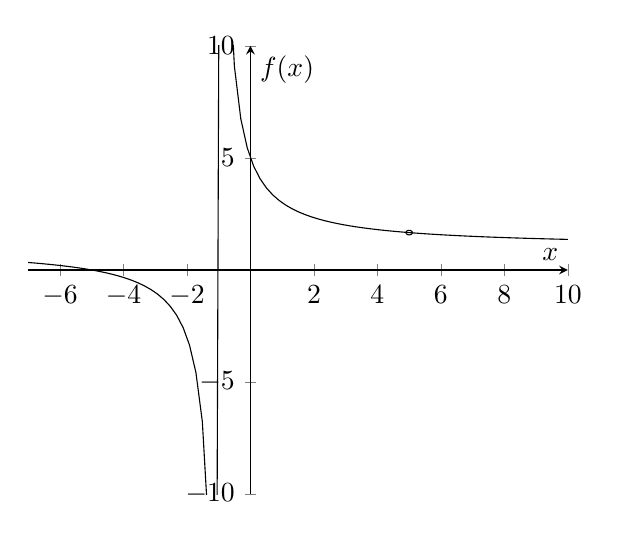
\begin{tikzpicture}
\begin{axis}[
    axis lines = center,
    xlabel = $x$,
    ylabel = $f(x)$,
    xmin = -7, xmax=10, ymin=-10, ymax=10
]
\addplot [
    domain=-10:10,
    samples=100, 
    color=black,
]
{(x^2-25)/(x^2-4*x-5)};
\addplot [
    domain=5.1:4.9,
    samples=100, 
    color=black,
]
{(1/100-(x-5)^2)^.5+5/3};
\addplot [
    domain=5.1:4.9,
    samples=100, 
    color=black,
]
{-(1/100-(x-5)^2)^.5+5/3};
\end{axis}
\end{tikzpicture}
\]
By definition, $f(x)$ is undefined when $x=-1$ and $x=5$. There is a vertical asymptote at $x=-1$, but we are more interested in the behavior at $x=5$. The graph seems to be approaching the same value from the left and right of $x=5$, but we have to make sure. 
\\
\\
First, we evaluate the limit as $x$ approaches 5 from the right:
\begin{align*}
    &\lim_{x\to 5^+} f(x)\\
    =&\lim_{x\to 5^+} \frac{x^2-25}{x^2-4x-5}\\
    =&\lim_{x\to 5^+} \frac{(x+5)(x-5)}{(x+1)(x-5)}\\
    =&\lim_{x\to 5^+} \frac{(x+5)\cancel{(x-5)}}{(x+1)\cancel{(x-5)}}\\
    =&\lim_{x\to 5^+} \frac{x+5}{x+1}\\
    =&\frac{5+5}{5+1}\\
    =&\frac{10}{6}\\
    =&\frac{5}{3}
\end{align*}
\\
\\
Notice that we can make the cancellation in the fraction above because $x-5\neq 0$. (Remember, even though $x$ is \textit{very} close to 5, it is \textit{not} 5. Therefore, $x-5$ is nonzero and we can make the cancellation.)
\\
\\
Now, we evaluate the limit as $x$ approaches 5 from the left:
\begin{align*}
    &\lim_{x\to 5^-} f(x)\\
    =&\lim_{x\to 5^-} \frac{x^2-25}{x^2-4x-5}\\
    =&\lim_{x\to 5^-} \frac{x+5}{x+1}\\
    =&\frac{5+5}{5+1}\\
    =&\frac{5}{3}
\end{align*}
Notice that the limits from the left and right were evaluated in almost the same way. Additionally, notice that 
\[\lim_{x\to 5^+} f(x)=\lim_{x\to 5^-} f(x).\]
Therefore, the value 
\[\lim_{x\to 5} f(x)\]
is defined as 
\[\lim_{x\to 5} f(x)=\lim_{x\to 5^+} f(x)=\lim_{x\to 5^-} f(x)=\frac{5}{3},\]
and this concludes the problem. 
$\boxed{}$\\
\\
We can see that even though $f(x)$ is not defined at $x=5$, we can find the limit as $x$ \textit{approaches} 5. Additionally, the value of $\frac{5}{3}$ seems to make sense when we look at the graph. Specifically, this limit value could be thought of as our ``prediction'' of what $f(x)$ would be if $f(x)$ was defined at $x=5$. 
\\
\\
Secondly, notice the way in which we evaluated the limit. We factored both the numerator and the denominator. We then canceled $x-5$ in the numerator and denominator, after which we plugged in 5 for $x$. Even though $x$ is not exactly 5, the expressions like $x+5$ are negligibly the same as if we used 5 for $x$. Can you see why?
\\
\\
\subsubsection{Properties of Limits}
Now, let's explore some common rules of limits. For these examples, $c$ is some constant and we have $x$ approaching some constant $a$. The functions $f(x)$ and $g(x)$ are some functions of $x$. Additionally, let 
\[L=\lim_{x\to a}f(x)\]
and 
\[K=\lim_{x\to a}g(x).\]
\paragraph{Constant Property of Limits} The following is a very simple limit rule, but it is still very important:
\[\lim_{x\to a} cf(x) = c\lim_{x\to a}f(x)=c\cdot L.\]
\paragraph{Proof} We know that (according to the definition of a limit), there is some value of $\delta>0$ such that $\left|x-a\right|<\delta$ and $0\leq\left|f(x)-L\right|<\epsilon$. Multiplying the latter inequality by $|c|$, we get:
\[0\leq|c|\cdot \left|f(x)-L\right|<|c|\cdot \epsilon.\]
Since $\epsilon$ is any positive number, we can choose its value so that $|c|\cdot \epsilon$ can be any positive number (since $c$ is constant). Therefore, we can simplify the expression by replacing $|c|\cdot \epsilon$ with the simpler $\epsilon$. Additionally, we can make the following simplification:
\[|c|\cdot \left|f(x)-L\right|= \left|c\cdot f(x)-c\cdot L\right|.\]
Then, we can safely claim the following statement: there is some value of $\delta>0$ such that $|x-a|>0$ and $0\leq\left|c\cdot f(x)-c\cdot L\right|<\epsilon$. This statement is equivalent to the following equality:
\[\lim_{x\to a} c\cdot f(x)=c\cdot L.\]
Therefore,
\[\lim_{x\to a} cf(x) = c\lim_{x\to a}f(x)=c\cdot L.\text{ }\boxed{}\]
\\
\\
A specific case of this rule occurs when $f(x)=x$. If this is the case, then the rule reads:
\[\lim_{x\to a} c\cdot x = c\lim_{x\to a}x=c\cdot a\]
if $a$ is not infinite.
\\
\\
Another specific case of this rule occurs when $f(x)=1$. In this case, the rule reads:
\[\lim_{x\to a} c\cdot 1 = c\lim_{x\to a}1=c\cdot 1 = c\]
if $a$ is not infinite. Another way to think about this limit property is to realize that the value of $c$ is not dependent on the value of $x$ because $c$ is constant. 
\paragraph{Addition Property of Limits} Next is the Addition Property of limits:
\[\lim_{x\to a}[f(x)+g(x)]=\lim_{x\to a}f(x) + \lim_{x\to a}g(x)=L+K.\]

\paragraph{Proof} We know that there exists some $\delta_1>0$ such that $\left|x-a\right|<\delta_1$ and $0\leq\left|f(x)-L\right|<\epsilon$.
\\
\\
Similarly, there exists some $\delta_2>0$ such that $\left|x-a\right|<\delta_2$ and $0\leq\left|g(x)-K\right|<\epsilon$.
\\
\\
We can add the two latter inequalities to get:
\[0\leq \left|f(x)-L\right| + \left|g(x)-K\right| < 2\epsilon.\]
Recall the Triangle Inequality (from Geometry or Algebra), which states the following:
\[|w|+|z|\geq |w+z|\]
for any numbers $w$ and $z$ (this property holds for all complex numbers). Therefore, 
\[\left|f(x)-L\right| + \left|g(x)-K\right| \geq \left|f(x)-L + g(x)-K\right|=\left|(f(x) + g(x))-(L+K)\right|.\]
Combining this from the statement from before, we find that 
\[0\geq \left|(f(x) + g(x))-(L+K)\right|\leq \left|f(x)-L\right| + \left|g(x)-K\right| < 2\epsilon.\]
Noting that $2\epsilon$ is some positive number, we find that $2\epsilon$ can be replaced with the simpler $\epsilon$. Then, simplifying this, we get
\[0\geq \left|(f(x) + g(x))-(L+K)\right| < \epsilon.\]
Now, let $\delta=\min(\delta_1,\delta_2)$. Recall the initial conditions $|x-a|<\delta_1$ and $|x-a|<\delta_2$. Note that with the new value of $\delta$, both of these initial conditions are satisfied. (Why?)
\\
\\
Putting these two new conditions together, we can claim: there is some value of $\delta >0$ such that $|x-a|<\delta$ and $0\geq \left|(f(x) + g(x))-(L+K)\right| < \epsilon$. This statement translates to the following equality: 
\[\lim_{x\to a} [f(x)+g(x)]=L+K.\]
In other words, 
\[\lim_{x\to a}[f(x)+g(x)]=\lim_{x\to a}f(x) + \lim_{x\to a}g(x)=L+K.\text{ }\boxed{}\]

\paragraph{Subtraction Property of Limits} Very similar to the Addition Property of limits is the Subtraction Property of limits:
\[\lim_{x\to a}[f(x)-g(x)]=\lim_{x\to a}f(x) - \lim_{x\to a}g(x)=L-K.\]
\begin{problem}
The proof for the Subtraction Property is very similar to the Addition Property. Can you prove it? (Hint: Remember to use the Triangle Inequality.) 
\\
\\
Besides proving from scratch, another method to proving the Subtraction Property is to use the Constant Property and the Addition Property together. Concretely, evaluate the following limit:
\[\lim_{x\to a}[f(x)+c\cdot g(x)],\]
where $c=-1$. (How does this relate to the Subtraction Property?)
\end{problem}

\paragraph{Multiplication Property of Limits} The Multiplication Property of limits states the following:
\[\lim_{x\to a}[f(x)\cdot g(x)]=\lim_{x\to a}f(x) \cdot \lim_{x\to a}g(x)=L\cdot K.\]

\paragraph{Proof} Again, we return to the definition of a limit:
\\
\\
We know that there exists some $\delta_1>0$ such that $\left|x-a\right|<\delta_1$ and $0\leq\left|f(x)-L\right|<\epsilon$.
\\
\\
Similarly, there exists some $\delta_2>0$ such that $\left|x-a\right|<\delta_2$ and $0\leq\left|g(x)-K\right|<\epsilon$.
\\
\\
Let's rewrite these two statements in a slightly different way:
\\
\\
We know that there exists some $\delta_1>0$ such that $\left|x-a\right|<\delta_1$ and $0\leq\left|(f(x)-L)-0\right|<\epsilon$.
\\
\\
This statement translates to the following equality:
\[\lim_{x\to a} [f(x)-L] = 0.\]
\\
\\
Similarly, there exists some $\delta_2>0$ such that $\left|x-a\right|<\delta_2$ and $0\leq\left|(g(x)-K)-0\right|<\epsilon$.
\\
\\
This statement translates to the following equality:
\[\lim_{x\to a} g(x)-K = 0.\]
Multiplying the latter inequalities together, we get the following:
\[0\leq\left|(f(x)-L)-0\right|\cdot \left|(g(x)-K)-0\right|<\epsilon\]
or 
\[0\leq\left|(f(x)-L)(g(x)-K)-0\right|<\epsilon.\]
Let $\delta=\min(\delta_1,\delta_2)$ and $|x-a|<\delta$, like before.
\\
\\
Then, these two combine to give us the following equality:
\[\lim_{x\to a} (f(x)-L)(g(x)-K) = 0.\]
\\
\\
This fact will be necessary for our proof. Let's expand the following product:
\[[f(x)-L]\cdot [g(x)-K] = f(x)\cdot g(x) - K\cdot f(x) - L\cdot g(x) + LK.\]
Rearranging this, we get the following:
\[f(x)\cdot g(x) = [f(x)-L]\cdot [g(x)-K] + K\cdot f(x) + L\cdot g(x) - LK.\]
We now take the limit as $x$ approaches $a$ on both sides and simplify (take note of this technique where we take the limit of both sides of an equation):
\begin{align*}
    \lim_{x\to a} f(x)\cdot g(x) &= \lim_{x\to a} \left([f(x)-L]\cdot [g(x)-K] + K\cdot f(x) + L\cdot g(x) - LK\right) \\
    \lim_{x\to a} f(x)\cdot g(x) &= \lim_{x\to a} \left([f(x)-L]\cdot [g(x)-K]\right) + \lim_{x\to a} K\cdot f(x) + \lim_{x\to a} L\cdot g(x) - \lim_{x\to a} LK \\
    \lim_{x\to a} f(x)\cdot g(x) &= \lim_{x\to a} \left([f(x)-L]\cdot [g(x)-K]\right) + K\cdot \lim_{x\to a} \cdot f(x) + L\cdot \lim_{x\to a} \cdot g(x) - LK \\
    \lim_{x\to a} f(x)\cdot g(x) &= \lim_{x\to a} \left([f(x)-L]\cdot [g(x)-K]\right) + K\cdot L + L\cdot K - LK \\
    \lim_{x\to a} f(x)\cdot g(x) &= \lim_{x\to a} \left([f(x)-L]\cdot [g(x)-K]\right) + LK \\
    \lim_{x\to a} f(x)\cdot g(x) &= \lim_{x\to a} \left([f(x)-L]\cdot [g(x)-K]\right) + LK \\
    \lim_{x\to a} f(x)\cdot g(x) &= 0 + LK \\
\end{align*}
\\
Notice how we use our previous rules in each of the steps. Therefore, 
\[\lim_{x\to a} f(x)\cdot g(x) = LK.\]
In conclusion,
\[\lim_{x\to a}[f(x)\cdot g(x)]=\lim_{x\to a}f(x) \cdot \lim_{x\to a}g(x)=L\cdot K.\text{ }\boxed{}\]

\paragraph{Division Property of Limits} The Division Property of limits states the following:
\[\lim_{x\to a}\frac{f(x)}{g(x)}=\frac{\lim_{x\to a}f(x)}{\lim_{x\to a}g(x)}=\frac{L}{K}\]
as long as $K=\lim_{x\to a} g(x)\neq 0$ (otherwise we would be doing division by 0).
\paragraph{Proof} In the proof of the Division Property, we use the Multiplication Property, which we already proved. Specifically,
\[\lim_{x\to a}\frac{f(x)}{g(x)}=\lim_{x\to a}f(x)\cdot \frac{1}{g(x)}=\lim_{x\to a}f(x)\cdot \lim_{x\to a} \frac{1}{g(x)}.\]
We will be done if we can prove the following:
\[\lim_{x\to a} \frac{1}{g(x)} = \frac{1}{\lim_{x\to a} g(x)}.\]
Do you see why? 
\\
\\
We know that we can pick some $\delta_1>0$ such that $|x-a|<\delta_1$ and 
\[0\leq |g(x)-K|<\epsilon\]
for any $\epsilon>0$. For this proof, we will do something different. We will pick a specific value for $\epsilon$. Note that we can do this as long as the value we pick is positive (because $\epsilon$ can be any positive number). 
\\
\\
Let $\epsilon=\frac{|K|}{2}>0$. Therefore, the final condition becomes 
\[0\leq |g(x)-K|<\frac{|K|}{2}.\tag{$*$}\]
Now, we apply the Triangle Inequality once again to develop another useful equality:
\begin{align*}
    |K| &= |K-g(x)+g(x)|\\
    &\leq |K-g(x)| + |g(x)|\\
    &\leq |g(x)-K| + |g(x)|\\
    &< \frac{|K|}{2} + |g(x)|,
\end{align*}
\\
where we applied inequality $(*)$ in the last step. Subtracting $\frac{|K|}{2}$ from both sides of this inequality, we get:
\[\frac{|K|}{2}<|g(x)|.\]
Taking the reciprocal of both sides (and switching the inequality sign as per the rules of inequalities), we get the following inequality:
\[\frac{2}{|K|}>\frac{1}{|g(x)|}.\tag{$\triangle$}\]
Now, we will perform a similar argument again. Specifically, we know that we can pick some $\delta_2>0$ such that $|x-a|<\delta_2$ and 
\[0\leq |g(x)-K|<\epsilon\]
for any $\epsilon>0$. We will once again choose a specific value for $\epsilon$. This time, let $\epsilon=\frac{|K|^2}{2}\cdot \epsilon_1$ for some $\epsilon_1>0$. So, 
\[0\leq |g(x)-K|<\frac{|K|^2}{2}\cdot \epsilon_1.\tag{$\diamond$}\]
\\
\\
Now, let $\delta=\min(\delta_1,\delta_2)$ so that both of our prior inequalities are satisfied. (We have done this a few times now. Make sure you understand why this method works.) 
\\
\\
Now, time for some algebra:
\begin{align*}
    \left|\frac{1}{g(x)}-\frac{1}{K}\right|&=\left|\frac{K-g(x)}{g(x)\cdot K}\right|\\
    &= \frac{1}{|g(x)|}\cdot \frac{1}{|K|}\cdot \left|g(x)-K\right|\\
    &< \frac{2}{|K|}\cdot \frac{1}{|K|}\cdot \frac{|K|^2}{2}\cdot \epsilon_1\tag{3}\\
    &< \epsilon_1,
\end{align*}
\\
where we used $(\triangle)$ and $(\diamond)$ in step $(3)$. Therefore, we are left with the following statement: we can choose some $\delta>0$ such that $|x-a|<\delta$ and 
\[0\leq \left|\frac{1}{g(x)}-\frac{1}{K}\right|< \epsilon_1,\]
where $\epsilon_1$ is any positive number. Seem familiar? It should because this translates to the following limit:
\[\lim_{x\to a} \frac{1}{g(x)} = \frac{1}{K}=\frac{1}{\lim_{x\to a} g(x)},\]
as desired. As mentioned before, we can use this property along with the Product Property of limits, which we proved before, to prove the Division Property of limits. 
$\boxed{}$

\subsection{Derivatives}
In this section, we will look at an important subset of limits: the \textbf{derivative}. The idea of a derivative will help us learn more about the ``slope of the tangent line'' we were after in the first place. 

\subsubsection{Definition of a Derivative}
First, we start with the definition of a derivative. Let $f(x)$ be some function. The derivative of $f(x)$ is represented by $f'(x)$, $\diff{f(x)}{x}$, or $\diff{}{x}f(x)$. For the last two, the $dx$ represents that we are taking the derivative of $f(x)$ with respect to the variable $x$. Then, the definition of the derivative is the following:
\[\diff{f(x)}{x}=\lim_{h\to 0}\frac{f(x+h)-f(x)}{(x+h)-x}=\lim_{h\to 0}\frac{f(x+h)-f(x)}{h}.\]
Let $a=x+h$. Then, the condition $\lim_{h\to 0}$ is the same as $\lim_{x\to a}$. Do you see why? Then, the definition the derivative becomes:
\[\diff{f(x)}{x}=\lim_{x\to a}\frac{f(a)-f(x)}{a-x}.\]
Both of these expressions are valid definitions of the derivative. As you may expect, we say that the derivative as $x$ approaches $a$ from the left (or as $h$ approaches 0 from the left) is the following:
\[\diff{f(x)}{x}=\lim_{x\to a^-}\frac{f(a)-f(x)}{a-x}=\lim_{h\to 0^-}\frac{f(x+h)-f(x)}{h}.\]
Similarly, we say that the derivative as $x$ approaches $a$ from the right (or as $h$ approaches 0 from the right) is the following:
\[\diff{f(x)}{x}=\lim_{x\to a^+}\frac{f(a)-f(x)}{a-x}=\lim_{h\to 0^+}\frac{f(x+h)-f(x)}{h}.\]
The derivative is only defined if the derivative from the left and right exist and are equal. 

\subsubsection{Interpretation of a Derivative}
We have the definition of a derivative, but what does this mean? Is there any significance to this definition?
\\
\\
The answer is yes. The derivative is the ``slope of the tangent line.'' Take a look at the second definition of the derivative:
\[\diff{f(x)}{x}=\lim_{x\to a}\frac{f(a)-f(x)}{a-x}.\]
Do you see anything familiar here? This fraction is 
\[\frac{\text{change in $y$-values}}{\text{change in $x$-values}}.\]
In other words, this value represents the slope of the line going through two different points. Which points? Looking back at the definition, we see that the derivative is the slope of the line going through $(a,f(a))$ and $(x,f(x))$. Since $x$ approaches $a$, the two points are very close to each other.

\webfig{idl-derivative}


\subsubsection{Derivatives Examples}
Let's try some examples to get a better sense of how derivatives work. 
\\
\\
\begin{problem}
Let $f(x)=2x+1$. Evaluate $\diff{f(x)}{x}$ when $x=5$.
\end{problem}
\paragraph{Solution} Using the first definition of the derivative, we get the following expression:
\begin{align*}
    \diff{f(x)}{x}&=\lim_{h\to 0}\frac{f(x+h)-f(x)}{h}\\
    &=\lim_{h\to 0}\frac{2(x+h)+1-(2x+1)}{h}\\
    &=\lim_{h\to 0}\frac{2x+2h+1-2x-1}{h}\\
    &=\lim_{h\to 0}\frac{2h}{h}\\
    &=2.
\end{align*}
Remember in the last step that while $h$ approaches 0, it is never exactly 0. Therefore, we can make this simplification. Therefore, $\diff{f(x)}{x}=2$ no matter what $x$ is! In other words, the slope of the tangent line to $f(x)$ is always 2. This makes sense when we look at the following graph of $f(x)$:
\[
\begin{tikzpicture}
\begin{axis}[
    axis lines = center,
    xlabel = $x$,
    ylabel = $f(x)$,
    xmin = -7, xmax=10, ymin=-10, ymax=10
]
\addplot [
    domain=-10:10,
    samples=100, 
    color=black,
]
{2*x+1};
\end{axis}
\end{tikzpicture}
\]
Because $f(x)$ is a line, it makes sense that the slope is constant over all real numbers. Therefore, the slope at $x=5$ (or any other $x$-value for that matter) is 2. $\boxed{}$
\\
\\
What about when the slope is not the same over the whole domain? Consider the following problem.
\begin{problem}
Let $f(x)=x^2+2x+3$. Evaluate $\diff{f(x)}{x}$ when $x=5$.
\end{problem}
\paragraph{Solution} Once again, we use the definition of the derivative to get the following expression:
\begin{align*}
    \diff{f(x)}{x}&=\lim_{h\to 0}\frac{f(x+h)-f(x)}{h}\\
    &=\lim_{h\to 0}\frac{(x+h)^2+2(x+h)+3-(x^2+2x+3)}{h}\\
    &=\lim_{h\to 0}\frac{x^2+h^2+2xh+2x+2h+3-x^2-2x-3}{h}\\
    &=\lim_{h\to 0}\frac{h^2+2xh+2h}{h}\\
    &=\lim_{h\to 0}h+2x+2\\
    &=2x+2.
\end{align*}
In the last step, we used the fact that $h$ is a number which is very close to 0. Therefore, $h+k=k$ for any $k$. 
\\
\\
We plug in $x=5$ to get our final answer because this is the condition given in the problem statement: $2x+2=2(5)+2=12$. Therefore, the slope of the tangent line to the graph of $f(x)$ at $(5,f(5))=(5,38)$ is 12.
\\
\\
We can actually go a step further and find the \textit{equation} of the tangent line at $x=5$. We know a point through which the line passes, namely $(5,38)$, and the slope of the line, which is 12. We can then use the point slope form of a line to find it's equation:
\[y-38=12(x-5).\]
In the following graph, we plot $f(x)$ and the tangent line to the graph at $x=5$:
\[
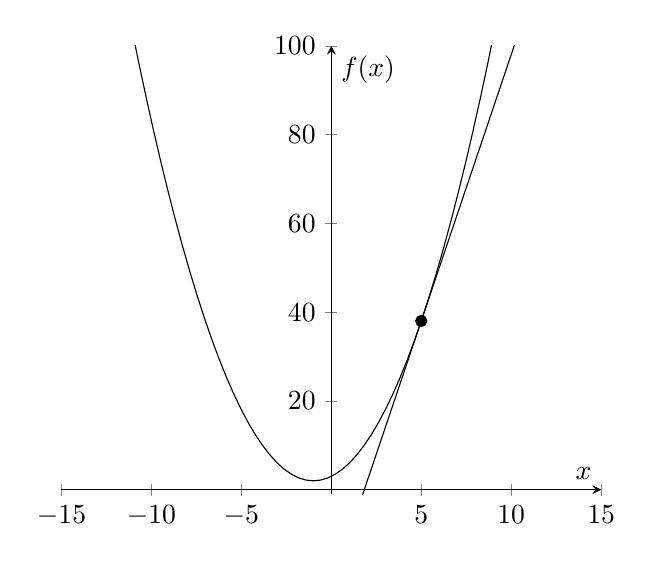
\begin{tikzpicture}
\begin{axis}[
    axis lines = center,
    xlabel = $x$,
    ylabel = $f(x)$,
    xmin = -15, xmax=15, ymin=-1, ymax=100
]
\addplot [
    domain=-20:20,
    samples=100, 
    color=black,
]
{x^2+2*x+3};
\addplot [
    domain=-20:20,
    samples=100, 
    color=black,
]
{12*x-22};
\addplot[mark=*] coordinates {(5,  38)};
\end{axis}
\end{tikzpicture}
\]
In fact, using the formula we derived for the derivative of $f(x)$, we can find the slope of the tangent line (derivative) at any point in the domain of $f(x)$. Using the point $(x,f(x))$ and this slope, we can also find the equation of the tangent line at any point in the domain of $f(x)$. 
\\
\\
Notice one more thing: the slope of the tangent line is not the same over the whole domain of $f(x)$ as it was in the last problem. Instead, it depends on the value of $x$, which should make sense looking at the graph. $\boxed{}$

\subsubsection{Properties of Derivatives}
As you may have guessed, derivatives have several important properties. In this section, we will state and prove these properties. You will see how we use the definition of the derivative along with the limit properties we proved in the last section to complete these proofs.
\\
\\
In this section, we will be taking the general derivative of a function. Specifically, we will not be finding the derivative at any one point $x=a$, but rather for some general $x$ in the domain of the function. 
\\
\\
Additionally, we will assume that $f(x)$ and $g(x)$ are functions such that $\diff{f(x)}{x}$ and $\diff{g(x)}{x}$ are both defined for all $x$ which are in the domains of both $f(x)$ and $g(x)$. Finally, let $c$ be some constant.

\paragraph{Constant Property of Derivatives} The Constant Property of derivatives states the following:
\[\diff{(c\cdot f(x))}{x}=c\cdot \diff{f(x)}{x}.\]

\paragraph{Proof} Starting with the right side and the definition of the derivative, we get the following expression (and prove the property):
\[c\cdot \diff{f(x)}{x}=c\cdot \lim_{h\to 0}\frac{f(x+h)-f(x)}{h}=\lim_{h\to 0}\frac{c\cdot f(x+h)-c\cdot f(x)}{h}=\diff{(c\cdot f(x))}{x}.\text{ }\boxed{}\]

\paragraph{Addition Property of Derivatives} The Addition Property of derivatives states the following: 
\[\diff{f(x)}{x}+\diff{g(x)}{x}=\diff{[f(x)+g(x)]}{x}.\]

\paragraph{Proof} We start with the left side and use the definition of the derivative to derive the following expression:
\begin{align*}
    &\diff{f(x)}{x}+\diff{g(x)}{x}\\
    =&\lim_{h\to 0}\frac{f(x+h)-f(x)}{h} + \lim_{h\to 0}\frac{g(x+h)-g(x)}{h}\\
    =&\lim_{h\to 0}\left[\frac{f(x+h)-f(x)}{h} + \frac{g(x+h)-g(x)}{h}\right]\tag{2}\\
    =&\lim_{h\to 0}\left[\frac{f(x+h)-f(x)+g(x+h)-g(x)}{h}\right]\\
    =&\lim_{h\to 0}\left[\frac{[f(x+h)+g(x+h)]-[f(x)+g(x)]}{h}\right]\\
    =&\diff{[f(x)+g(x)]}{x}.
\end{align*}
Notice how we used the Addition Property of limits in step (2). $\boxed{}$

\paragraph{Subtraction Property of Derivatives} The Subtraction Property of derivatives states the following:
\[\diff{f(x)}{x}-\diff{g(x)}{x}=\diff{[f(x)-g(x)]}{x}.\]

\begin{problem}
Try to prove the Subtraction Property from scratch as we did in the last proof.
\end{problem}

\paragraph{Proof} We will take an easier route this time, taking advantage of the Addition Property we just proved. Let $p(x)=-g(x)$. Then, we wish to prove the following statement: 
\[\diff{f(x)}{x}-\diff{(-p(x))}{x}=\diff{[f(x)+p(x)]}{x}.\]
Note that 
\[-\diff{(-p(x))}{x}=-\lim_{h\to 0}\frac{-p(x+h)+p(x)}{h}=\lim_{h\to 0}\frac{p(x+h)-p(x)}{h}=\diff{p(x)}{x}.\]
Therefore, the statement we wish to prove becomes 
\[\diff{f(x)}{x}+\diff{p(x)}{x}=\diff{[f(x)+p(x)]}{x},\]
which is true by the Addition Property of derivatives. Thus, we have proved our original statement, which was the Subtraction Property of derivatives. $\boxed{}$

\paragraph{Multiplication Property of Derivatives} The Multiplication Property of derivatives states the following:
\[\diff{[f(x)\cdot g(x)]}{x}=\diff{f(x)}{x}\cdot g(x) + f(x)\cdot \diff{g(x)}{x}.\]

\paragraph{Proof} We start with the left hand side and use the limit definition of a derivative to get the following expression:
\begin{align*}
    \diff{[f(x)\cdot g(x)]}{x} =&\lim_{h\to 0}\frac{f(x+h)\cdot g(x+h)-f(x)\cdot g(x)}{h}\\
    =&\lim_{h\to 0}\frac{f(x+h)\cdot g(x+h)-f(x+h)\cdot g(x)+f(x+h)\cdot g(x)-f(x)\cdot g(x)}{h}\\
    =&\lim_{h\to 0}\frac{f(x+h)\cdot [g(x+h)-g(x)]+g(x)[f(x+h)-f(x)]}{h}\\
    =&\lim_{h\to 0}\frac{f(x+h)\cdot [g(x+h)-g(x)]}{h}+\lim_{h\to 0}\frac{g(x)[f(x+h)-f(x)]}{h}\\
    =&f(x)\cdot \lim_{h\to 0}\frac{g(x+h)-g(x)}{h}+g(x)\cdot \lim_{h\to 0}\frac{f(x+h)-f(x)}{h}\\
    =&f(x)\cdot \diff{g(x)}{x}+g(x)\cdot \diff{f(x)}{x}\\
    =&f(x)\cdot \diff{g(x)}{x}+\diff{f(x)}{x}\cdot g(x)\\
    =&\diff{f(x)}{x}\cdot g(x) + f(x)\cdot \diff{g(x)}{x}.
\end{align*}
Hence, we have proved the Multiplication Property of derivatives. $\boxed{}$

\paragraph{Division Property of Derivatives} The Division Property of derivatives states the following:
\[\diff{[f(x) / g(x)]}{x}=\frac{\diff{f(x)}{x}\cdot g(x) - f(x)\cdot \diff{g(x)}{x}}{(g(x))^2}.\]

\paragraph{Proof} We start with the left side and use the limit definition of a derivative to get our answer: 
\begin{align*}
    \diff{[f(x) / g(x)]}{x} &= \lim_{h\to 0}\frac{\frac{f(x+h)}{g(x+h)}-\frac{f(x)}{g(x)}}{h}\\
    &= \lim_{h\to 0}\frac{f(x+h)\cdot g(x) - f(x)\cdot g(x+h)}{g(x)\cdot g(x+h)\cdot h}\\
    &= \lim_{h\to 0}\frac{1}{g(x)\cdot g(x+h)}\cdot \lim_{h\to 0}\frac{f(x+h)\cdot g(x) - f(x)\cdot g(x) + f(x)\cdot g(x) - f(x)\cdot g(x+h)}{h}\\
    &= \frac{1}{(g(x))^2}\cdot \left[\lim_{h\to 0}\frac{g(x) [f(x+h) - f(x)]}{h} - \lim_{h\to 0}\frac{f(x)[g(x+h) - g(x)]}{h}\right]\\
    &= \frac{1}{(g(x))^2}\cdot \left[g(x)\cdot \lim_{h\to 0}\frac{[f(x+h) - f(x)]}{h} - f(x)\cdot \lim_{h\to 0}\frac{[g(x+h) - g(x)]}{h}\right]\\
    &= \frac{1}{(g(x))^2}\cdot \left[g(x)\cdot \diff{f(x)}{x} - f(x)\cdot \diff{g(x)}{x}\right]\\
    &= \frac{\diff{f(x)}{x}\cdot g(x) - f(x)\cdot \diff{g(x)}{x}}{(g(x))^2}.\text{ }\boxed{}\\
\end{align*}

\paragraph{Chain Rule for Derivatives} If $f(x)$ and $g(x)$ are differentiable functions (meaning that we can take their derivatives), the Chain Rule for derivatives states the following:
\[\diff{f(g(x))}{x}=\diff{f(g(x))}{g(x)}\cdot \diff{g(x)}{x}.\]

\paragraph{Proof} We split our proof into two cases: \textbf{Case 1} occurs when $g(x+h)-g(x)$ \textit{approaches} 0 as $h$ approaches 0; \textbf{Case 2} occurs when $g(x+h)-g(x)$ \textit{equals} 0 as $h$ approaches 0. Notice how these two are different.

\paragraph{Case 1} For \textbf{Case 1}, we start with the left side and use the limit definition of a derivative to get the following expression:
\begin{align*}
    &\lim_{h\to 0}\frac{f(g(x+h))-f(g(x))}{h}\\
    =& \lim_{h\to 0}\left[\frac{f(g(x+h))-f(g(x))}{g(x+h)-g(x)}\cdot \frac{g(x+h)-g(x)}{h}\right]\\
    =& \lim_{h\to 0}\frac{f(g(x+h))-f(g(x))}{g(x+h)-g(x)}\cdot \lim_{h\to 0}\frac{g(x+h)-g(x)}{h}\\
    =& \lim_{h\to 0}\frac{f(g(x+h))-f(g(x))}{g(x+h)-g(x)}\cdot \diff{g(x)}{x}\\
    =& \lim_{h\to 0}\frac{f(g(x+h))-f(g(x))}{g(x+h)-g(x)}\cdot \diff{g(x)}{x}.
\end{align*}
Now, let $k=g(x+h)-g(x)$. Then, $g(x+h)=g(x)+k$. Note that by the definition of $k$, 
\[\lim_{h\to 0}g(x+h)-g(x)=0\to \lim_{h\to 0}k=0.\]
Therefore, the condition $\lim_{h\to 0}$ is equivalent to the condition $\lim_{k\to 0}$. Then, our expression becomes: 
\begin{align*}
    &\lim_{h\to 0}\frac{f(g(x+h))-f(g(x))}{g(x+h)-g(x)}\cdot \diff{g(x)}{x}\\
    =& \lim_{k\to 0}\frac{f(g(x)+k)-f(g(x))}{g(x)+k-g(x)}\cdot \diff{g(x)}{x}\\
    =& \lim_{k\to 0}\frac{f(g(x)+k)-f(g(x))}{k}\cdot \diff{g(x)}{x}\\
    =& \diff{f(g(x))}{g(x)}\cdot \diff{g(x)}{x}.
\end{align*}
This is equivalent to the right side, so we are done with \textbf{Case 1}.

\paragraph{Case 2} When $g(x+h)-g(x)=0$, $g(x)=g(x+h)$. Let $k=g(x)=g(x+h)$, where $k$ is constant in this case. This means, in words, that $k=g(a)$ for values of $a$ which are very close to $x$. Therefore, the graph of $g(x)$ around $x$ is a flat line. 
\\
\\
Now, let's take a look at the Chain Rule again:
\[\diff{f(g(x))}{x}=\diff{f(g(x))}{g(x)}\cdot \diff{g(x)}{x}.\]
Since $g(x)=k$ for values around $x$, the left side becomes:
\[\diff{f(g(x))}{x}=\diff{f(k)}{x}.\]
The right side becomes
\begin{align*}
    &\diff{f(g(x))}{g(x)}\cdot \diff{g(x)}{x}\\
    =&\diff{f(k)}{k}\cdot \diff{k}{x}\\
    =&\diff{f(k)}{k}\cdot \lim_{h\to 0}\frac{h}{h}\\
    =&\diff{f(k)}{k}\cdot 1\\
    =&\diff{f(k)}{k}.
\end{align*}
Therefore, the left and right side are equivalent, and \textbf{Case 2} has also been proved. 
\\
\\
Thus, we have proved the Chain Rule for derivatives. $\boxed{}$

\begin{remark}
Notice how the Chain Rule for derivatives looks like a cancellation of fractions. This is actually true to some extent. 
\\
\\
Remember that $\diff{f(x)}{x}$ is the slope of the tangent line to $f(x)$ at $x$. Recall from Algebra class that the slope of a line is computed using the following formula:
\[\frac{\text{change in $y$}}{\text{change in $x$}}=\frac{\Delta y}{\Delta x}.\]
One can think of $df(x)$ as $\Delta f(x)$ and $dx$ as $\Delta x$. Thinking of $df(x)$, etc. as a (very small) number (and not just notation) is actually central to solving Differential Equations, another Calculus concept (which we will not cover here). Using this idea, it is quite simple to remember the Chain Rule for derivatives.
\end{remark}

\subsubsection{Derivatives of Common Functions}
In this section, we will take a look at the derivatives of some commonly used functions in Calculus. Using these derivative ``rules'' along with our derivative properties and the Chain Rule for derivatives, we can take the derivative of most functions.
\\
\\
In these examples, $f(x)$ will be the function which we wish to take the derivative of and $c$ is some constant.

\paragraph{Power Rule} The Power Rule states: 
\[\diff{\left[x^c\right]}{x}=c\cdot x^{c-1}.\]

\paragraph{Proof} We use the limit definition of the derivative:
\begin{align*}
    &\lim_{h\to 0}\frac{f(x+h)-f(x)}{h}\\
    =&\lim_{h\to 0}\frac{(x+h)^c-x^c}{h}\\
    =&\lim_{h\to 0}\frac{\sum_{i=0}^{c}\left[\binom{c}{i}x^{c-i}h^i\right]-x^c}{h}\tag{2}\\
    =&\lim_{h\to 0}\frac{\binom{c}{0}x^{c-0}h^0+\binom{c}{1}x^{c-1}h^1+\sum_{i=2}^{c}\left[\binom{c}{i}x^{c-i}h^i\right]-x^c}{h}\\
    =&\lim_{h\to 0}\frac{x^c+c\cdot x^{c-1}h+h^2\cdot \sum_{i=2}^{c}\left[\binom{c}{i}x^{c-i}h^{i-2}\right]-x^c}{h}\\
    =&\lim_{h\to 0}\frac{c\cdot x^{c-1}h+h^2\cdot \sum_{i=2}^{c}\left[\binom{c}{i}x^{c-i}h^{i-2}\right]}{h}\\
    =&\lim_{h\to 0}\left[c\cdot x^{c-1}+h\cdot \sum_{i=2}^{c}\left[\binom{c}{i}x^{c-i}h^{i-2}\right]\right]\\
    =&c\cdot x^{c-1}+0\\
    =&c\cdot x^{c-1}.
\end{align*}
Thus, we are done. Note how we used the Binomial Theorem on line (2). $\boxed{}$

Now, we will state some derivatives of common functions without proving them because these are a bit more advanced for our purposes.

\paragraph{Derivative of $e^x$}
\[\diff{\left[e^x\right]}{x}=e^x.\]

\paragraph{Derivative of $c^x$}
\[\diff{\left[c^x\right]}{x}=\ln(c)\cdot c^x.\]

\paragraph{Derivative of $\ln(x)$}
\[\diff{\left[\ln(x)\right]}{x}=\frac{1}{x}.\]

\paragraph{Derivative of $\log_{c}(x)$}
\[\diff{\left[\log_{c}(x)\right]}{x}=\frac{1}{\ln(c)}\cdot \frac{1}{x}.\]

\paragraph{Derivative of $\sin(x)$}
\[\diff{\left[\sin(x)\right]}{x}=\cos(x)\]

\paragraph{Derivative of $\cos(x)$}
\[\diff{\left[\cos(x)\right]}{x}=-\sin(x)\]

\paragraph{Derivative of $\tan(x)$}
\[\diff{\left[\tan(x)\right]}{x}=\sec^2(x)\]

\paragraph{Derivative of $\sec(x)$}
\[\diff{\left[\sec(x)\right]}{x}=\tan(x)\cdot \sec(x)\]

\paragraph{Derivative of $\cot(x)$}
\[\diff{\left[\cot(x)\right]}{x}=-\csc^2(x)\]

\paragraph{Derivative of $\csc(x)$}
\[\diff{\left[\csc(x)\right]}{x}=-\cot(x)\cdot \csc(x)\]

\paragraph{Derivative of $\sin^{-1}(x)$}
\[\diff{\left[\sin^{-1}(x)\right]}{x}=\frac{1}{\sqrt{1-x^2}}\]

\paragraph{Derivative of $\cos^{-1}(x)$}
\[\diff{\left[\cos^{-1}(x)\right]}{x}=-\frac{1}{\sqrt{1-x^2}}\]

\paragraph{Derivative of $\tan^{-1}(x)$}
\[\diff{\left[\tan^{-1}(x)\right]}{x}=\frac{1}{1+x^2}\]

\paragraph{Derivative of $\sec^{-1}(x)$}
\[\diff{\left[\sec^{-1}(x)\right]}{x}=\frac{1}{|x|\sqrt{x^2-1}}\]

\paragraph{Derivative of $\cot^{-1}(x)$}
\[\diff{\left[\cot^{-1}(x)\right]}{x}=-\frac{1}{1+x}\]

\paragraph{Derivative of $\csc^{-1}(x)$}
\[\diff{\left[\csc^{-1}(x)\right]}{x}=-\frac{1}{|x|\sqrt{x^2-1}}\]

\noindent We do not need the trigonometric or inverse trigonometric function derivatives often, but it is still nice to know them. (Note: In Calculus, all trigonometric functions are in radians unless otherwise stated.) Focus more on the first three derivatives, as these are more common. 
\\
\\
Remember that each of these derivatives is for the general $x$. Be cautious and vigilant when these derivatives are not defined for some $x$. You might not be able to resort to these formulas in some cases.

\subsubsection{Derivatives Problems}
This section will contain some problems for you to try out with your new derivative tools. Let's do one example together before the problem set. 
\begin{problem}
Use the Power Rule and the Chain Rule to find the derivative of $3(x+5)^2$. Then check your answer by expanding.
\end{problem}
\paragraph{Solution} Let $g(x)=x+5$ and $f(x)=3x^2$. Then, we are trying to find the derivative of $f(g(x))$. This is a composite function, so we can use the chain rule:
\[\diff{f(g(x))}{x}=\diff{f(x)}{g(x)}\cdot \diff{g(x)}{x}.\]
We know that $f(x)=3(g(x))^2$, so 
\[\diff{f(x)}{g(x)}=3\cdot 2\cdot g(x)=6\cdot g(x)=6(x+5).\]
We also know that 
\[\diff{g(x)}{x}=1.\]
Then, 
\[\diff{f(g(x))}{x}=6(x+5)\cdot 1=6x+30.\]
We have found our answer, and we can confirm this is correct by expanding the original expression and using the Power Rule:
\[\diff{\left[3(x+5)^2\right]}{x}=\diff{\left[3x^2+30x+75\right]}{x}=6x+30.\text{ }\boxed{}\]
Now, we have seen the Chain Rule for derivatives in practice. Out of all rules, the Chain Rule is the hardest for students to remember, which is why we provided the last example.
\\
\\
Take a moment to try out the next few problems by yourself to reinforce the concepts in this section. Have fun!
\begin{problem}
Evaluate the derivative of the following function with respect to $x$:
\[\frac{1}{x^2-1}.\]
\end{problem}
\begin{problem}
Evaluate the derivative of the following function with respect to $x$:
\[\frac{1}{\sqrt{x+7}}.\]
\end{problem}
\begin{problem}
Evaluate the derivative of the following function with respect to $x$:
\[(2x^2-3)^{-1}.\]
\end{problem}
\begin{problem}
Evaluate the derivative of the following function with respect to $x$:
\[\ln(x+3).\]
\end{problem}
\begin{problem}
Evaluate the derivative of the following function with respect to $x$:
\[\ln(\sin(x)).\]
\end{problem}
\begin{problem}
Evaluate the derivative of the following function with respect to $x$:
\[e^{(x^3+x^2+3x+10)}.\]
\end{problem}
\begin{problem}
Evaluate the derivative of the following function with respect to $x$:
\[\csc(\sin^{-1}(x)).\]
\end{problem}
\begin{problem}
Evaluate the derivative of the following function with respect to $x$:
\[\log_2(\sin(x)).\]
\end{problem}

\subsubsection{Implicit Differentiation}
In this section, we will take a look at Implicit Differentiation. This is similar to normal differentiation, but with multiple variables. 
\\
\\
As a motivating example, let's find $\diff{y}{x}$ where
\[x^2+y^2=25.\]
In the past, we evaluated functions like
\[y=\text{some function of $x$}.\]
But now, we have both $x$ and $y$ in the equation. How do we do this? The answer is by using the Chain Rule for derivatives. 
\\
\\
Specifically, we take the derivative of terms which contain $x$ as we normally do. However, when we take the derivative of a term which contains $y$, we take the derivative \textit{as if it were with respect to $y$ instead of $x$}, and then we multiply the resulting derivative by $\diff{y}{x}$.
\\
\\
In the given example, the derivative of $x^2$ is simply $2x$ by the Power Rule. The derivative of $y^2$, on the other hand, is $2y\cdot \diff{y}{x}$. Finally, the derivative of 25 is 0. 
\\
\\
The derivative becomes:
\[2x+2y\cdot \diff{y}{x}=0.\]
We can solve this equation as if $\diff{y}{x}$ was a variable to get the following:
\[\diff{y}{x}=-\frac{x}{y}.\]
Notice how the derivative is a function of \textit{both} $x$ and $y$, not just $x$. 
\\
\\
Why does this work? Well consider finding the derivative of some term containing $y$. Since this term contains $y$, it is a function of $y$. Call this term $u(y)$. Then, to compute the derivative of $u(y)$ with respect to $x$, or $\diff{u(y)}{x}$, we have to use the Chain Rule for derivatives:
\[\diff{u(y)}{x}=\diff{u(y)}{y}\cdot \diff{y}{x}.\]
In other words, we take the derivative of the term as if we were taking it with respect to $y$, and then we multiply by $\diff{y}{x}$ in the end.
\\
\\
Using Implicit Differentiation, we can also take the derivative of an equation with respect to a variable that does not even appear in the equation!
\\
\\
Consider the following example. Take the derivative of the following equation with respect to $t$:
\[x^2+y^2=25.\]
With respect to $t$? The variable $t$ does not even show up in this equation. How are we supposed to do this? Again, we use the Chain Rule for derivatives. 
\\
\\
For each term, we take the derivative of that function with respect to $t$ by using the Chain Rule for derivatives. Let's start with $x^2$:
\[\diff{x^2}{t}=\diff{x^2}{x}\cdot \diff{x}{t}=2x\cdot \diff{x}{t}.\]
Similarly, 
\[\diff{y^2}{t}=\diff{y^2}{y}\cdot \diff{y}{t}=2y\cdot \diff{y}{t}.\]
Finally, the derivative of 25 with respect to $t$ is 0 because 25 is constant. Putting this together, the derivative with respect to $t$ of the given equation becomes: 
\[2x\cdot \diff{x}{t}+2y\cdot \diff{y}{t}=0.\]
Notice how Implicit Differentiation is always in play behind the scenes. For example, let's take the derivative of $y=x^2+5$ with respect to $x$ under this new lens.
\\
\\
We go term by term, like before. The derivative of $y$ with respect to $x$, or $\frac{y}{x}$, is just $1\cdot \diff{y}{x}=\diff{y}{x}$ (because the derivative of $y$ with respect to $y$ is 1). 
\\
\\
The derivative of $x^2$ with respect to $x$ is $2x\cdot \diff{x}{x}$. Do you see why? This is an unnecessary yet insightful application of the Chain Rule for derivatives. The value $\diff{x}{x}$ is always equal to 1 because $x$ grows at the same rate as itself. We can prove this formally using the limit definition of a derivative:
\[\diff{x}{x}=\lim_{h\to 0} \frac{x+h-x}{h}=\lim_{h\to 0} \frac{h}{h}=1.\]
So, the derivative in question is $2x\cdot 1=2x$.
\\
\\
Finally, the derivative of 5 with respect to $x$ is $0\cdot \diff{1}{x}$. The second term, using the limit definition of a derivative, is:
\[\diff{1}{x}=\lim_{h\to 0} \frac{1+h-1}{h}=\lim_{h\to 0} \frac{h}{h}=1.\]
Therefore, the derivative becomes $0\cdot \diff{1}{x}=0\cdot 1=0$. Putting these together, we get:
\[\diff{y}{x}=2x+0=2x.\]
Hopefully, these examples helped you understand how Implicit Differentiation works and how you can use it to take the derivative of any equation with respect to any variable.
\\
\\
Try out these problems for some practice:
\begin{problem}
Evaluate the derivative of the following function with respect to $x$:
\[x+y=2x^2.\]
\end{problem}
\begin{problem}
Evaluate the derivative of the following function with respect to $x$:
\[x+3y=3z^4.\]
\end{problem}
\begin{problem}
Evaluate the derivative of the following function with respect to $t$:
\[e^x+\ln(y)=\sin(z).\]
\end{problem}
\begin{problem}
Evaluate the derivative of the following function with respect to $t$:
\[(a+b)(c+d)=\sin^{-1}(x).\]
\end{problem}

\section{Derivations}
In this section, we \textit{finally} get around to the parameter update that we had talked about at the beginning. We will derive the parameter update rules for Linear Regression, Logistic Regression, and then for Neural Networks.

\subsection{Linear Regression Parameter Update Derivation}
Since the section on Linear Algebra, we have changed the way we represent our input $x$ values, output $y$ values, and our parameters. First, let's catch up on the notation and cost function.

\subsubsection{Notation and Cost Function}
Let \textbf{X} be a matrix of shape $(n,m)$ that represents the inputs to the Linear Regression model, where $n$ is the number of features and $m$ is the number of examples in the data set. This means that the examples in our data set are in the columns, not rows.
\\
\\
Let $\textbf{X}_{i,j}$ signify the element in the $i$th row and $j$th column of $\textbf{X}$. Additionally, let $\textbf{X}_{i,:}$ signify all of the elements in the $i$th row of \textbf{X}. Similarly, let $\textbf{X}_{:,j}$ signify all of the elements in the $j$th column of \textbf{X}. 
\\
\\
For Linear Regression, recall the hypothesis function we used before:
\[h(x_1,x_2,\cdots,x_n,\theta_0,\theta_1,\theta_2,\cdots,\theta_n)=\theta_0+\theta_1x_1+\theta_3x_3+\theta_4x_4+\ldots+\theta_nx_n.\tag{1}\]
For Deep Learning, we will define a new but intuitive operation where we add a matrix and a scalar. The value $\textbf{A}+b$, where \textbf{A} is a matrix and $b$ is a scalar, is a matrix in which every element of \textbf{A} is increased by $b$. This is called \textbf{broadcasting} in the computer programming language Python. (By this definition, the resulting matrix has the same shape as \textbf{A}.)
\\
\\
Let $b=\theta_0$ and $\textbf{W}=
\begin{pmatrix}
\theta_1 & \theta_2 & \theta_3 & \cdots & \theta_n
\end{pmatrix}$.
\\
\\
Then, notice that we can rewrite the hypothesis function shown in equation (1) through the following:
\[\hat{\textbf{Y}}=h(\textbf{X},b,\textbf{W})=\textbf{W}\times \textbf{X} + b.\]
To be sure that this is correct, let's check matrix dimensions. The left side is the final hypothesis, and since examples are in columns, $h(\textbf{X},b,\textbf{W})$ should be a row vector with $m$ entries (one entry for each of the $m$ examples). Therefore, the shape is $(1,m)$. 
\\
\\
The right side is matrix multiplication. \textbf{W} has shape $(1,n)$ and \textbf{X} has shape $(n,m)$. When we multiply these, we should get a matrix with dimensions $(1,m)$. Because the ``$+b$'' does not change the matrix dimensions, we have confirmed that the left side and right side have the same matrix shapes. 
\\
\\
But is the matrix multiplication doing the same computation?
\begin{problem}
Convince yourself that matrix multiplication is doing the same computation as in equation (1). Is it clear how this computation is being done for all $m$ examples instead of just one?
\end{problem}
\noindent Let's also define the cost function with our more succinct Linear Algebra methods. The following is the cost function we used before:
\[J(x_1,x_2,\cdots,x_n,\theta_0,\theta_1,\theta_2,\cdots,\theta_n)=\frac{1}{2m}\sum_{i=1} ^{m} (y_i-\hat{y}_i)^2.\]
Before rewriting this, we introduce a new operation. The value $\textbf{A}^2$ represents the element-wise squaring of all of the elements of \textbf{A}. Therefore, the result has the same shape as $\textbf{A}$. 
\\
\\
With our new Linear Algebra knowledge, the cost function becomes:
\[J(\textbf{X},b,\textbf{W})=\frac{1}{2m} (\textbf{Y}-\hat{\textbf{Y}})^2,\]
where $(\textbf{Y}-\hat{\textbf{Y}})^2$ is the element-wise squaring of the matrix $\textbf{Y}-\hat{\textbf{Y}}$. Note that \textbf{Y} and $\hat{\textbf{Y}}$ are matrices containing the labels and the predictions, respectively. Both of these have shape $(1,m)$.
\begin{problem}
Make sure the notation in this problem makes sense to you and that you understand how we have rewritten the hypothesis function, cost function, etc.
\end{problem}

\subsubsection{Derivation}
Earlier, we mentioned that we needed to find the ``slope of the tangent line.'' In this section, we will specify what this means and how to derive it. 
\\
\\
By the ``slope of the tangent line,'' we mean the derivative of the cost function with respect to some parameter $\theta$, or $\diff{J}{\theta}$. In this case, $\theta=\textbf{W}$ or $\theta=b$. We will handle each case separately. 
\\
\\
We know that these are the derivatives that we are trying to find because we are trying to find the slope of the tangent line to the cost function $J$ where the parameter $\theta$ is the independent variable of this graph. 
\begin{problem}
Read the Introduction sections again if you are having a hard time following this logic. For reference, here is the graph of a possible cost function $J$, where $\theta$ is the independent variable:
\[
\begin{tikzpicture}
\begin{axis}[
    axis lines = left,
    xlabel = $\theta$,
    ylabel = $J$,
    ticks = none,
    xmin = -12, ymin=-5,
]
\addplot [
    domain=-10:10, 
    samples=100, 
    color=black,
]
{x^2};
\addplot [
    domain=2.5:10, 
    samples=100, 
    color=black,
]
{x*10-25};
\addplot[mark=*] coordinates {(0,  0)};
\addplot[mark=*] coordinates {(5,  25)};
\end{axis}
\end{tikzpicture}
\]
Do you see why we use the derivative that we do?
\end{problem}
Now that we have outlined our problem, we can try to solve it. 
\\
\\
\paragraph{Deriving $\diff{J}{\textbf{W}}$} We start by finding $\diff{J}{\textbf{W}}$. (Note that we will refer to functions by their name and leave out the parameters here. For example, $J(\textbf{X},b,\textbf{W})$ becomes $J$.) 
\\
\\
We start with the cost function:
\[J=\frac{1}{2m} (\textbf{Y}-\hat{\textbf{Y}})^2.\]
Then, we take the derivative of both sides with respect to \textbf{W}. Remember that $\hat{\textbf{Y}}$ is a function of \textbf{W} and \textbf{Y} is not. Therefore, we can treat \textbf{Y} as a constant with respect to \textbf{W}, while we must use the Chain Rule for derivatives for $\hat{\textbf{Y}}$. Then, the derivative of this equation with respect to \textbf{W} becomes:
\[\diff{J}{\textbf{W}}=\frac{1}{2m}\cdot 2(\textbf{Y}-\hat{\textbf{Y}})\times \left[0-\diff{\hat{\textbf{Y}}}{\textbf{W}}\right]=\frac{1}{m}\cdot (\hat{\textbf{Y}}-\textbf{Y})\times \diff{\hat{\textbf{Y}}}{\textbf{W}}.\]
(Now you know why the cost function had the coefficient $\frac{1}{2m}$ instead of $\frac{1}{m}$. It cancels nicely when you take the derivative.) Notice that we use matrix multiplication instead of regular multiplication because we are dealing with matrices and not scalars. Now, we have to find out what $\diff{\hat{\textbf{Y}}}{W}$ is.
\\
\\
We know by the hypothesis function that:
\[\hat{\textbf{Y}}=\textbf{W}\times \textbf{X} + b.\]
Taking the derivative of both sides with respect to \textbf{W}, we get:
\[\diff{\hat{\textbf{Y}}}{\textbf{W}}=\textbf{X}.\]
Remember, $b$ is a constant with respect to \textbf{W}. We can plug this back into the expression we got earlier for $\diff{J}{\textbf{W}}$:
\[\diff{J}{\textbf{W}}=\frac{1}{m}\cdot (\hat{\textbf{Y}}-\textbf{Y})\times \textbf{X}.\]
Now, there is one caveat with how we have written this derivative expression. We have the general idea down, but we have to examine the shapes of our matrices to make sure. We will omit the scalars here because scalar multiplication does not affect the dimensions of the matrix. 
\\
\\
The matrix $\hat{\textbf{Y}}-\textbf{Y}$ has shape $(1,m)$ and the matrix \textbf{X} has shape $(n,m)$. Therefore, we cannot do matrix multiplication the way we have written it above. 
\\
\\
Our final goal is to get $\diff{J}{\textbf{W}}$. Since we want each element of our derivative to correspond to a value in \textbf{W}, $\diff{J}{\textbf{W}}$ and \textbf{W} must have the same shape. Both must have dimensions $(1,n)$. Notice that we can simply transpose \textbf{X} to get the desired dimensions. Specifically, the derivative becomes: 
\[\diff{J}{\textbf{W}}=\frac{1}{m}\cdot (\hat{\textbf{Y}}-\textbf{Y})\times \textbf{X}^T.\]
We have found $\diff{J}{\textbf{W}}$. What about $\diff{J}{b}$? We do this in the same way: we take the derivative of the cost function with respect $b$:
\[\diff{J}{b}=\frac{1}{2m}\cdot 2(\textbf{Y}-\hat{\textbf{Y}})\times \left[0-\diff{\hat{\textbf{Y}}}{b}\right]=\frac{1}{m}\cdot (\hat{\textbf{Y}}-\textbf{Y})\cdot \diff{\hat{\textbf{Y}}}{b}.\]
Just like last time, we use the Chain Rule for derivatives. Now, we find $\diff{\hat{\textbf{Y}}}{b}$ by taking the derivative of the hypothesis function with respect to $b$:
\[\diff{\hat{\textbf{Y}}}{b}=1.\]
Remember, \textbf{W} and \textbf{X} are constants with respect to $b$, so their derivative is 0. Then, $\diff{J}{b}$ becomes:
\[\diff{J}{b}=\frac{1}{m}\cdot (\hat{\textbf{Y}}-\textbf{Y})\cdot 1=\frac{1}{m}\cdot (\hat{\textbf{Y}}-\textbf{Y}).\]
Again, there is a small caveat here: $\hat{\textbf{Y}}-\textbf{Y}$ is  matrix with shape $(1,m)$ and $\diff{J}{b}$ has to be a scalar. To combat this problem, we simply take the sum of all of the elements in $\hat{\textbf{Y}}-\textbf{Y}$. When we multiply by $\frac{1}{m}$, we take the average of all of these elements. Using this logic, 
\[\diff{J}{b}=\frac{1}{m}\cdot \text{sum}(\hat{\textbf{Y}}-\textbf{Y}).\]
We now have $\diff{J}{\textbf{W}}$ and $\diff{J}{b}$. 
\\
\\
Remember how we use these in the parameter update for \textbf{W} and $b$. This is how we update \textbf{W}:
\[W:=W-\alpha\cdot \diff{J}{\textbf{W}}.\]
Similarly, this is how we update $b$:
\[b:=b-\alpha\cdot \diff{J}{b}.\]

\subsubsection{Putting it all together}
In this section, we will review some material we went over in the Introduction section and see how it fits together with the parameter update we just derived. Specifically, we will look at Gradient Descent.
\paragraph{Gradient Descent}
\begin{enumerate}
    \item Initialize all elements of \textbf{W} and $b$ to 0 as setup for Gradient Descent\footnote{Note that initializing to 0 is specific to Linear Regression and Logistic Regression. For Neural Networks, we will use random initialization for some parameters, and we will specify which parameters later.}.
    \item Compute hypothesis function using existing values of \textbf{W} and $b$: 
    \[\hat{\textbf{Y}}=h(\textbf{X},b,\textbf{W})=\textbf{W}\times \textbf{X} + b.\]
    \item Compute the cost function $J(\textbf{X},b,\textbf{W})$:
    \[J(\textbf{X},b,\textbf{W})=\frac{1}{2m} (\textbf{Y}-\hat{\textbf{Y}})^2.\]
    \item Compute derivatives $\diff{J}{\textbf{W}}$ and $\diff{J}{b}$:
    \begin{align*}
        \diff{J}{\textbf{W}}&=\frac{1}{m}\cdot (\hat{\textbf{Y}}-\textbf{Y})\times \textbf{X}^T\\
        \diff{J}{b}&=\frac{1}{m}\cdot \text{sum}(\hat{\textbf{Y}}-\textbf{Y})\\
    \end{align*}
    \item Perform parameter update for \textbf{W} and $b$:
    \begin{align*}
        W:=W-\alpha\cdot \diff{J}{\textbf{W}}\\
        b:=b-\alpha\cdot \diff{J}{b}\\
    \end{align*}
    \item Steps 2, 3, 4, and 5 were one step of Gradient Descent. Repeat steps 2, 3, 4, and 5 until the cost function $J$ has a sufficiently low value (or until it does not change much on each step of Gradient Descent).
\end{enumerate}
Using this process, we can train a simple Linear Regression model. To make predictions, we can simply compute the hypothesis function:
\[\hat{\textbf{Y}}=h(\textbf{X},b,\textbf{W})=\textbf{W}\times \textbf{X} + b,\]
where \textbf{W} and $b$ are our trained parameters and \textbf{X} is the input on which we are trying to make a prediction.
\begin{problem}
Make sure you understand Gradient Descent and how to make predictions with the final model. 
\end{problem}

\subsection{Logistic Regression Parameter Update Derivation}
We will now move onto the parameter update for Logistic Regression. This derivation will have striking similarities to the derivation in the last section.
\\
\\
Before we get to the derivation, let's vectorize the cost function and hypothesis function.
\subsubsection{Notation and Cost Function}
Let \textbf{X}, $m$, and $n$ be defined as they were in the last section.
\\
\\
Previously, the following was the Logistic Regression hypothesis function:
\[h(x_1,x_2,\cdots,x_n,\theta_0,\theta_1,\theta_2,\cdots,\theta_n)=\sigma(g(x_1,x_2,\cdots,x_n,\theta_0,\theta_1,\theta_2,\cdots,\theta_n)),\]
where $g(x_1,x_2,\cdots,x_n,\theta_0,\theta_1,\theta_2,\cdots,\theta_n)$ is a Linear Regression hypothesis function. Specifically,
\[g(x_1,x_2,\cdots,x_n,\theta_0,\theta_1,\theta_2,\cdots,\theta_n)=g(\textbf{X},b,\textbf{W})=\textbf{W}\times \textbf{X}+b\]
for some parameters \textbf{W} and $b$. Then, the following is the vectorized form of $h(x_1,x_2,\cdots,x_n,\theta_0,\theta_1,\theta_2,\cdots,\theta_n)$:
\[h(\textbf{X},b,\textbf{W})=\sigma(\textbf{W}\times \textbf{X}+b).\]
Additionally, the following is the non-vectorized cost function from before: 
\[J(x_1,x_2,\cdots,x_n,\theta_0,\theta_1,\theta_2,\cdots,\theta_n)=-\frac{1}{m}\sum_{i=1}^m y\log{\hat{y}}+(1-y)\log{(1-\hat{y})}.\]
We can vectorize this as follows:
\[J(\textbf{X},b,\textbf{W})=-\frac{1}{m}\left[\textbf{Y}\log{\hat{\textbf{Y}}}+(1-\textbf{Y})\log{(1-\hat{\textbf{Y}})}\right].\]
Note that the multiplication between $\textbf{Y}$ and $\log{\hat{\textbf{Y}}}$ is element-wise, meaning that the corresponding elements of each matrix are multiplied. Additionally, $\log{\hat{\textbf{Y}}}$ means that the $\log$ base $e$ of each element of $\hat{\textbf{Y}}$ is taken.

\subsubsection{Derivation}
In the Logistic Regression hypothesis function, we have only two parameters like in the last function. 
\\
\\
As mentioned earlier, we wish to find the following two derivatives to perform Gradient Descent:
\[\diff{J}{\textbf{W}}\text{ and }\diff{J}{b}.\]
We start by finding the former. First, we substitute the value of $\hat{\textbf{Y}}$ with the expression involving \textbf{W} and $b$ in the cost function:
\[J=-\frac{1}{m}\left[\textbf{Y}\log{(\sigma(\textbf{W}\times \textbf{X}+b))}+(1-\textbf{Y})\log{(1-\sigma(\textbf{W}\times \textbf{X}+b))}\right].\]
Before moving on, remember that the log function represents log base $e$. Additionally, we can prove that $\diff{\sigma(x)}{x}=\sigma(x) \cdot (1 - \sigma(x))$. We will be using this when we take the derivative below.
\\
\\
\begin{problem}
Try to prove that $$\diff{\sigma(x)}{x}=\sigma(x) \cdot (1 - \sigma(x)).$$
\end{problem}

\noindent Now, we take the derivative of $J$ with respect to \textbf{W}:
\begin{align*}
\diff{J}{\textbf{W}}=&-\frac{1}{m}\left[\frac{\textbf{Y}}{\sigma(\textbf{W}\times \textbf{X}+b)}\times \diff{[\sigma(\textbf{W}\times \textbf{X}+b)]}{\textbf{W}} + \frac{1-\textbf{Y}}{1-\sigma(\textbf{W}\times \textbf{X}+b)}\times \diff{[1-\sigma(\textbf{W}\times \textbf{X}+b)]}{\textbf{W}}\right]\\\\
=&-\frac{1}{m}\left[\frac{\textbf{Y}}{\hat{\textbf{Y}}}\times \diff{[\sigma(\textbf{W}\times \textbf{X}+b)]}{\textbf{W}} + \frac{1-\textbf{Y}}{1-\hat{\textbf{Y}}}\times \diff{[1-\sigma(\textbf{W}\times \textbf{X}+b)]}{\textbf{W}}\right]\\\\
=&-\frac{1}{m}\Bigg[\frac{\textbf{Y}}{\hat{\textbf{Y}}}\times \sigma(\textbf{W}\times \textbf{X}+b) \times [1-\sigma(\textbf{W}\times \textbf{X}+b)]\times \diff{(\textbf{W}\times \textbf{X}+b)}{\textbf{W}} \\\\
&+ \frac{1-\textbf{Y}}{1-\hat{\textbf{Y}}}\times [1 - \sigma(\textbf{W}\times \textbf{X}+b)] \times \sigma(\textbf{W}\times \textbf{X}+b)\times \diff{(\textbf{W}\times \textbf{X}+b)}{\textbf{W}}\Bigg]\\\\
=&-\frac{1}{m}\Bigg[\frac{\textbf{Y}}{\hat{\textbf{Y}}}\times \hat{\textbf{Y}} \times (1-\hat{\textbf{Y}})\times \diff{(\textbf{W}\times \textbf{X}+b)}{\textbf{W}} \\\\
&+ \frac{1-\textbf{Y}}{1-\hat{\textbf{Y}}}\times (1 - \hat{\textbf{Y}}) \times \hat{\textbf{Y}} \times \diff{(\textbf{W}\times \textbf{X}+b)}{\textbf{W}}\Bigg]\\\\
=&-\frac{1}{m}\left[\textbf{Y} \times (1-\hat{\textbf{Y}})\times \diff{(\textbf{W}\times \textbf{X}+b)}{\textbf{W}} + (1-\textbf{Y}) \times \hat{\textbf{Y}} \times \diff{(\textbf{W}\times \textbf{X}+b)}{\textbf{W}}\right]\\\\
=&-\frac{1}{m}\left[\textbf{Y} \times (1-\hat{\textbf{Y}}) \times \textbf{X} + (1-\textbf{Y}) \times \hat{\textbf{Y}} \times \textbf{X}\right].
\end{align*}

\noindent The multiplication between \textbf{Y} and $1-\hat{\textbf{Y}}$ is element wise, and the multiplication between $1-\hat{\textbf{Y}}$ and \textbf{X} is matrix multiplication, so we can rewrite this with more proper notation as follows:
\[\diff{J}{\textbf{W}} = -\frac{1}{m}\left[\textbf{Y} \cdot (1-\hat{\textbf{Y}}) \times \textbf{X} + (1-\textbf{Y}) \cdot \hat{\textbf{Y}} \times \textbf{X}\right].\]
To find $\diff{J}{b}$, we do a similar derivation:
\begin{align*}
\diff{J}{b}=&-\frac{1}{m}\left[\frac{\textbf{Y}}{\sigma(\textbf{W}\times \textbf{X}+b)}\times \diff{[\sigma(\textbf{W}\times \textbf{X}+b)]}{b} + \frac{1-\textbf{Y}}{1-\sigma(\textbf{W}\times \textbf{X}+b)}\times \diff{[1-\sigma(\textbf{W}\times \textbf{X}+b)]}{b}\right]\\\\
=&-\frac{1}{m}\left[\frac{\textbf{Y}}{\hat{\textbf{Y}}}\times \diff{[\sigma(\textbf{W}\times \textbf{X}+b)]}{b} + \frac{1-\textbf{Y}}{1-\hat{\textbf{Y}}}\times \diff{[1-\sigma(\textbf{W}\times \textbf{X}+b)]}{b}\right]\\\\
=&-\frac{1}{m}\Bigg[\frac{\textbf{Y}}{\hat{\textbf{Y}}}\times \sigma(\textbf{W}\times \textbf{X}+b) \times [1-\sigma(\textbf{W}\times \textbf{X}+b)]\times \diff{(\textbf{W}\times \textbf{X}+b)}{b} \\\\
&+ \frac{1-\textbf{Y}}{1-\hat{\textbf{Y}}}\times [1 - \sigma(\textbf{W}\times \textbf{X}+b)] \times \sigma(\textbf{W}\times \textbf{X}+b)\times \diff{(\textbf{W}\times \textbf{X}+b)}{b}\Bigg]\\\\
=&-\frac{1}{m}\Bigg[\frac{\textbf{Y}}{\hat{\textbf{Y}}}\times \hat{\textbf{Y}} \times (1-\hat{\textbf{Y}})\times \diff{(\textbf{W}\times \textbf{X}+b)}{b} \\\\
&+ \frac{1-\textbf{Y}}{1-\hat{\textbf{Y}}}\times (1 - \hat{\textbf{Y}}) \times \hat{\textbf{Y}} \times \diff{(\textbf{W}\times \textbf{X}+b)}{b}\Bigg]\\\\
=&-\frac{1}{m}\left[\textbf{Y} \times (1-\hat{\textbf{Y}})\times \diff{(\textbf{W}\times \textbf{X}+b)}{b} + (1-\textbf{Y}) \times \hat{\textbf{Y}} \times \diff{(\textbf{W}\times \textbf{X}+b)}{b}\right]\\\\
=&-\frac{1}{m}\left[\textbf{Y} \times (1-\hat{\textbf{Y}}) \times 1 + (1-\textbf{Y}) \times \hat{\textbf{Y}} \times 1\right]\\\\
=&-\frac{1}{m}\left[\textbf{Y} \times (1-\hat{\textbf{Y}}) + (1-\textbf{Y}) \times \hat{\textbf{Y}}\right].
\end{align*}
\\
\\
This is the derivative that we use for Gradient Descent. Other than this, all other steps are identical to our description for Gradient Descent for Linear Regression. Note that if the shapes of the parameter and the parameter update do not match, we will take the sum of the rows, columns, or entire matrix. 
\\
\\
Now, we will move onto the Gradient Descent parameter updates for Neural Networks.

\subsection{Neural Networks Parameter Update Derivation}
Finally, we will look at the parameter update for Neural Networks. This parameter update is special because the structure of the Neural Network can vary. (By contrast, the last two models we looked at have the same structure.)
\\
\\
We will instead attack this problem in a different way. Instead of finding the guaranteed formula for every parameter in the Neural Network, we will ''split the problem up.''
\\
\\
To do this, we will compute:
\begin{enumerate}
    \item Parameter update for the last layer variables
    \item Parameter update for a layer given the parameter update values from the next layer
\end{enumerate}

\noindent Because we use the next layer's parameter updates to find the parameter updates for some layer we call this method \textbf{backpropagation}.
\\
\\
Let the activation units of the next layer be $a_l$ and let the activation units of the previous layer be $a_{l-1}$. Let the weights of this layer be \textbf{W} and $b$. Additionally, let the outputs from applying the weights (and before the activation is applied) be $z_l$. Let the corresponding outputs for the previous layer be $z_{l-1}$. Finally, let the activation function which is applied to $z_l$ to find $a_l$ be $g(x)$. Then, we can write the following equations, many of which come from the definition of the variables:
\begin{align*}
    a_{l-1} &= g(z_{l-1})\tag{1}\\\\
    z_l &= \textbf{W} \times a_{l-1} + b\tag{2}\\\\
    a_l &= g(z_l)\tag{3}
\end{align*}
The above variables are all matrices, and the computations are in vector notation. Take some time to consider why each equation is true regardless of the size of each layer, activation function, etc.
\\
\\
For clarity, here are the shapes of each of the matrices mentioned above:
\[\begin{tabular}{|c|c|}
    \hline
    Matrix & Shape \\
    \hline
    $a_l$ & $n_l \times m$ \\
    \hline
    $a_{l-1}$ & $n_{l-1} \times m$ \\
    \hline
    \textbf{W} & $n_l\times n_{l-1}$ \\
    \hline
    $b$ & $n_l\times 1$ \\
    \hline
    $z_l$ & $n_l \times m$ \\
    \hline
    $z_{l-1}$ & $n_{l-1} \times m$ \\
    \hline
\end{tabular}\]
In the above shapes, we let $n_l$ be the number of activation units in the current layer and $n_{l-1}$ be then number of activation units in the previous layer. These values can be chosen by the creator of the network. Additionally, $m$ is the number of examples in the data which is being passed through the neural network.
\\
\\
Now, let us outline which derivatives we wish to find and why. The following are the desired derivatives:
\[\diff{J}{\textbf{W}}, \diff{J}{b}, \diff{J}{a_{l-1}}.\]
Additionally, we will assume we are given $\diff{J}{a_l}$. Essentially, we want to find the derivative of the cost $J$ with respect to 1) the parameters of the current layer and 2) the activation units of the previous layer. This is because 1) we want to update the weights correctly for the current layer, and 2) we want to know how to repeat this for the previous layer. The idea is that if we can find these derivatives, we can find the parameter updates for all parameters in the network through this backpropagation method.
\\
\\
Notice that in order for this to work, we must also know $\diff{J}{\hat{y}}$. This will vary based on the cost function used by the network developer, so we can simply derive this from the definition of the cost function.
\\
\\
Additionally, because of the chain rule, we observe that 
\[\diff{J}{\textbf{W}} = \diff{J}{a_l} \cdot \diff{a_l}{\textbf{W}}.\]
Similarly,
\[\diff{J}{b} = \diff{J}{a_l} \cdot \diff{a_l}{b}\]
and 
\[\diff{J}{a_{l-1}} = \diff{J}{a_l} \cdot \diff{a_l}{a_{l-1}}.\]
Therefore, it suffices to find the following derivatives:
\[\diff{a_l}{\textbf{W}}, \diff{a_l}{b}, \diff{a_l}{a_{l-1}}.\]
This is because once we find the mentioned derivatives, we can simply multiply each of these by $\diff{J}{a_l}$ to get the corresponding derivatives mentioned earlier.
\\
\\
\begin{problem}
At this point, we have all the tools we need to find the mentioned derivatives. If you like, you can test your Calculus skills by deriving the derivatives yourself before you move on. 
\end{problem}

To find the desired derivatives, we begin by finding $\diff{a_l}{z_l}$. We start with equation (3) because it has both the variables we desire in the derivative. 
\begin{align*}
    a_l &= g(z_l)\\\\
    \diff{a_l}{z_l} &= \diff{[g(z_l)]}{z_l}\\\\
    \diff{a_l}{z_l} &= g'(z_l)
\end{align*}
So, this derivative will depend on the activation function used. We have seen the sigmoid activation function already, but there are other types of activation functions such as tanh and ReLU.
\\
\\
Now, we try to find $\diff{a_l}{\textbf{W}}$. We approach this by finding $\diff{z_l}{\textbf{W}}$ and then multiplying by $\diff{a_l}{z_l}$, which we found already. We start with equation (2):
\begin{align*}
    z_l &= \textbf{W} \times a_{l-1} + b\\\\
    \diff{z_l}{\textbf{W}} &= \diff{[\textbf{W} \times a_{l-1} + b]}{\textbf{W}}\\\\
    \diff{z_l}{\textbf{W}} &= \diff{[\textbf{W} \times a_{l-1}]}{\textbf{W}} + \diff{b}{\textbf{W}}\tag{*}\\\\
    \diff{z_l}{\textbf{W}} &= a_{l-1} + 0\tag{+}\\\\
    \diff{z_l}{\textbf{W}} &= a_{l-1}
\end{align*}
Notice that we can go from step (*) to step (+) because $a_{l-1}$ and $b$ are essentially constants with respect to \textbf{W}. We know this because neither $a_{l-1}$ nor $b$ are functions of \textbf{W}. Therefore, we do not have to apply the chain rule here.
\\
\\
Therefore, 
\[\diff{a_l}{\textbf{W}}=\diff{a_l}{z_l}\cdot \diff{z_l}{\textbf{W}} = g'(z_l) \times a_{l-1}^T.\]
Note that the ``$\times$'' symbol indicates matrix multiplication, and we transpose $a_{l-1}$ so that $\diff{a_l}{\textbf{W}}$ has the same shape as \textbf{W}. 
\\
\\
Next, we try to find $\diff{a_l}{b}$. Similar to last time, we approach this by finding $\diff{z_l}{b}$ and then multiplying by $\diff{a_l}{z_l}$, which we found already. We start with equation (2) again:
\begin{align*}
    z_l &= \textbf{W} \times a_{l-1} + b\\\\
    \diff{z_l}{b} &= \diff{[\textbf{W} \times a_{l-1} + b]}{b}\\\\
    \diff{z_l}{b} &= \diff{[\textbf{W} \times a_{l-1}]}{b} + \diff{b}{b}\tag{*}\\\\
    \diff{z_l}{b} &= 0 + 1\tag{+}\\\\
    \diff{z_l}{b} &= 1
\end{align*}
Again, notice that we go from step (*) to step (+) because $a_{l-1}$ and \textbf{W} are essentially constants with respect to $b$.
\\
\\
Therefore, 
\[\diff{a_l}{b}=\diff{a_l}{z_l}\cdot \diff{z_l}{b} = g'(z_l).\]
Note that since $\diff{a_l}{b}$ should have the same shape as $b$, we will take the mean along the columns of $g'(z_l)$.
\\
\\
Finally, we try to find $\diff{a_l}{a_{l-1}}$. Similar to the last two derivatives, we approach this by finding $\diff{z_l}{a_{l-1}}$ and then multiplying by $\diff{a_l}{z_l}$, which we found already. We start with equation (2) again:
\begin{align*}
    z_l &= \textbf{W} \times a_{l-1} + b\\\\
    \diff{z_l}{a_{l-1}} &= \diff{[\textbf{W} \times a_{l-1} + b]}{a_{l-1}}\\\\
    \diff{z_l}{a_{l-1}} &= \diff{[\textbf{W} \times a_{l-1}]}{a_{l-1}} + \diff{b}{a_{l-1}}\tag{*}\\\\
    \diff{z_l}{a_{l-1}} &= \textbf{W} + 0\tag{+}\\\\
    \diff{z_l}{a_{l-1}} &= \textbf{W}
\end{align*}
Again, notice that we go from step (*) to step (+) because $b$ and \textbf{W} are essentially constants with respect to $a_{l-1}$.
\\
\\
Therefore,
\[\diff{a_l}{a_{l-1}}=\diff{a_l}{z_l}\cdot \diff{z_l}{a_{l-1}} = \textbf{W}^T\times g'(z_l).\]
Notice that the ``$\times$'' is matrix multiplication, and we transpose \textbf{W} to match the shape of $\diff{a_l}{a_{l-1}}$ with the shape of $a_{l-1}$.
\\
\\
Now that we know the derivatives
\[\diff{a_l}{\textbf{W}}, \diff{a_l}{b}, \diff{a_l}{a_{l-1}},\]
we can find the derivatives 
\[\diff{J}{\textbf{W}}, \diff{J}{b}, \diff{J}{a_{l-1}}\]
by multiplying each of the expressions by $\diff{J}{a_l}$, which we assumed we was given.
\\
\\
The following equations summarize our findings:
\begin{align*}
    \diff{J}{\textbf{W}} &= [\diff{J}{a_l} \cdot g'(z_l)] \times a_{l-1}^T\tag{1}\\\\
    \diff{J}{b}&=\diff{J}{a_l} \cdot g'(z_l)\tag{2}\\\\
    \diff{J}{a_{l-1}}&= \textbf{W}^T\times [\diff{J}{a_l}\cdot \times g'(z_l)]\tag{3}
\end{align*}
It is important to note here that ``$\times$'' indicates matrix multiplication while ``$\cdot$'' indicates element-wise multiplication. Additionally, we have rearranged the terms a little bit so that the shape of some derivative $\diff{J}{p}$ matches the shape of matrix $p$. Finally, note that for equation (2), we will need to take the mean of the resulting matrix along the columns so that $\diff{J}{b}$ has the same shape as matrix $b$. 

\begin{remark}[Implementation]
In implementing a neural network, you will need to store certain values from the forward propagation step to calculate the derivatives for the backpropagation step. For example, you must store all $z_l$'s and all $a_l$'s.
\end{remark}

\subsubsection{Putting Backpropagation Together}
In this section, we will go over how to put backpropagation together. Here are the major steps of the backpropagation algorithm:
\begin{enumerate}
    \item Find $\diff{J}{\hat{y}}$. This will depend on the cost function being used by the network developer.
    \item Use the equations derived in the previous section to find the derivative of $J$ with respect to each of the parameters of the last layer as well as the activation units of the previous layer. 
    \item Continue working your way back through the layers of the neural network, each time using the derivative of $J$ with respect to the activation units of the next layer to find the derivative of $J$ with respect to the parameters and activation units of the previous layer.
    \item Perform the parameter update on all parameters.
\end{enumerate}
For the last item, remember that only the \textbf{W}'s and $b$'s are parameters, and we only find the derivative of $J$ with respect to the $a_l$'s to work our way back through the network. In other words, do not try to update the $a_l$'s. 
\\
\\
The parameter update of parameter $p$ is as follows:
\[p:=p-\alpha\cdot \diff{J}{p}.\]
Notice how this is exactly the same as all other parameter updates we have seen. 
\\
\\
With that, we have completed our exploration of backpropagation in Neural Networks.

\clearpage
\part{Introduction to Python}
\clearpage
In this part, we will focus on the basic Python programming tools needed to implement the Deep Learning models we have already discussed. We will start with an introduction to Python. Then, we will explore common libraries such as NumPy and Matplotlib. Note that while we will be using Python here, but there are other languages in which Deep Learning can be used. 
\section{The Basics of Python}
In this section, we will be learning the general basics of Python. Python is one of the most powerful coding languages there are. Knowing the basics of Python is very useful as many people are beginning to code in this language. 
\subsection{Data Types}
In Python, we deal with many different values and pieces of data, all of which are stored as memory. The first step to understanding the language of Python is to understand the different types of data, or types of values, that exist in the Python language. 

In short, Python has the Data Types:
\begin{itemize}
    \item Integer (or int) - a whole number (no decimal or fractional part);
    \item String (or str) - just like a word or a series of words;
    \item List (abbreviated as list) - a list of other data types;
    \item Boolean (or bool) - as simple as True or False;
    \item Float (abbreviated as float) - numbers with fractional parts or decimal parts;
    \item Tuple (abbreviated as tuple) - the same as a list, but it is not changeable.
\end{itemize}
We will be primarily focusing on integers, strings, lists, and booleans.
\subsection{Defining Variables}
We can define variables through the following method. 
\begin{lstlisting}
VariableName = [insert some data type here]
\end{lstlisting}
Variable names can be anything. Technically speaking, the program does not care what your variable name is. However, there are a few restrictions:

\begin{itemize}
    \item A variable name cannot have operators in it or numbers in the beginning of it (e.g. $2variable$ and $variable+$ would not work, but $variable2$ would work);
    \item A variable name cannot have spaces in it (e.g. $Variable$ $Name$ would not work);
    \item A function name cannot be a variable (e.g. $print$, a function name, would not work).
\end{itemize}
Other than these, variables can take on any name. Now, let's look at how to define some variables. 

We can define an integer $x$ as 
\begin{lstlisting}
MyInteger = 15
\end{lstlisting}
Then, if we ask the program to print out the value of $x$ (which we will learn), the program will return the value of 15. 
\begin{remark}
Note that we used the name $MyInteger$ for our integer. We could have named it $x$ or basically anything else. Sometimes, however, it is useful (but not required) to name our variables by what they represent, and not something random. 
\end{remark}
We can also define a string by doing 
\begin{lstlisting}
MyString = "Hello World"
\end{lstlisting}
or 
\begin{lstlisting}
MyString = 'Hello World'
\end{lstlisting}
As you can see, we can either use single quotes or double quotes to define a string.

We define a list by using square brackets and separating the values in the list using commas:
\begin{lstlisting}
MyList = [-1, 0.5, 0, 1, 2, 3, "Hello World", 23455, 4, [1, 2, 3]]
\end{lstlisting}
Notice how we can put every data type in a list, even lists themselves! Note that if we try to access the last element of this list (which we will later learn how to do), we will get the list $[1,2,3]$. 

We can also define a boolean variable by either setting a variable to True or False.
\begin{lstlisting}
ThisIsTrue = True
ThisIsFalse = False
\end{lstlisting}
Notice how we make sure to capitalize both True and False. If you do not do this, you will most likely get an error. Also, we do not put True and False in quotations as they are not strings. 

We can find the type of a variable as follows.
\begin{lstlisting}
MyList = [-1, 0.5, 0, 1, 2, 3, "Hello World", 23455, 4, [1, 2, 3]]
VariableType = type(MyList)
\end{lstlisting}
If we print out $VariableType$ (which we will learn), we will find that $MyList$ has type list. 
\begin{remark}
Capitalization matters in variable names! The variable $A$ is \textbf{not the same} as $a$. 
\end{remark}
\subsection{Printing Outputs}
We will now learn how to print a data type. All we have to do is write
\begin{lstlisting}
print([insert data value here])
\end{lstlisting}

So, we can print integers in the following way.
\begin{lstlisting}
x = 10

print(x)
print(10)
\end{lstlisting}
Both of these last two lines will output the same thing: 10. Since $x$ is defined as 10, the command
\begin{lstlisting}
print(x)
\end{lstlisting}
will print 10, as will
\begin{lstlisting}
print(10)
\end{lstlisting}

We can also print strings in almost the same way.
\begin{lstlisting}
x = "Hello World"

print(x)
print("Hello World")
\end{lstlisting}
Once again, both of the last commands will output ``Hello World". 

Similarly, we can define and print any data type. We can also print two things at the same time, as in the following example.
\begin{lstlisting}
name = "Jai Sharma"

print("Hello, my name is" + name)
\end{lstlisting}
We note two things here: First, we print both ``Hello, my name is" and $name$ by ``adding" them. In other words, we concatenate the two lists using an operator.

However, if both data values were not of the same type, we would not be able to add them. Specifically, if we add two integers, we get the sum of the two integers. When we add two lists, we concatenate them. Finally, when we add two lists, we combine their elements into one list. 

If we wanted to print my age, given a variable containing this value, we could do the following.
\begin{lstlisting}
age = 14

print("I am " + str(age) + " years old.")
\end{lstlisting}
In this example, we convert my age, which was originally an integer, into a string. In this way, we can add all of the strings and output the result ``I am 14 years old.". 

We saw that we can convert data types. In general, we can convert and data value to any other data type as long as it makes sense to do so. Specifically, if I wanted to make the string ``12" into and integer, I could because it makes sense that 12 could be an integer. If you do this and get an error, think about what you have done and whether it makes sense. In general, we can use the abbreviated form of a data type to convert any data value to this type. 
\begin{lstlisting}
[abbreviated data type form]([insert data value here]) 
# For example, we could do int("12") and we would get 12.
# We could also do str(12), in which case we will get "12".
\end{lstlisting}
\subsection{Operations with Integers}
There are a number of different operations we can perform in Python upon integers. 
\begin{itemize}
    \item Addition (e.g. $a+b$);
    \item Subtraction (e.g. $a-b$);
    \item Multiplication (e.g. $a*b$);
    \item Division (e.g. $a/b$);
    \item Exponentiation (e.g. $a**b$, meaning $a^{b}$);
    \item Modulus (e.g. $a\%b$, meaning $a\pmod{b}$);
    \item Floor Division (e.g. $a//b$, meaning greatest integer less than $a/b$).
\end{itemize}

For the sake of an example, we can try to add two numbers.
\begin{lstlisting}
x = 5
y = 12
z = x+y

print(z)
print(x+y) 
\end{lstlisting}
We should get $5+12=17$ as our output in both cases. Similarly, we can do any operation with the respective notations. 
\subsection{Slicing through Strings and Lists}
We can ``slice" through both strings and lists. This means that we can ``call" a certain element of a list or a certain character of a string. 

In the next few examples, we will be focusing on lists, but this is the same as strings. In lists, we have a list of data values, whereas in strings, we have a list of characters that make up the string. Unless specified, the following examples will be talking about both strings and lists.

We can access a specific element of a list by using square brackets. 
\begin{lstlisting}
x = [1, 2, 3, 4, 5]

print(x[2])
\end{lstlisting}
In Python, list indexing starts at 0. This means that the first element of the list, or 1, is at index 0. So, in order to ``call" the first element of this list, we can do $x[0]$. Similarly, we can use $x[1]$ to access the second element of the list, and so on. In our example, $x[2]$ will output the $2+1=3$rd element of the list, or 3. 

Instead of just retrieving one element from a list, we can retrieve multiple at a time using a colon.
\begin{lstlisting}
x = [1, 2, 3, 4, 5]

print(x[2:4])
\end{lstlisting}
This command will output all elements from the 2nd index to the 4th index. Specifically, the program will output the elements at indices $2,3$ and \textbf{not} 4. In Python, indexing starts off at the index listed, but it ends the element before the end index. By this logic, our example will output $[3, 4]$. 

Instead of defining the start or stop index, we can leave one of these fields blank and we can iterate from the beginning or to the end. 
\begin{lstlisting}
x = [1, 2, 3, 4, 5]

print(x[:2]) # This would print from the first element to the element with index 2.
print(x[2:]) # This would print from the element with index 2 till the end of the list. 
\end{lstlisting}
The first line would output $[1,2]$ (remember, the element with index 2 is not included) and the second line would output $[3,4,5]$. 

We can also use negative indices to index through the back of the list. So, the $-1$th element would be the last element of the list, the $-2$th element would be the second last, and so on. The most commonly used negative index is $-1$, as it calls the last element of a list. 
\begin{lstlisting}
x = [1, 2, 3, 4, 5]

print(x[-1])
\end{lstlisting}
This program would output 5 because 5 is the last element of the list. 

We can put the last few ideas we learned to get that we can do negative indexing for a range of values. 
\begin{lstlisting}
x = [1, 2, 3, 4, 5]

print(x[-4:-2])
# This would print the elements of the list from the -4th index to the -2th index, not including this last element.
\end{lstlisting}
Since 2 is the $-4$th element and 4 is the $-2$th element, this command would output $[2,3]$.

We can find the length of a list or string by doing:
\begin{lstlisting}
x = [1, 2, 3, 4, 5]

print(len(x))
\end{lstlisting}
Since the list $x$ has 5 elements, our program would output 5.

For lists specifically (not strings), there are a few important and useful attributes. 

We can add an element to a list through the following.
\begin{lstlisting}
x = [1, 2, 3, 4, 5]
x.append(6) # The number 6 will be appended to the end of the list.

print(x)
\end{lstlisting}
Since we have appended a 6 to the end of our list, our new list $x$ will be $[1,2,3,4,5,6]$.

We can remove a specific element of a list through the following.
\begin{lstlisting}
x = [1, 2, 3, 4, 5]

print(x.remove(2)) # We remove the element 2, which is in the 1st index.
\end{lstlisting}
This would output $[1,3,4,5]$ since we removed the 2. 

We can also delete a specific entry from a list using the entry's index.
\begin{lstlisting}
x = [1, 2, 3, 4, 5]

print(del x[1]) # This will remove the element 2, which is in the 1st index.
\end{lstlisting}
The output of this would be the same as last time, or $[1,3,4,5]$. We removed the same element, just in a different way. 

\subsection{Conditions}
We will start this subsection with a refresher on booleans. Obviously, True means that a certain condition has been fulfilled. On the other hand, if something is False, the condition has not been fulfilled. 

We now make some conditions where we can evaluate relationships between different variables. If not specified, these all only work for integer values (and floats):
\begin{itemize}
    \item Equality (e.g. $a==b$, meaning that $a$ and $b$ are the same thing. This works no matter the type of $a$ and $b$.);
    \item Not Equal (e.g. $a!=b$, meaning that $a$ and $b$ are not the same thing. Again, this works no matter the type of $a$ and $b$.);
    \item Greater Than (e.g. $a>b$);
    \item Less Than (e.g. $a<b$);
    \item Greater Than or Equal To (e.g. $a>=b$, meaning that $a\geq b$);
    \item Less Than or Equal To (e.g. $a<=b$, meaning that $a\leq b$).
\end{itemize}

We can check to see if a certain statement is True or False (boolean) by printing the condition. For example:
\begin{lstlisting}
x = 10
y = 123

print(x>y) # Prints whether x>y or not.
print(x==y) # Prints whether x=y or not.
print(x<y) # Prints whether x<y or not.
\end{lstlisting}
Since we know that $x<y$, the first two statements will return the boolean False because the condition is not satisfied. The third condition is satisfied, so it will return True. 

Similarly, we can print whether or not a certain condition is true. There are other conditions that are not mathematical, so let's try them. 
\begin{itemize}
    \item And (e.g. condition1 and condition2, returns True when both conditions are satisfied)
    \item Or (e.g. condition1 or condition2, returns True when one of the two conditions are satisfied)
    \item Not (e.g. not(condition), returns True when condition is not True, or when condition is False)
    \item In (e.g. $a$ in $b$, returns True when data value $a$ is contained inside data value $b$)
\end{itemize}

Those are some conditions in Python. Now, let's see where we can apply these conditions. 

\subsection{If, Elif, and Else Statements}
Sometimes, we wish to execute some action if a certain statement is True. We can do this using if, elsif (else if), and else statements. 

Let's start with if statements. Simply put, if statements execute an action if a given condition is fulfilled, as follows. 
\begin{lstlisting}
if [insert condition here]:
    [execute some action here]
# For example, we could do:
# if 3>2:
#   print("3 is greater than 2.")
\end{lstlisting}
The condition could be any condition that we learned in the last section. Remember to indent all of the actions in the if statement. This way, Python knows that these actions are apart of the same if statement. Also remember the colon after the condition. 

We can also have if-else statements. In this example, we execute a statement if a condition is True. If it is not True, we give the program another (probably different) action to do using an else statement.
\begin{lstlisting}
if [insert condition here]:
    [execute some action here]
else:
    [execute some other action here]
# For example, we could do:
# if 3>2:
#   print("3 is greater than 2.")
# else:
#   print("3 is not greater than 2.")
\end{lstlisting}
Notice that the else statement is exactly the same as the if statement except it has no condition. This is because the program will execute the action if the condition is not satisfied. In a way, this is its condition. Also notice that the else command is not indented as it is in the same hierarchy as the if statement. The action inside the else statement is indented, however. 

What if we wanted to execute an action if another different condition was satisfied? What if we don't just want one condition? We could write two if statements, but we could also write an if and else if statement. In this example, we would execute a certain action if one condition is satisfied. We could also execute a different action if the first condition is not satisfied but the second one is. 
\begin{lstlisting}
if [condition 1]:
    [some action]
elif [condition 2]: # elif stands for else if.
    [some other action]
# For example, we could do:
# if 3>2:
#   print("3 is greater than 2.")
# elif 3 == 2:
#   print("3 is equal to 2.")
\end{lstlisting}
The elif statement is the same as the if statement except it uses the word elif instead of if. Notice how we must always start a conditional statement with an if statement. We cannot start it with an elif or else statement. 

We can put the two conditions that we learned just now (elif and else statements) together. Then, our program will execute an action if some condition is satisfied. Or else, if the condition is not satisfied, it will execute the action if some other condition is satisfied. We can put multiple of these elif statement next to one another. In this way, if some condition is not satisfied, the program will check to see if the next elif condition is satisfied, and so on. We can (if we want to) add an else statement at the end. If no other if or elif condition is satisfied, then the else statement will execute. 
\begin{lstlisting}
if [condition 1]:
    [action 1]
elif [condition 2]:
    [action 2]
elif [condition 3]:
    [action 3]
... # More elif conditions 
else: 
    [action for if no other condition is satisfied]
# For example, we could do:
# a = 10
# b = 20
# if a>b:
#   print("a is greater than b.")
# elif a==b:
#   print("a equals b.")
# else:
#   print("a is less than b.") # If a is not greater than b or equal to b, it must be less than b.
\end{lstlisting}

Remember that we can use And and Or statements to join multiple conditions together into one condition. For example, if we have an And statement in our condition, the program will only execute the action inside the if statement if and only if both conditions are satisfied. In other words, if even one condition is False, the program will not execute the corresponding action. 

\subsection{For Loops}
We often want to execute a certain action for a certain number of times. We can use a for loop to do this. There are two main types of for loops. 

In the first type, we can perform an action (or a set of actions) for a set number of times. 
\begin{lstlisting}
for [index variable] in range([number]): # The index variable is any variable. Often, it is i or j. Make sure you are not already using this variable for something else. 
    [execute action(s)]
# For example, we could do:
# for i in range(10):
#   print(i) # This will print the numbers from 0 to 9.
\end{lstlisting}
Remember that in Python, indexing starts at 0. Therefore, the index variable will take on the values $0,1,2,3,\cdots,number-1$. The for loop will serve as a loop and the index variable will tell you what iteration you are on. Sometimes, it is helpful to use the indexing variable in the actions that you execute, but you do not have to do so.  

One of the most common uses of a for loop is looping through a list or a string. In this example we iterate the same number of times as the length of the string or list. Then, we can print every element of the list given the list index.
\begin{lstlisting}
x = [1, 2, 3, 4, 5]

for i in range(len(x)):
    print(x[i])
\end{lstlisting}
Since $i=0,1,2,3,4$ in the for loop, $x[i]$ will end up being every element of the list $x$. Therefore, the output will be $1,2,3,4,5$, each printed on different lines. 

The second type of for loop deals specifically with indexing in a string or list. Instead of indexing the list by the index number, we can index a list by the elements in it. 
\begin{lstlisting}
x = [1, 2, 3, 4, 5]

for i in x:
    print(i)
\end{lstlisting}
In this example, $i$ will take on the value of each element of $x$, namely $1,2,3,4,5$. The program will print each of these values on a separate line. This same method works for iterating through each character of a string, where $x$ is any string.

We can also break out of a for loop. This will end the for loop immediately. 
\begin{lstlisting}
x = [1, 2, 3, 4, 5]

for i in x:
    print(i)
    if i==3:
        break
\end{lstlisting}
This program will start to print each element of $x$. However, when the element of $x$ reaches 3, the program will break out of the loop and stop. Therefore, the output will be $1,2,3$. 

We can also continue to the next iteration and skip everything below the continue command. 
\begin{lstlisting}
x = [1, 2, 3, 4, 5]

for i in x: 
    if i==4:
        continue
    print(i)
\end{lstlisting}
This program will output every element except 4. This is because as soon as $i$ takes on the value $4$, the program is told not to execute the print statement below it and to instead continue to the next iteration. 

\subsection{While Loops}
While Loops are similar to if statements and for loops. A while loop will continue to run as long as its condition is satisfied. When the condition is not satisfied, or becomes False, it will stop.

We could write the following while loop:
\begin{lstlisting}
i = 0

while i<10:
    print(i)
    i = i+1
\end{lstlisting}
This program is the equivalent of a for loop. Specifically, $i$ will iterate through the values $0,1,2,3,\cdots,9$, printing itself each iteration. As soon as $i=10$, the condition will not be satisfied and the while loop will stop running. 
\section{NumPy Arrays}
In this section, we will cover an introduction to NumPy Arrays. NumPy is a library in Python that allows us to define variables that are vectors or matrices. NumPy Arrays are extremely powerful and are widely used in Machine Learning. We will be largely focusing on how to define and use vectors and matrices in NumPy. 
\subsection{Defining Vectors and Matrices}
We can define NumPy arrays by first importing NumPy. We often import NumPy as $np$ to avoid hassle. Then, we can use the following command to define a vector (a.k.a. a NumPy array).
\begin{lstlisting}
import numpy as np

MyArray = np.array([1,2,3,4,5])
print(MyArray)
\end{lstlisting}
We will get an output of the row vector $1,2,3,4,5$. If we wanted to make this into a vector, we could transpose it, which we will later learn. Notice how we have parentheses, then square brackets. If we do not have both, we will get an error. 

We can manually define the same row vector instead as a column vector (without transposing it) by doing the following.
\begin{lstlisting}
import numpy as np

MyArray = np.array([[1],[2],[3],[4],[5]])
print(MyArray)
\end{lstlisting}
We will get the column vector:
\[\begin{pmatrix}
1\\
2\\
3\\
4\\
5
\end{pmatrix}.\]
This notation is much more interesting to think about, as opposed to the last example, which was essentially just a list. We have two sets of brackets here: one around each of the numbers, and one around the entire set of numbers. We always need this latter one, no matter what our matrix or vector is. The brackets around each of the numbers indicates that all of the numbers are in different rows. By this logic, we can define matrices to be vectors with just more elements in each of the rows. 

Let's do just that.
\begin{lstlisting}
import numpy as np

MyArray = np.array([[1,2,3,4,5],[6,7,8,9,10],[11,12,13,14,15],[16,17,18,19,20],[21,22,23,24,25]])
print(MyArray)
\end{lstlisting}
Now, this program will output:
\[\begin{pmatrix}
1 & 2 & 3 & 4 & 5\\
6 & 7 & 8 & 9 & 10\\
11 & 12 & 13 & 14 & 15\\
16 & 17 & 18 & 19 & 20\\
21 & 22 & 23 & 24 & 25
\end{pmatrix}.\]
Notice how the rows in the matrix line up with the rows in the code. This is, in essence, how we write NumPy matrices. We could add as many rows or as many elements in each row as we wanted. Note that the number of elements in each row must be the same in order for the array to be considered a matrix. If the number of elements in each row is not the same, Python will consider the array to be a ``list containing lists" and not a matrix. 
\subsection{Operations with Numpy Arrays}
We will be discussing the operations on NumPy arrays that are matrices. Note that vectors can also be considered as matrices, so this section will apply to both.

We can add two matrices by simply adding them as we would with integers. 
\begin{lstlisting}
import numpy as np

MyArray1 = [some array]
MyArray2 = [some other array]
sum = MyArray1+MyArray2
print(sum)
\end{lstlisting}
We will get the sum of the two matrices that the arrays represent.

We can also do scalar multiplication by a vector by multiplying that vector by the scalar directly.
\begin{lstlisting}
import numpy as np

MyArray = [some array]
product = MyArray*[some number]
print(product)
\end{lstlisting}
We will get the product.

In fact, we can extend this idea to the operation between any scalar and vector. 
\begin{lstlisting}
import numpy as np

MyArray = [some array]
result = MyArray[some operation][some number]
print(result)
\end{lstlisting}
The operation here can be any operation that works between integers such as addition subtraction, multiplication, division, etc. 

Now, back to the operations between matrices. We can do element-wise operations, or operations on the corresponding elements of two matrices, by doing the same thing as we would in integer operations.
\begin{lstlisting}
import numpy as np

MyArray1 = [some array]
MyArray2 = [some other array]
result = MyArray1[some operation]MyArray2
print(result)
\end{lstlisting}
So, we can do some operation on the corresponding elements of two arrays. Matrix addition, as we saw before, is a special type of this kind of operation.

One of the operations we can do is element-wise multiplication. This means that we multiply the corresponding elements of a matrix. Note that this is \textbf{not} the same as matrix multiplication. 

We can do matrix multiplication by doing the following. 
\begin{lstlisting}
import numpy as np

MyArray1 = [some array]
MyArray2 = [some other array]
result = MyArray1.dot(MyArray2)
print(result)
\end{lstlisting}
This will do matrix multiplication.
\subsection{Size and Shape of an Array}
We can reshape an array (matrix) to be of any dimensions we want. 

To do this, we use reshape.
\begin{lstlisting}
import numpy as np

MyArray = [some array]
print(MyArray)
MyArray = MyArray.reshape([dimension 1],[dimension 2])
print(MyArray)
\end{lstlisting}
The program will first output the original array. Then, the array will be reshaped according to the given dimensions. Then, the program will output the reshaped matrix.

We can get the size of an array as well, meaning the length of the array, or the number of elements in it. Additionally, we can print the dimensions of the array, as follows.
\begin{lstlisting}
import numpy as np

MyArray = [some array]
print(MyArray)
print(MyArray.size) # Length of Array.
print(MyArray.shape) # Dimensions of Array.
\end{lstlisting}
Our program will first print the array. Then, it will print the size of the array. Finally, it will print the shape, or dimensions, of the array. If this is a matrix, the dimensions should be a tuple (like a list) of two numbers, the first being the number of rows, and the second being the number of columns. 

\subsection{Accessing Elements of an Array}
Sometimes, we wish to access elements of an array. To do this, we can use the row number and column number of the element in the matrix.

Before we do this, remember that indexing starts from 0. So, an element in the first row is in row index $1-1=0$. 
\begin{lstlisting}
import numpy as np

MyArray = [some array]
print(MyArray[0])
print(MyArray[:,0])
\end{lstlisting}
When we do this first command, we are accessing the first row. Since we have not specified the column number, we will be printing the whole first row. The second print statement specifies the column number, but allows the row number to take on any value (this is what the colon means). Therefore, we will be accessing every element in the first row, or the first row itself. 

We can return a specific element by specifying both the row number and the column number. 
\begin{lstlisting}
import numpy as np

MyArray = [some array]
print(MyArray[2,1])
\end{lstlisting}
This action will access the element in the $2+1=3$rd row and $1+1=2$nd column. 

\subsection{Special NumPy Arrays}
We sometimes want to define an array full of zeros or ones. 

We can make an array of zeros by first defining the dimensions of the matrix which we want to be zero.
\begin{lstlisting}
import numpy as np

MyArray = np.zeros(([dimension 1],[dimension 2]))
print(MyArray)
\end{lstlisting}
This will print a matrix of zeros with the dimensions given. Remember the double parentheses around the dimensions.

Similarly, we can define a matrix of ones with some dimensions.
\begin{lstlisting}
import numpy as np

MyArray = np.ones(([dimension 1],[dimension 2]))
print(MyArray)
\end{lstlisting}
This will print a matrix of ones with the dimensions given.

We can make the identity matrix with dimensions $n\times n$ as follows. 
\begin{lstlisting}
import numpy as np

n = [number] # Dimension of identity matrix.
MyArray = np.identity([n])
print(MyArray)
\end{lstlisting}
This will return an identity matrix with dimensions $n\times n$.
\subsection{Statistics of an Array}
We can print out several statistics of an array.

These can be quite useful in handling data.
\begin{lstlisting}
import numpy as np

MyArray = [some array]
print(MyArray.max()) # This is the maximum of the matrix.
print(MyArray.min()) # This is the minimum of the matrix.
print(MyArray.mean()) # This is the mean of the matrix.
print(MyArray.max()) # This is the maximum of the matrix.
print(MyArray.std()) # This is the standard deviation of the matrix.
print(MyArray.sum()) # This is the sum of the elements of the matrix. 
\end{lstlisting}
Now you should know all you need to know in order to make, move around, and study NumPy arrays.
\subsection{Transpose of an Array}
We can take the transpose of an array or vector as follows. 
\begin{lstlisting}
import numpy as np

MyArray = [some array]
print(MyArray.T) # This is the Transpose of a NumPy Array.
\end{lstlisting}
Now you should know all you need to know in order to make, move around, and study NumPy arrays.
\section{Plotting with Matplotlib}
Many times in order to communicate our results from machine learning, we want to showcase something that is not very technical, like a picture or a graph. In this section, we will learn about plotting in Python using the Matplotlib library. 

If we have a list of points we want to plot, we can first store them in an array. When doing machine learning, you will most likely already have this format for your data or predictions. 

Then, we can plot these two through the following.
\begin{lstlisting}
import matplotlib.pyplot as plt

x = [some array of x values]
y = [some array of y values]
plt.plot(x,y)
plt.show()
\end{lstlisting}
We will see a graph of the plotted $x$ and $y$ values. These values will be connected with a line, and they are not specific points (or dots).

We can change this by adding the 'o' parameter, which plots the points in the form of dots. 
\begin{lstlisting}
import matplotlib.pyplot as plt

x = [some array of x values]
y = [some array of y values]
plt.plot(x,y,'o')
plt.show()
\end{lstlisting}

If we wish to zoom into a certain part of the plot, we can use the following command.
\begin{lstlisting}
import matplotlib.pyplot as plt

x = [some array of x values]
y = [some array of y values]
plt.plot(x,y)
plt.axis([start x coordinate of new view],[end x coordinate of new view],[start y coordinate of new view],[end y coordinate of new view])
plt.show()
\end{lstlisting}

To be more organized with our graphs, we can add a title to our graph and the axes. 
\begin{lstlisting}
import matplotlib.pyplot as plt

x = [some array of x values]
y = [some array of y values]
plt.plot(x,y)
plt.title("Title") # This is the title of the graph.
plt.xlabel("X axis") # This is the name of the x axis.
plt.ylabel("Y axis") # This is the name of the y axis.
plt.show()
\end{lstlisting}

\section{Conclusion}
This was a brief introduction to the coding tools needed for Machine Learning and Deep Learning. You need not memorize every command here (though if you did, that would be helpful). Rather, when you forget how to do something, you can simply search up the syntax you should use. Much of this information will be used outside of Machine Learning and Deep Learning and will be a good coding foundation no matter what area of Computer Science you pursue. 

\clearpage
\part{Hands On Implementations}
\clearpage
\noindent In this part, we will implement Linear Regression, Logistic Regression, and a Neural Network in Python. You can follow along in your own Python editor or Jupyter Notebook. The online versions of this code in Jupyter notebooks can be found on GitHub at this \color{blue}\href{https://github.com/jaisharmz/introduction-to-deep-learning.git}{link}\color{black}.
\section{Linear Regression}
\subsection{Importing Libraries}
Before we start, let's import some necessary libraries we will be using.
\begin{lstlisting}
import sklearn # Sklearn
!pip install -U scikit-learn
print("\n\nSklearn version: " + str(sklearn.__version__))
import numpy as np # NumPy
import pandas as pd # Pandas
import matplotlib.pyplot as plt # Matplotlib
from IPython.display import display # For displaying the Pandas DataFrame
from sklearn.datasets import fetch_california_housing # Import data set from sklearn
from sklearn.model_selection import train_test_split # For splitting the data set into train and test sets
\end{lstlisting}
\[\includegraphics[scale=0.5]{code1.png}\]
\subsection{Import Data set from Sklearn}
We will be using a house prices data set. In this data set, we are given some information about certain California districts along with the median house price in the corresponding district. 
\\
\\
In this notebook, we will use Linear Regression to predict the median house price (label) using the given information about the California districts (features).
\\
\\
In the following code boxes, we import the data from Sklearn.
\begin{lstlisting}
data = fetch_california_housing(return_X_y=True, as_frame=True) # Import data set from sklearn and store it in "data"
\end{lstlisting}
\begin{lstlisting}
X, y = data # "data" is a tuple: (X,y). This line stores the x-values in "X" and the y=values in "y".
y = pd.DataFrame({"median_house_value": y}) # Convert y to a Pandas DataFrame

# Store NumPy equivalents of the X and y variables
X_np = X.values
y_np = y.values
\end{lstlisting}

\subsubsection{Quick-Look}
In the following code box, we take a quick look at both the features and the labels. Note that while the $X$ and $y$ values are Pandas Data Frames, you do not need to know about these data types for this assignment.
\begin{lstlisting}
print("X-Values (Features): ")
display(X.head())
print("\n\nY-Value (Label): ")
display(y.head())
\end{lstlisting}
\[\includegraphics[scale=0.5]{code2.png}\]

\subsection{Data set Features}
Here is some information about the features and labels of our data set. This information is from \color{blue}\href{https://scikit-learn.org/stable/datasets/real_world.html#california-housing-dataset}{Sklearn}\color{black}, the provider of this data.
\\
\\
\textbf{X-Values (Features)}
\begin{itemize}
    \item \textbf{MedInc}: Median income in block
    \item \textbf{HouseAge}: Median house age in block
    \item \textbf{AveRooms}: Average number of rooms
    \item \textbf{AveBedrms}: average number of bedrooms
    \item \textbf{Population}: Block population
    \item \textbf{AveOccup}: Average house occupancy
    \item \textbf{Latitude}: House block latitude
    \item \textbf{Longitude}: House block longitude
\end{itemize}
\textbf{Y-Value (Label)}
\begin{itemize}
    \item \textbf{Label}: Median house value for California districts
\end{itemize}

\begin{lstlisting}
m = X.shape[0]
n = X.shape[1]
print("Number of examples: " + str(m))
print("Number of features: " + str(n))
\end{lstlisting}
\[\includegraphics[scale=0.5]{code3.png}\]

\subsection{Data set Shape}
In the last code box, we found that our data set has 20,640 examples and 8 features. This kind of familiarity with the data set is always nice to know before creating the Machine Learning model. 

\subsection{Separating Train and Test Sets}
There are 20,640 examples in our data set. We will use about 90\% of this data for training our Linear Regression model, and the remaining 10\% of the data to evaluate our model. 
\\
\\
In the following code box, we split the data set into train and test sets. We will also keep NumPy array versions of the $X$ and $y$ values for training our model.

\begin{lstlisting}
X_train, X_test, y_train, y_test = train_test_split(X, y, train_size=0.9, random_state=0)

# For the NumPy versions of the variables, we transpose them so that the examples are in the columns
X_train_np = X_train.values.T
X_test_np = X_test.values.T
y_train_np = y_train.values.T
y_test_np = y_test.values.T

m_train = X_train.shape[0]
m_test = X_test.shape[0]

print("Number of examples in train set: " + str(m_train))
print("Number of examples in test set:\t " + str(m_test))
\end{lstlisting}
\[\includegraphics[scale=0.5]{code4.png}\]

\subsection{Gradient Descent}
Now we will move onto the Linear Regression model. For Linear Regression, we use Gradient Descent. These are the steps of Gradient Descent (the parameter initialization is specific to Linear Regression, but most of these steps are applied to (mostly) all types of Machine Learning and Deep Learning algorithms): 
\begin{enumerate}
    \item \textbf{Initialize Parameters}\\
    For Linear Regression, we initialize all parameters to 0.
    \item \textbf{Hypothesis Function}\\
    Use the paramters and input features to compute the hypothesis $\hat{y}$. 
    \item \textbf{Cost Function}
    Use the prediction $\hat{y}$ and the real label $y$ to compute the Mean Squared Error (MSE) cost function.
    \item \textbf{Parameter Update}\\
    Compute the parameter update for all parameters and update them using the appropriate learning rate $\alpha$ (alpha).
    \item \textbf{Repeat!}\\
    Repeat Steps 2-4 many times until the cost is sufficiently low.
\end{enumerate}

\noindent In the following code boxes, we will write code for each of these steps. In the end, we will put these together to train the Linear Regression model.

\subsubsection{Initialize Parameters}
Since there are 8 features, we will have 9 parameters (weights). 
\\
\\
We will initialize 8 of these to 0 and store them in $W$. Remember, $W$ should be a row vector, so its shape should be $(1,8)$.
\\
\\
There is also 1 bias parameter which we will call $b$. We will also initialize this to 0.
\\
\\
Therefore, there are 9 parameters total. In the following code box, we create a function that initializes the parameters.

\begin{lstlisting}
def initialize_parameters():
  W = np.zeros((1,8))
  b = 0
  return W, b
\end{lstlisting}

\subsubsection{Hypothesis Function}
Recall that the hypothesis function for Linear Regression is:
$$\hat{\textbf{Y}}=h(\textbf{X},b,\textbf{W})=\textbf{W}\times \textbf{X} + b,$$
where $\times$ represents matrix multiplication. In Python code, this would be:
\begin{lstlisting}
y_hat = np.dot(W, X) + b
\end{lstlisting}
In the next code box, we create the hypothesis function.
\begin{lstlisting}
def hypothesis(X, b, W):
  y_hat = np.dot(W, X) + b
  return y_hat
\end{lstlisting}

\subsubsection{Cost Function}
Now, we define the cost function using $\hat{\textbf{Y}}$ and $\textbf{Y}$. Remember, when $\hat{\textbf{Y}}$ and $\textbf{Y}$ are matrices, the cost function is defined as follows:
$$J(\textbf{X},b,\textbf{W})=\frac{1}{2m} \text{sum}\left[(\textbf{Y}-\hat{\textbf{Y}})^2\right],$$
where ''$-$'' and the squaring operation represent element-wise subtraction and squaring. In Python code, this would be:
\begin{lstlisting}
J = 1/(2*m) * np.sum((y - y_hat)**2)
\end{lstlisting}
(Sidenote: For the Python function, instead of passing in $\textbf{X}$, $b$, and $\textbf{W}$, we will simply pass in $\hat{\textbf{Y}}$ (which we computed in the last step). Additionally, we will pass in $\textbf{Y}$ and $m$.) 
\\
\\
In the next code box, we create the cost function.

\begin{lstlisting}
def cost(y_hat, y, m):
  J = 1/(2*m) * np.sum((y - y_hat)**2)
  return J
\end{lstlisting}

\subsubsection{Parameter Update}
After computing the cost, we have to adjust our parameters. Recall that the parameter update for $\textbf{W}$ is:
$$W:=W-\alpha\cdot \frac{dJ}{d\textbf{W}}.$$
Similarly, this is how we update $b$:
$$b:=b-\alpha\cdot \frac{dJ}{db}.$$
Additionally, here are the values for $\frac{dJ}{d\textbf{W}}$ and $\frac{dJ}{db}$:

\begin{align*}
\frac{dJ}{d\textbf{W}}&=\frac{1}{m}\cdot (\hat{\textbf{Y}}-\textbf{Y})\times \textbf{X}^T\\
\frac{dJ}{db}&=\frac{1}{m}\cdot \text{sum}(\hat{\textbf{Y}}-\textbf{Y})
\end{align*}

\noindent In Python code, these 4 equations would be:
\begin{lstlisting}
W = W - alpha * dJdW
b = b - alpha * dJdb
dJdW = 1/m * np.dot((y_hat-y), X.T)
dJdb = 1/m * np.sum(y_hat-y)
\end{lstlisting}
Note that in Python, we will run the last two lines of codes first (otherwise we will get an error). In the next code box, we create a function to update our parameters.
\begin{lstlisting}
def parameter_update(X, y_hat, y, m, alpha, W, b):
  dJdW = 1/m * np.dot((y_hat-y), X.T)
  dJdb = 1/m * np.sum(y_hat-y)

  W = W - alpha * dJdW
  b = b - alpha * dJdb

  return W, b
\end{lstlisting}

\subsubsection{Put it all together!}
We will now do Step 5 of Gradient Descent (Repeat!) by putting all of the previous functions together into a model function. This is what we will do in this function:
\begin{enumerate}
    \item Initialize Parameters
    \item Compute Hypothesis
    \item Compute Cost Function
    \item Update Parameters
    \item Repeat Steps 2-4 for as many iterations as we choose to train our model.
\end{enumerate}

Finally, we return the learned parameters $\textbf{W}$ and $b$. While training the model, we will print the cost on the train set every few iterations and, along with this, the cost on the test set. We will keep track of these costs and return some values that are helpful in graphing our performance.
\\
\\
In the following code box, we create the model function.
\begin{lstlisting}
def model(X_train, y_train, m_train, X_test, y_test, m_test, alpha=0.1, iterations=1000):
  # Initialize Parameters
  W, b = initialize_parameters()

  # Keep track of costs for train and test sets
  iteration_nums = [] # X-value for performance graph
  costs_train = []
  costs_test = []

  # Repeat the following steps of Gradient Descent using a for-loop
  for i in range(iterations):
    # Compute Hypothesis
    y_hat = hypothesis(X_train, b, W)

    # Compute Cost Function for train set and test set and print this out
    # Only do this once every 100 iterations
    if i % 100 == 0:
      iteration_nums.append(i) # Add iteration number to list of iteration numbers
      cost_train = cost(y_hat, y_train, m_train) # Compute cost for train set
      costs_train.append(cost_train) # Add cost to list of train costs
      y_hat_test = hypothesis(X_test, b, W) # Compute hypothesis for test set
      cost_test = cost(y_hat_test, y_test, m_test) # Compute cost for test set
      costs_test.append(cost_test) # Add cost to list of test costs
      print("\n\nIteration " + str(i))
      print("Train set cost: " + str(cost_train))
      print("Test set cost: " + str(cost_test))
    
    # Update Parameters
    W, b = parameter_update(X_train, y_hat, y_train, m_train, alpha, W, b)
  
  # Print final costs for train and test sets
  iteration_nums.append(iterations) # Add iteration number to list of iteration numbers
  y_hat = hypothesis(X_train, b, W) # Compute hypothesis for train set
  cost_train = cost(y_hat, y_train, m_train) # Compute cost for train set
  costs_train.append(cost_train) # Add cost to list of train costs
  y_hat_test = hypothesis(X_test, b, W) # Compute hypothesis for test set
  cost_test = cost(y_hat_test, y_test, m_test) # Compute cost for test set
  costs_test.append(cost_test) # Add cost to list of test costs
  print("\n\n")
  print("Final train set cost: " + str(cost_train))
  print("Final test set cost: " + str(cost_test))

  # Return learned parameters
  return W, b, iteration_nums, costs_train, costs_test
\end{lstlisting}

\subsection{Training the Model}
Finally, we get to train the Linear Regression model. In the next code box, we run the model function with the appropriate arguments and store the learned parameters in the variables $\textbf{W}$ and $b$. Note that we feed in the NumPy version of all variables to avoid any errors.
\begin{lstlisting}
W, b, iteration_nums, costs_train, costs_test = model(X_train=X_train_np_norm, y_train=y_train_np, m_train=m_train, X_test=X_test_np_norm, y_test=y_test_np, m_test=m_test, alpha=0.1, iterations=100000)
\end{lstlisting}
Here are the last few lines of the output: 
\[\includegraphics[scale=0.5]{code5.png}\]

\subsection{Plotting Results}
Now, we plot our results to visualize how the model learned. In the following code box, we use Matplotlib and the costs from the model training to create a graph with: 
\begin{itemize}
    \item $x$-axis: \# of Iterations;
    \item $y$-axis: Cost.
\end{itemize}

\begin{lstlisting}
plt.plot(iteration_nums, costs_train, label="Train set Cost")
plt.plot(iteration_nums, costs_test, label="Test set Cost")
plt.title("# of Iterations v.s. Cost (MSE)")
plt.xlabel("# of Iterations")
plt.ylabel("Cost (MSE)")
plt.show()
\end{lstlisting}
\[\includegraphics[scale=0.5]{code6.png}\]

This plot is a bit zoomed out, so we will zoom in by only plotting the first 100 iterations onward.

\begin{lstlisting}
plt.plot(iteration_nums[1:], costs_train[1:], label="Train set Cost")
plt.plot(iteration_nums[1:], costs_test[1:], label="Test set Cost")
plt.title("# of Iterations v.s. Cost (MSE)")
plt.xlabel("# of Iterations")
plt.ylabel("Cost (MSE)")
plt.show()
\end{lstlisting}
\[\includegraphics[scale=0.5]{code7.png}\]

\subsection{Making Predictions}
In the next code box, we make predictions for some value in the test set. We will print out the prediction along with the real value.
\\
\\
Feel free to play around with this code and make predictions on different examples.

\begin{lstlisting}
example_num = 10 # This is the example number. 
# Feel free to change it, but make sure that it is a non-negative number less than 2064 to avoid indexing errors. 
hypothesis_example = hypothesis(X_test_np_norm[:,example_num], b, W)[0]
real_label_example = y_test_np[:,example_num][0]
print("Hypothesis: " + str(round(hypothesis_example, 3)))
print("Real Label: " + str(round(real_label_example, 3)))
\end{lstlisting}
\[\includegraphics[scale=0.5]{code8.png}\]

\subsection{Congratulations!}
You have now implemented a Linear Regression model from scratch. You should be proud of yourself!
\\
\\
The main takeaway from this program is the Gradient Descent algorithm, which has the following steps:
\begin{enumerate}
    \item Initialize Parameters
    \item Compute Hypothesis
    \item Compute Cost Function
    \item Update Parameters
    \item Repeat!
\end{enumerate}

\section{Logistic Regression}
In the last section, we explored how Linear Regression can be implemented from scratch in Python. We will do a similar workflow in this section for Logistic Regression.

\subsection{Importing Libraries}
Before we start, let's import some necessary libraries we will be using.
\begin{lstlisting}
import sklearn # Sklearn
!pip install -U scikit-learn
print("\n\nSklearn version: " + str(sklearn.__version__))
import numpy as np # NumPy
import pandas as pd # Pandas
import matplotlib.pyplot as plt # Matplotlib
from IPython.display import display # For displaying the Pandas DataFrame
import math # Math library
from sklearn.datasets import load_breast_cancer # Import data set from sklearn
from sklearn.model_selection import train_test_split # For splitting the data set into train and test sets
\end{lstlisting}
\[\includegraphics[scale=0.5]{code9.png}\]

\subsection{Import Data set from Sklearn}
We will be using a data set on benign (harmless) and malignant (harmful) breast tumors. In this data set, we are given some information about the tumor and the corresponding diagnosis. 
\\
\\
In this notebook, we will use Logistic Regression to predict whether a tumor is benign or malignant (label) given information about the tumor (features).
\\
\\
In the following code boxes, we import the data from Sklearn.
\begin{lstlisting}
data = load_breast_cancer(return_X_y=True, as_frame=True) # Import data set from sklearn and store it in "data"
\end{lstlisting}
\begin{lstlisting}
X, y = data # "data" is a tuple: (X,y). This line stores the x-values in "X" and the y=values in "y".
y = pd.DataFrame({"diagnosis": y}) # Convert y to a Pandas DataFrame

# Store NumPy equivalents of the X and y variables
X_np = X.values
y_np = y.values
\end{lstlisting}

\subsubsection{Quick-Look}
In the following code box, we take a quick look at both the features and the labels. Note that while the $X$ and $y$ values are Pandas Data Frames, you do not need to know about these data types for this assignment.
\begin{lstlisting}
print("X-Values (Features): ")
display(X.head())
print("\n\nY-Value (Label): ")
display(y.head())
\end{lstlisting}
\[\includegraphics[scale=0.25]{code10.png}\]

\subsection{## Data set Features}
Here is some information about the features and labels of our data set. This information is from \color{blue}\href{https://scikit-learn.org/stable/datasets/toy_dataset.html#breast-cancer-dataset}{Sklearn}\color{black}, the provider of this data.

\textbf{X-Values (Features)}
\begin{itemize}
    \item \textbf{Radius}: Mean of distances from center to points on the perimeter
    \item \textbf{Texture}: Standard deviation of gray-scale values
    \item \textbf{Perimeter}
    \item \textbf{Area}
    \item \textbf{Smoothness}: Local variation in radius lengths
    \item \textbf{Compactness}: Calculated as (perimeter$^2$ / area - 1.0)
    \item \textbf{Concavity}: Severity of concave portions of the contour
    \item \textbf{Concave Points}: Number of concave portions of the contour
    \item \textbf{Symmetry}
    \item \textbf{Fractal Dimension}: (``coastline approximation'' - 1)
    \item The mean, standard error, and “worst” or largest (mean of the three worst/largest values) of these features were computed for each image, resulting in 30 features. For instance, field 0 is Mean Radius, field 10 is Radius SE, field 20 is Worst Radius.
\end{itemize}

\textbf{Y-Value (Label)}
\begin{itemize}
    \item \textbf{Label}: Diagnosis (Benign or Malignant)
\end{itemize}

\textbf{Additional Information}
\begin{itemize}
    \item Number of Examples: 569
    \item Number of examples for Benign: 357
    \item Number of examples for Malignant: 212
    \item Features: 30
\end{itemize}

\begin{lstlisting}
m = X.shape[0]
n = X.shape[1]
print("Number of examples: " + str(m))
print("Number of features: " + str(n))
\end{lstlisting}
\[\includegraphics[scale=0.5]{code11.png}\]

\subsection{Data set Shape}
In the last code box, we found that our data set has 569 examples and 30 features. This kind of familiarity with the data set is always nice to know before creating the Machine Learning model. 

\subsection{Separating Train and Test Sets}
There are 569 examples in our data set. We will use about 80\% of this data for training our Linear Regression model, and the remaining 20\% of the data to evaluate our model. 
\\
\\
In the following code box, we split the data set into train and test sets. We will also keep NumPy array versions of the $X$ and $y$ values for training our model.

\begin{lstlisting}
X_train, X_test, y_train, y_test = train_test_split(X, y, train_size=0.8, random_state=0)

# For the NumPy versions of the variables, we transpose them so that the examples are in the columns
X_train_np = X_train.values.T
X_test_np = X_test.values.T
y_train_np = y_train.values.T
y_test_np = y_test.values.T

m_train = X_train.shape[0]
m_test = X_test.shape[0]

print("Number of examples in train set: " + str(m_train))
print("Number of examples in test set:\t " + str(m_test))
\end{lstlisting}
\[\includegraphics[scale=0.5]{code12.png}\]

\subsection{Normalization}
For Linear Regression, we must \textbf{normalize} our values. In this case, that means bringing the mean to 0 and the standard deviation to 1 using the following code box. Note that we only do this for the X-Values (Features).

\begin{lstlisting}
# X_train_np normalization
X_train_np_mean = np.mean(X_train_np, axis=0)
X_train_np_std = np.std(X_train_np, axis=0)
X_train_np_norm = (X_train_np - X_train_np_mean)/X_train_np_std

# X_test_np normalization
X_test_np_mean = np.mean(X_test_np, axis=0)
X_test_np_std = np.std(X_test_np, axis=0)
X_test_np_norm = (X_test_np - X_test_np_mean)/X_test_np_std
\end{lstlisting}

\subsection{Gradient Descent}
Now we will move onto the Logistic Regression model. For Logistic Regression, we use Gradient Descent. These are the steps of Gradient Descent (the parameter initialization is specific to Logistic Regression, but most of these steps are applied to (mostly) all types of Machine Learning and Deep Learning algorithms): 
\begin{enumerate}
    \item \textbf{Initialize Parameters}
    For Logistic Regression, we initialize all parameters to 0.
    \item \textbf{Hypothesis Function}
    Use the paramters and input features to compute the hypothesis $\hat{y}$. 
    \item \textbf{Cost Function}
    Use the prediction $\hat{y}$ and the real label $y$ to compute the Binary Cross Entropy (Cross Entropy) cost function.
    \item \textbf{Parameter Update}
    Compute the parameter update for all parameters and update them using the appropriate learning rate $\alpha$ (alpha).
    \item \textbf{Repeat!}
    Repeat Steps 2-4 many times until the cost is sufficiently low.
\end{enumerate}

\begin{remark}
Note that these steps are exactly the same as Linear Regression; we have included them here simply as a reminder.
\end{remark}

In the following code boxes, we will write code for each of these steps. In the end, we will put these together to train the Logistic Regression model.

\subsubsection{Initialize Parameters}
Since there are 30 features, we will have 31 parameters (weights). 
\\
\\
We will initialize 30 of these to 0 and store them in $W$. Remember, $W$ should be a row vector, so its shape should be $(1,30)$.
\\
\\
There is also 1 bias parameter which we will call $b$. We will also initialize this to 0.
\\
\\
Therefore, there are 31 parameters total. In the following code box, we create a function that initializes the parameters.

\begin{lstlisting}
def initialize_parameters():
  W = np.zeros((1,30))
  b = 0
  return W, b
\end{lstlisting}

\subsubsection{Hypothesis Function}
Recall that the hypothesis function for Logistic Regression is:
$$\hat{\textbf{Y}}=h(\textbf{X},b,\textbf{W})=\sigma(\textbf{W}\times \textbf{X} + b),$$
where $\times$ represents matrix multiplication. First, we create the sigmoid function. Mathematically, this function is:
$$\sigma(x) = \frac{1}{1+e^{-x}}.$$
In Python code, this is:
\begin{lstlisting}
def sigmoid(x):
  return 1/(1+e**(-x))
\end{lstlisting}
Then, we use this function to create the hypothesis function. In Python code, the hypothesis function would be:
\begin{lstlisting}
    y_hat = sigmoid(np.dot(W, X) + b)
\end{lstlisting}
In the next code box, we create the sigmoid function. In the code box after that, we implement the hypothesis function.
\\
\\
\begin{lstlisting}
def sigmoid(x):
  return 1/(1+math.e**(-x))
\end{lstlisting}

\begin{lstlisting}
def hypothesis(X, b, W):
  y_hat = sigmoid(np.dot(W, X) + b)
  return y_hat
\end{lstlisting}

\subsubsection{Cost Function}
Now, we define the cost function using $\hat{\textbf{Y}}$ and $\textbf{Y}$. Remember, when $\hat{\textbf{Y}}$ and $\textbf{Y}$ are matrices, the cost function is defined as follows:
$$J(\textbf{X},b,\textbf{W})=-\frac{1}{m}\left[\textbf{Y}\log{\hat{\textbf{Y}}}+(1-\textbf{Y})\log{(1-\hat{\textbf{Y}})}\right],$$
where ``$-$'' and the squaring operation represent element-wise subtraction and squaring. Note that "log" is the natural log function with base $e$. In Python code, this would be:
\begin{lstlisting}
J = - 1/(m) * (y*np.log(y_hat) + (1-y)*np.log(1-y_hat))
\end{lstlisting}
(Sidenote: For the Python function, instead of passing in $\textbf{X}$, $b$, and $\textbf{W}$, we will simply pass in $\hat{\textbf{Y}}$ (which we computed in the last step). Additionally, we will pass in $\textbf{Y}$ and $m$.) 
\\
\\
In the next code box, we create the cost function.
\begin{lstlisting}
def cost(y_hat, y, m):
  J = - 1/m * np.sum(y*np.log(y_hat) + (1-y)*np.log(1-y_hat))
  return J
\end{lstlisting}

\subsubsection{Parameter Update}
After computing the cost, we have to adjust our parameters. Recall that the parameter update for $\textbf{W}$ is:
$$W:=W-\alpha\cdot \frac{dJ}{d\textbf{W}}.$$
Similarly, this is how we update $b$:
$$b:=b-\alpha\cdot \frac{dJ}{db}.$$
Additionally, here are the values for $\frac{dJ}{d\textbf{W}}$ and $\frac{dJ}{db}$:

\begin{align*}
\frac{dJ}{d\textbf{W}}&=-\frac{1}{m}\cdot \left[\frac{\textbf{Y}}{\hat{\textbf{Y}}}+\frac{1-\textbf{Y}}{1-\hat{\textbf{Y}}}\right]\cdot \hat{\textbf{Y}}\cdot (1-\hat{\textbf{Y}})\times \textbf{X}^T\\
\frac{dJ}{db}&=-\frac{1}{m}\cdot \text{sum}\left[\left(\frac{\textbf{Y}}{\hat{\textbf{Y}}}+\frac{1-\textbf{Y}}{1-\hat{\textbf{Y}}}\right)\cdot \hat{\textbf{Y}}\cdot (1-\hat{\textbf{Y}})\right]
\end{align*}

In Python code, these 4 equations would be:
\begin{lstlisting}
W = W - alpha * dJdW
b = b - alpha * dJdb
dJdW = - 1/m * np.dot((y*y_hat + (1-y)*(1-y_hat)) * y_hat * (1 - y_hat), X.T)
dJdb = - 1/m * np.sum((y*y_hat + (1-y)*(1-y_hat)) * y_hat * (1 - y_hat))
\end{lstlisting}
Note that in Python, we will run the last two lines of codes first (otherwise we will get an error). In the next code box, we create a function to update our parameters. 

\begin{lstlisting}
def parameter_update(X, y_hat, y, m, alpha, W, b):
  dJdW = - 1/m * np.dot((y*y_hat + (1-y)*(1-y_hat)) * y_hat * (1 - y_hat), X.T)
  dJdb = - 1/m * np.sum((y*y_hat + (1-y)*(1-y_hat)) * y_hat * (1 - y_hat))

  W = W - alpha * dJdW
  b = b - alpha * dJdb

  return W, b
\end{lstlisting}

\subsubsection{Put it all together!}
We will now do Step 5 of Gradient Descent (Repeat!) by putting all of the previous functions together into a model function. This is what we will do in this function:
\begin{enumerate}
    \item Initialize Parameters
    \item Compute Hypothesis
    \item Compute Cost Function
    \item Update Parameters
    \item Repeat Steps 2-4 for as many iterations as we choose to train our model.
\end{enumerate}
Finally, we return the learned parameters $\textbf{W}$ and $b$. While training the model, we will print the cost on the train set every few iterations and, along with this, the cost on the test set. We will keep track of these costs and return some values that are helpful in graphing our performance.
\\
\\
In the following code box, we create the model function.
\begin{lstlisting}
def model(X_train, y_train, m_train, X_test, y_test, m_test, alpha=0.1, iterations=1000):
  # Initialize Parameters
  W, b = initialize_parameters()

  # Keep track of costs for train and test sets
  iteration_nums = [] # X-value for performance graph
  costs_train = []
  costs_test = []

  # Repeat the following steps of Gradient Descent using a for-loop
  for i in range(iterations):
    # Compute Hypothesis
    y_hat = hypothesis(X_train, b, W)

    # Compute Cost Function for train set and test set and print this out
    # Only do this once every 100 iterations
    if i % 100 == 0:
      iteration_nums.append(i) # Add iteration number to list of iteration numbers
      cost_train = cost(y_hat, y_train, m_train) # Compute cost for train set
      costs_train.append(cost_train) # Add cost to list of train costs
      y_hat_test = hypothesis(X_test, b, W) # Compute hypothesis for test set
      cost_test = cost(y_hat_test, y_test, m_test) # Compute cost for test set
      costs_test.append(cost_test) # Add cost to list of test costs
      print("\n\nIteration " + str(i))
      print("Train set cost: " + str(cost_train))
      print("Test set cost: " + str(cost_test))
    
    # Update Parameters
    W, b = parameter_update(X_train, y_hat, y_train, m_train, alpha, W, b)
  
  # Print final costs for train and test sets
  iteration_nums.append(iterations) # Add iteration number to list of iteration numbers
  y_hat = hypothesis(X_train, b, W) # Compute hypothesis for train set
  cost_train = cost(y_hat, y_train, m_train) # Compute cost for train set
  costs_train.append(cost_train) # Add cost to list of train costs
  y_hat_test = hypothesis(X_test, b, W) # Compute hypothesis for test set
  cost_test = cost(y_hat_test, y_test, m_test) # Compute cost for test set
  costs_test.append(cost_test) # Add cost to list of test costs
  print("\n\n")
  print("Final train set cost: " + str(cost_train))
  print("Final test set cost: " + str(cost_test))

  # Return learned parameters
  return W, b, iteration_nums, costs_train, costs_test
\end{lstlisting}

\subsection{Training the Model}
Finally, we get to train the Logistic Regression model. In the next code box, we run the model function with the appropriate arguments and store the learned parameters in the variables $\textbf{W}$ and $b$. Note that we feed in the NumPy version of all variables to avoid any errors.

\begin{lstlisting}
W, b, iteration_nums, costs_train, costs_test = model(X_train=X_train_np_norm, y_train=y_train_np, m_train=m_train, X_test=X_test_np_norm, y_test=y_test_np, m_test=m_test, alpha=1e-5, iterations=10000)
\end{lstlisting}
Here are the last few lines of the output:
\[\includegraphics[scale=0.5]{code13.png}\]

\subsection{Plotting Results}
Now, we plot our results to visualize how the model learned. In the following code box, we use Matplotlib and the costs from the model training to create a graph with: 
\begin{itemize}
    \item $x$-axis: # of Iterations;
    \item $y$-axis: Cost.
\end{itemize}

\begin{lstlisting}
plt.plot(iteration_nums, costs_train)
plt.plot(iteration_nums, costs_test)
plt.title("# of Iterations v.s. Cost (Binary Crossentropy Cost)")
plt.xlabel("# of Iterations")
plt.ylabel("Cost (Binary Crossentropy Cost)")
plt.show()
\end{lstlisting}
\[\includegraphics[scale=0.5]{code14.png}\]

\subsection{Making Predictions}
In the next code box, we make predictions for some value in the test set. We will print out the prediction along with the real value.
\\
\\
Feel free to play around with this code and make predictions on different examples.
\begin{lstlisting}
example_num = 10 # This is the example number. 
# Feel free to change it, but make sure that it is a non-negative number less than 114 to avoid indexing errors. 
hypothesis_example = hypothesis(X_test_np_norm[:,example_num], b, W)[0]
real_label_example = y_test_np[:,example_num][0]
print("Hypothesis: " + str(round(hypothesis_example, 3)))
print("Real Label: " + str(round(real_label_example, 3)))
\end{lstlisting}
\[\includegraphics[scale=0.5]{code15.png}\]
It turns out that the model only predicts 7 examples wrong out of 114 total examples in the test set. That's around 94\% accuracy! 
\\
\\
For some applications, simple linear models will be sufficient, but many times, we wish our hypothesis function to be more complex, so we turn to Neural Networks.
\subsection{Congratulations!}
You have now implemented a Logistic Regression model from scratch. You should be proud of yourself!
\\
\\
The main takeaway from this assignment is the Gradient Descent algorithm, which has the following steps:
\begin{enumerate}
    \item Initialize Parameters
    \item Compute Hypothesis
    \item Compute Cost Function
    \item Update Parameters
    \item Repeat!
\end{enumerate}
I hope you had fun!

\section{Neural Networks}
We will perform a similar workflow as the last two sections here for a Neural Network implementation.
\subsection{Importing Libraries}
Before we start, let's import some necessary libraries we will be using.
\begin{lstlisting}
import numpy as np # NumPy
import pandas as pd # Pandas
import matplotlib.pyplot as plt # Matplotlib
from IPython.display import display # For displaying the Pandas DataFrame
import math # Math library
from tensorflow.keras.datasets import mnist # For loading the data set
from sklearn.model_selection import train_test_split # For splitting the data set into train and test sets
from sklearn.preprocessing import OneHotEncoder # To one-hot encode the y-values
\end{lstlisting}

\subsection{Import Data set from Tensorflow}
We will be using a data set on hand-written digits. In this data set, we are given some information about the pixel values of a picture with a numerical digit and the corresponding number. 
\\
\\
In this notebook, we will use Neural Networks to predict what number a hand-written digit is.
\\
\\
In the following code box, we import the data from Tensorflow.
\begin{lstlisting}
one_hot = OneHotEncoder(sparse=False)
(x_train, y_train), (x_test, y_test) = mnist.load_data()
x_train = x_train.reshape(x_train.shape[0], -1).T
x_test = x_test.reshape(x_test.shape[0], -1).T
y_train = y_train.reshape(-1,1)
y_train = one_hot.fit_transform(y_train).T
y_test = y_test.reshape(-1,1)
y_test = one_hot.transform(y_test).T
\end{lstlisting}
\[\includegraphics[scale=0.5]{code16.png}\]

\subsubsection{Quick-Look}
In the following code box, we take a quick look at one of the images.

\begin{lstlisting}
image_num = 0 # Change this number to see different image examples
image = x_train[:,image_num]
label = one_hot.inverse_transform(y_train[:,image_num].reshape(1,-1))[0][0]
print("Label: " + str(label))
plt.imshow(image.reshape(28,28))
plt.show()
\end{lstlisting}
\[\includegraphics[scale=0.5]{code17.png}\]

\subsection{Data set Features}
Here is some information about the features and labels of our data set.
\\
\\
\textbf{X-Values (Features)}
\begin{itemize}
    \item 784 grayscale pixel values (0 to 255) (There are 784 pixels in total for each image because the image dimensions are $28\times 28$.)
\end{itemize}

\textbf{Y-Value (Label)}
\begin{itemize}
    \item Label: The digit that the image is supposed to represent.
\end{itemize}
We will be turning each y-value into a one hot encoding, so the number ``5'' as a label would be represented by the vector
\[\begin{pmatrix}
0 \\
0 \\ 
0 \\ 
0 \\ 
0 \\ 
1 \\ 
0 \\ 
0 \\ 
0 \\ 
0 \\ 
\end{pmatrix},
\]
where we place the 1 in the 5th position (index starts at 0).

\begin{lstlisting}
m_train = x_train.shape[1]
m_test = x_test.shape[1]

print("Number of examples in train set: " + str(m_train))
print("Number of examples in test set:\t " + str(m_test))
\end{lstlisting}
\[\includegraphics[scale=0.5]{code18.png}\]

\begin{lstlisting}
m = m_train + m_test
n = x_train.shape[0]
print("Number of examples: " + str(m))
print("Number of features: " + str(n))
\end{lstlisting}
\[\includegraphics[scale=0.5]{code19.png}\]

\subsection{Data set Shape}
In the last two code boxes, we found that our data set has 70,000 examples, 60,000 of which are in the train set and 10,000 of which are in the test set. Additionally, as we said before, both the train set and the test set have 784 features (pixel values). This kind of familiarity with the data set is always nice to know before creating the Deep Learning model. 

\subsection{Normalization}
For Linear Regression, we must **normalize** our values. In this case, that means bringing the mean to 0 and the standard deviation to 1 using the following code box. Note that we only do this for the X-Values (Features).

\begin{lstlisting}
# x_train_np
x_train = x_train/255

# x_test_np
x_test = x_test/255
x_train
\end{lstlisting}
\[\includegraphics[scale=0.5]{code20.png}\]

\subsection{Gradient Descent}
Now we will move onto the Neural Network model. For Neural Networks, we use Gradient Descent. These are the steps of Gradient Descent (the parameter initialization is specific to Neural Networks, but most of these steps are applied to (mostly) all types of Machine Learning and Deep Learning algorithms): 
\begin{enumerate}
    \item \textbf{Initialize Parameters}
    For Neural Networks, we initialize all parameters except for the bias parameters at random. We initialize the bias parameters to be 0.
    \item \textbf{Hypothesis Function}
    Use the paramters and input features to compute the hypothesis $\hat{y}$. 
    \item \textbf{Cost Function}
    Use the prediction $\hat{y}$ and the real label $y$ to compute the Binary Cross Entropy (Cross Entropy) cost function.
    \item \textbf{Parameter Update}
    Compute the parameter update for all parameters and update them using the appropriate learning rate $\alpha$ (alpha).
    \item \textbf{Repeat!}
    Repeat Steps 2-4 many times until the cost is sufficiently low.
\end{enumerate}

In the following code boxes, we will write code for each of these steps. In the end, we will put these together to train the Neural Network model.

\subsubsection{Neural Network Architecture}
The following image shows the architecture of the Neural Network we will be implementing. However, we want to create code so that we can easily change the architecture. So, you will see that all of the methods we will be implementing will be generalized.

\[\includegraphics[scale=0.5]{code21.png}\]

\subsubsection{Initialize Parameters}
A Neural Network has different parameters at each layer. How do we initialize the parameters for all layers? 
\\
\\
First, we start by creating a function to initialize the parameters for one layer. 
\\
\\
The parameters for one layer will be stored in a matrix of shape $n_y \times n_x$, where $n_y$ is the number of units in the next layer and $n_x$ is the number of units in the previous layer. (Remember, these parameters will be initialized at random.)
\\
\\
The bias parameters will be stored in an array of zeros with shape $n_y \times 1$. 
\begin{lstlisting}
def initialize_parameters_one_layer(n_x, n_y):
  W = np.random.rand(n_y, n_x)
  b = np.zeros((n_y,1))
  return W, b
\end{lstlisting}

\begin{lstlisting}
# Let's test it out!
W_temp, b_temp = initialize_parameters_one_layer(8,8)
print(W_temp)
print("\n\n")
print(b_temp)
\end{lstlisting}
\[\includegraphics[scale=0.5]{code22.png}\]

Then, we create all of the parameters for all of the layers. To do this, we have to know the architecture of the network, so we pass that as an argument.
\\
\\
This argument will be a list like $[784,8,8,10]$ (which is the network structure we will be using).
\\
\\
We will store the final parameters in a dictionary called "parameters," which we will return at the end of the function.
\begin{lstlisting}
def initialize_parameters(layer_dims):
  parameters = {}
  for i in range(len(layer_dims)-1):
    parameters["W" + str(i + 1)], parameters["b" + str(i + 1)] = initialize_parameters_one_layer(layer_dims[i], layer_dims[i+1])
  
  return parameters
\end{lstlisting}

\begin{lstlisting}
# Let's test it out!
initialize_parameters([1,8,8,1])
\end{lstlisting}
\[\includegraphics[scale=0.5]{code23.png}\]

\subsubsection{Hypothesis Function}
Now, we implement the hypothesis function for Neural Networks. Just like for the parameter initialization, we cannot make our code specific to our neural network architecture.
\\
\\
So how do we compute the hypothesis? 
\\
\\
We take a similar approach as in the parameter initialization. We first compute the activation units of the next layer given the activation units of the previous layer.
\\
\\
Then, we create another function which repeats this process many times to compute the final hypothesis given the original inputs.
\\
\\
(Before we do this, we define the sigmoid function.)
\\
\\
Here is the sigmoid function:
\begin{lstlisting}
def sigmoid(x):
  return 1/(1+math.e**(-x))
\end{lstlisting}

Now, we compute the activation units of the next layer given the activation units of the last layer. 
\\
\\
Shape of input: $n_x\times m$
\\
\\
Shape of parameter (not bias parameter): $n_y\times n_x$
\\
\\
We want the shape: $n_y\times m$. 
\\
\\
Therefore, we do: 
$$\text{parameter}\times \text{input} + \text{bias parameter}.$$
\\
\\
Finally, we take the sigmoid of this answer.
\\
\\
We also return the value before we take the sigmoid for backpropagation.

\begin{lstlisting}
def hypothesis_one_layer(layer_num, input, parameters):
  W = parameters["W" + str(layer_num)]
  b = parameters["b" + str(layer_num)]

  z = np.dot(W, input) + b
  y_hat = sigmoid(z)
  return y_hat, z
\end{lstlisting}

To find the hypothesis, we repeat the last function a lot of times according to the layer dimensions. We have to also remember to store some of the values in a "cache" for when we do backpropagation.

\begin{lstlisting}
def hypothesis(layer_dims, x, parameters):
  cache = {}
  y_hat = x
  for i in range(len(layer_dims)-1):
    y_hat, cache["Z"+str(i+1)] = hypothesis_one_layer(i+1, y_hat, parameters)
    cache["A"+str(i+1)] = y_hat
  
  return y_hat, cache
\end{lstlisting}

\subsubsection{Cost Function}
Now, we define the cost function using $\hat{\textbf{Y}}$ and $\textbf{Y}$. Remember, when $\hat{\textbf{Y}}$ and $\textbf{Y}$ are matrices, the cost function is defined as follows:
$$J(\textbf{X},b,\textbf{W})=-\frac{1}{m}\left[\textbf{Y}\log{\hat{\textbf{Y}}}+(1-\textbf{Y})\log{(1-\hat{\textbf{Y}})}\right],$$
where ''$-$'' and the squaring operation represent element-wise subtraction and squaring. Note that "log" is the natural log function with base $e$. In Python code, this would be:
\begin{lstlisting}
J = - 1/(m) * (y*np.log(y_hat) + (1-y)*np.log(1-y_hat))
\end{lstlisting}
(Sidenote: For the Python function, instead of passing in $\textbf{X}$, $b$, and $\textbf{W}$, we will simply pass in $\hat{\textbf{Y}}$ (which we computed in the last step). Additionally, we will pass in $\textbf{Y}$ and $m$.) 
\\
\\
In the next code box, we create the cost function.
\\
\\
(Note: The cost function for Neural Networks is the same as the Logistic Regression cost function in this case.)
\begin{lstlisting}
def cost(y_hat, y, m):
  J = - 1/m * np.sum(y*np.log(y_hat) + (1-y)*np.log(1-y_hat))
  return J
\end{lstlisting}

\subsubsection{Parameter Update}
After computing the cost, we have to adjust our parameters. Recall that the parameter update for $\textbf{W}$ is:
$$W:=W-\alpha\cdot \frac{dJ}{d\textbf{W}}.$$
Similarly, this is how we update $b$:
$$b:=b-\alpha\cdot \frac{dJ}{db}.$$
To find $\frac{dJ}{d\textbf{W}}$ and $\frac{dJ}{db}$, we again find this in pieces. Because we did not learn Calculus, do not worry about how we find these values. Just note how we use them to update the Neural Network weights.
\\
\\
(Implementational Detail: We store all of the gradients (parameter updates) in a dictionary called "grads" in the parameter update function.)
\begin{lstlisting}
def parameter_update_one_layer(dz, a, z, w):
  dW = 1/m * np.dot(dz, a.T)
  db = 1/m * np.sum(dz, axis=1, keepdims=True)
  dZ = np.dot(w.T, dz) * (sigmoid(z) * (1-sigmoid(z)))

  return dW, db, dZ
\end{lstlisting}

Now, we write the parameter update function to update all parameters.
\begin{lstlisting}
def parameter_update(layer_dims, y, cache, parameters, alpha=0.1):
  grads = {}
  A = cache["A"+str(len(layer_dims)-1)]
  dZ = A - y
  A = cache["A"+str(len(layer_dims)-2)]
  Z = cache["Z"+str(len(layer_dims)-2)]
  grads["dZ"+str(len(layer_dims)-1)] = dZ
  W = parameters["W"+str(len(layer_dims)-1)]

  for i in range(len(layer_dims)-1, 1, -1):
    dW, db, dZ = parameter_update_one_layer(dZ, A, Z, W)
    grads["dW"+str(i)] = dW
    grads["db"+str(i)] = db
    grads["dZ"+str(i)] = dZ

    A = cache["A"+str(i-1)]
    Z = cache["Z"+str(i-1)]
    W = parameters["W"+str(i-1)]
  
  for i in grads.keys():
    if i[1] == "W" or i[1] == "b":
      parameters[i[1:]] = parameters[i[1:]] - alpha * grads[i]
  
  return parameters
\end{lstlisting}

\subsubsection{Put it all together!}
We will now do Step 5 of Gradient Descent (Repeat!) by putting all of the previous functions together into a model function. This is what we will do in this function:
\begin{enumerate}
    \item \textbf{Initialize Parameters}
    For Neural Networks, we initialize all parameters except for the bias parameters at random. We initialize the bias parameters to be 0.
    \item \textbf{Hypothesis Function}
    Use the paramters and input features to compute the hypothesis $\hat{y}$. 
    \item \textbf{Cost Function}
    Use the prediction $\hat{y}$ and the real label $y$ to compute the Binary Cross Entropy (Cross Entropy) cost function.
    \item \textbf{Parameter Update}
    Compute the parameter update for all parameters and update them using the appropriate learning rate $\alpha$ (alpha).
    \item \textbf{Repeat!}
    Repeat Steps 2-4 many times until the cost is sufficiently low.
\end{enumerate}

Finally, we return the learned parameters $\textbf{W}$ and $b$. While training the model, we will print the cost on the train set every few iterations and, along with this, the cost on the test set. We will keep track of these costs and return some values that are helpful in graphing our performance.
\\
\\
In the following code box, we create the model function.
\begin{lstlisting}
def model(x_train, y_train, m_train, x_test, y_test, m_test, layer_dims, alpha=0.1, iterations=100):
  # Initialize Parameters
  parameters = initialize_parameters(layer_dims)

  # Keep track of costs for train and test sets
  iteration_nums = [] # X-value for performance graph
  costs_train = []
  costs_test = []

  # Repeat the following steps of Gradient Descent using a for-loop
  for i in range(iterations):
    # Compute Hypothesis
    y_hat, cache = hypothesis(layer_dims, x_train, parameters)

    # Compute Cost Function for train set and test set and print this out
    # Only do this once every 1 iteration
    if i % 1 == 0:
      iteration_nums.append(i) # Add iteration number to list of iteration numbers
      cost_train = cost(y_hat, y_train, m_train) # Compute cost for train set
      costs_train.append(cost_train) # Add cost to list of train costs
      y_hat_test, _ = hypothesis(layer_dims, x_test, parameters) # Compute hypothesis for test set
      cost_test = cost(y_hat_test, y_test, m_test) # Compute cost for test set
      costs_test.append(cost_test) # Add cost to list of test costs
      print("\n\nIteration " + str(i+1))
      print("Train set cost: " + str(cost_train))
      print("Test set cost: " + str(cost_test))
    
    # Update Parameters
    parameters = parameter_update(layer_dims, y_train, cache, parameters, alpha)
  
  # Print final costs for train and test sets
  iteration_nums.append(iterations) # Add iteration number to list of iteration numbers
  y_hat, _ = hypothesis(layer_dims, x_train, parameters) # Compute hypothesis for train set
  cost_train = cost(y_hat, y_train, m_train) # Compute cost for train set
  costs_train.append(cost_train) # Add cost to list of train costs
  y_hat_test, _ = hypothesis(layer_dims, x_test, parameters) # Compute hypothesis for test set
  cost_test = cost(y_hat_test, y_test, m_test) # Compute cost for test set
  costs_test.append(cost_test) # Add cost to list of test costs
  print("\n\n")
  print("Final train set cost: " + str(cost_train))
  print("Final test set cost: " + str(cost_test))

  # Return learned parameters
  return parameters, iteration_nums, costs_train, costs_test
\end{lstlisting}

\subsubsection{Training the Model}
Finally, we get to train the Neural Network model. In the next code box, we run the model function with the appropriate arguments and store the learned parameters in the variable ``parameters.''
\\
Note that we use [784,8,8,10] for the value of ``layer\_dims'' because of the Neural Network architecture we decided on.
\begin{lstlisting}
layer_dims = [784,8,8,10]
\end{lstlisting}
\begin{lstlisting}
parameters, iteration_nums, costs_train, costs_test = model(x_train, y_train, m_train, x_test, y_test, m_test, layer_dims, alpha=0.1, iterations=100)
\end{lstlisting}
Here are the last few lines of the output:
\[\includegraphics[scale=0.5]{code24.png}\]

\subsection{Plotting Results}

Now, we plot our results to visualize how the model learned. In the following code box, we use Matplotlib and the costs from the model training to create a graph with: 
\begin{itemize}
    \item $x$-axis: \# of Iterations;
    \item $y$-axis: Cost.
\end{itemize}

\begin{lstlisting}
plt.plot(iteration_nums, costs_train)
plt.plot(iteration_nums, costs_test)
plt.title("# of Iterations v.s. Cost (MSE)")
plt.xlabel("# of Iterations")
plt.ylabel("Cost (MSE)")
plt.show()
\end{lstlisting}
\[\includegraphics[scale=0.5]{code25.png}\]

This plot is a bit zoomed out, so we will zoom in by only plotting the first 10,000 iterations onward.

\begin{lstlisting}
plt.plot(iteration_nums[50:], costs_train[50:])
plt.plot(iteration_nums[50:], costs_test[50:])
plt.title("# of Iterations v.s. Cost (MSE)")
plt.xlabel("# of Iterations")
plt.ylabel("Cost (MSE)")
plt.show()
\end{lstlisting}
\[\includegraphics[scale=0.5]{code26.png}\]

\subsection{Making Predictions}
In the next code box, we make predictions for some value in the test set. We will print out the prediction along with the real value.
\\
\\
Feel free to play around with this code and make predictions on different examples.

\begin{lstlisting}
example_num = 5 # This is the example number. Feel free to change it.
hypothesis_example = hypothesis(layer_dims, x_test[:,example_num].reshape(-1,1), parameters)[0]
real_label_example = one_hot.inverse_transform(y_test[:,example_num].reshape(1,-1))[0][0]
print("Hypothesis: " + str(np.where(np.max(hypothesis_example) == hypothesis_example)[0][0]))
print("Real Label: " + str(real_label_example))
plt.imshow(x_test[:,example_num].reshape(28,28)*255)
plt.show()
\end{lstlisting}
\[\includegraphics[scale=0.5]{code27.png}\]

\subsection{Congratulations!}
You have now implemented a Neural Network model from scratch. You should be proud of yourself!
\\
\\
The main takeaway from this assignment is the Gradient Descent algorithm, which has the following steps:
\begin{enumerate}
    \item Initialize Parameters
    \item Compute Hypothesis
    \item Compute Cost Function
    \item Update Parameters
    \item Repeat!
\end{enumerate}
Try Experimenting: What happens when you add more hidden layers or if you change alpha? What if you train for a longer amount of time?
\\
\\
I hope you had fun!

\clearpage
\part{Afterword}
\section*{To the Reader}
I congratulate you on finishing this text, and I am really happy you took the time to go through it. I hope you learned a lot about Deep Learning basics and Neural Networks.
\\
\\
Please note that this text is an Introduction to Deep Learning, and that there are many other Deep Learning models out there apart from simply Neural Networks. For example, there are Convolutional Neural Networks (CNNs), Recurrent Neural Networks (RNNs), Transformer models, Reinforcement Learning (RL) models, and many more.
\\
\\
With the fundamental understanding of Neural Networks you gained from this book, you are more than ready to explore these other Deep Learning models. I hope you had fun reading this book and I hope you have even more fun studying Deep Learning in the future!
\[\text{``Onward!''}\hspace{10mm}\text{- Sal Khan}\]

\end{document}
